\chapter{Computer Code}
\label{ch:code}
Critical for being able to reproduce the result of any analysis presented in this thesis is knowledge of the computer code used to analyse the data.
This section contains the code used to analyse data and create synthetic data sets for the \ac{dvc}.
Each section contains a link to an on-line version of the code, hosed at GitHub (\url{http://www.github.com}).
Any changes made to the code after publication of this thesis will be available on GitHub.

\section{Drop tower and Instron analysis}
\label{sec:code_dt_ins_analysis}
This section contains the MatLab code used to analyse the fall simulator and Instron data.
All of the code, except for the example input (\S\ref{sec:code_dt_ins_analysis_example}), can be found at \url{https://github.com/sethgilchrist/DroptowerInstronAnalysis}.

The tests in the fall simulator and Instron generated huge amounts of data.
The organization and analysis of this data was standardized through the use of classes for each dataset, test and specimen.
There are eight classes in each experiment (Figure~\ref{fig:AnalysisHigherarchy}).
The Instron test contains a \ac{dic} dataset, a \ac{daq} dataset and a link to the specimen associated with the experiment.
The drop tower test contains a \ac{dic} dataset, a \ac{daq} dataset, a displacement dataset and a link to the specimen associated with the experiment.
Note that due to different data begin collected in the Instron \ac{daq} dataset than the drop tower \ac{daq} dataset, these are two different classes.

\begin{figure}
\centering
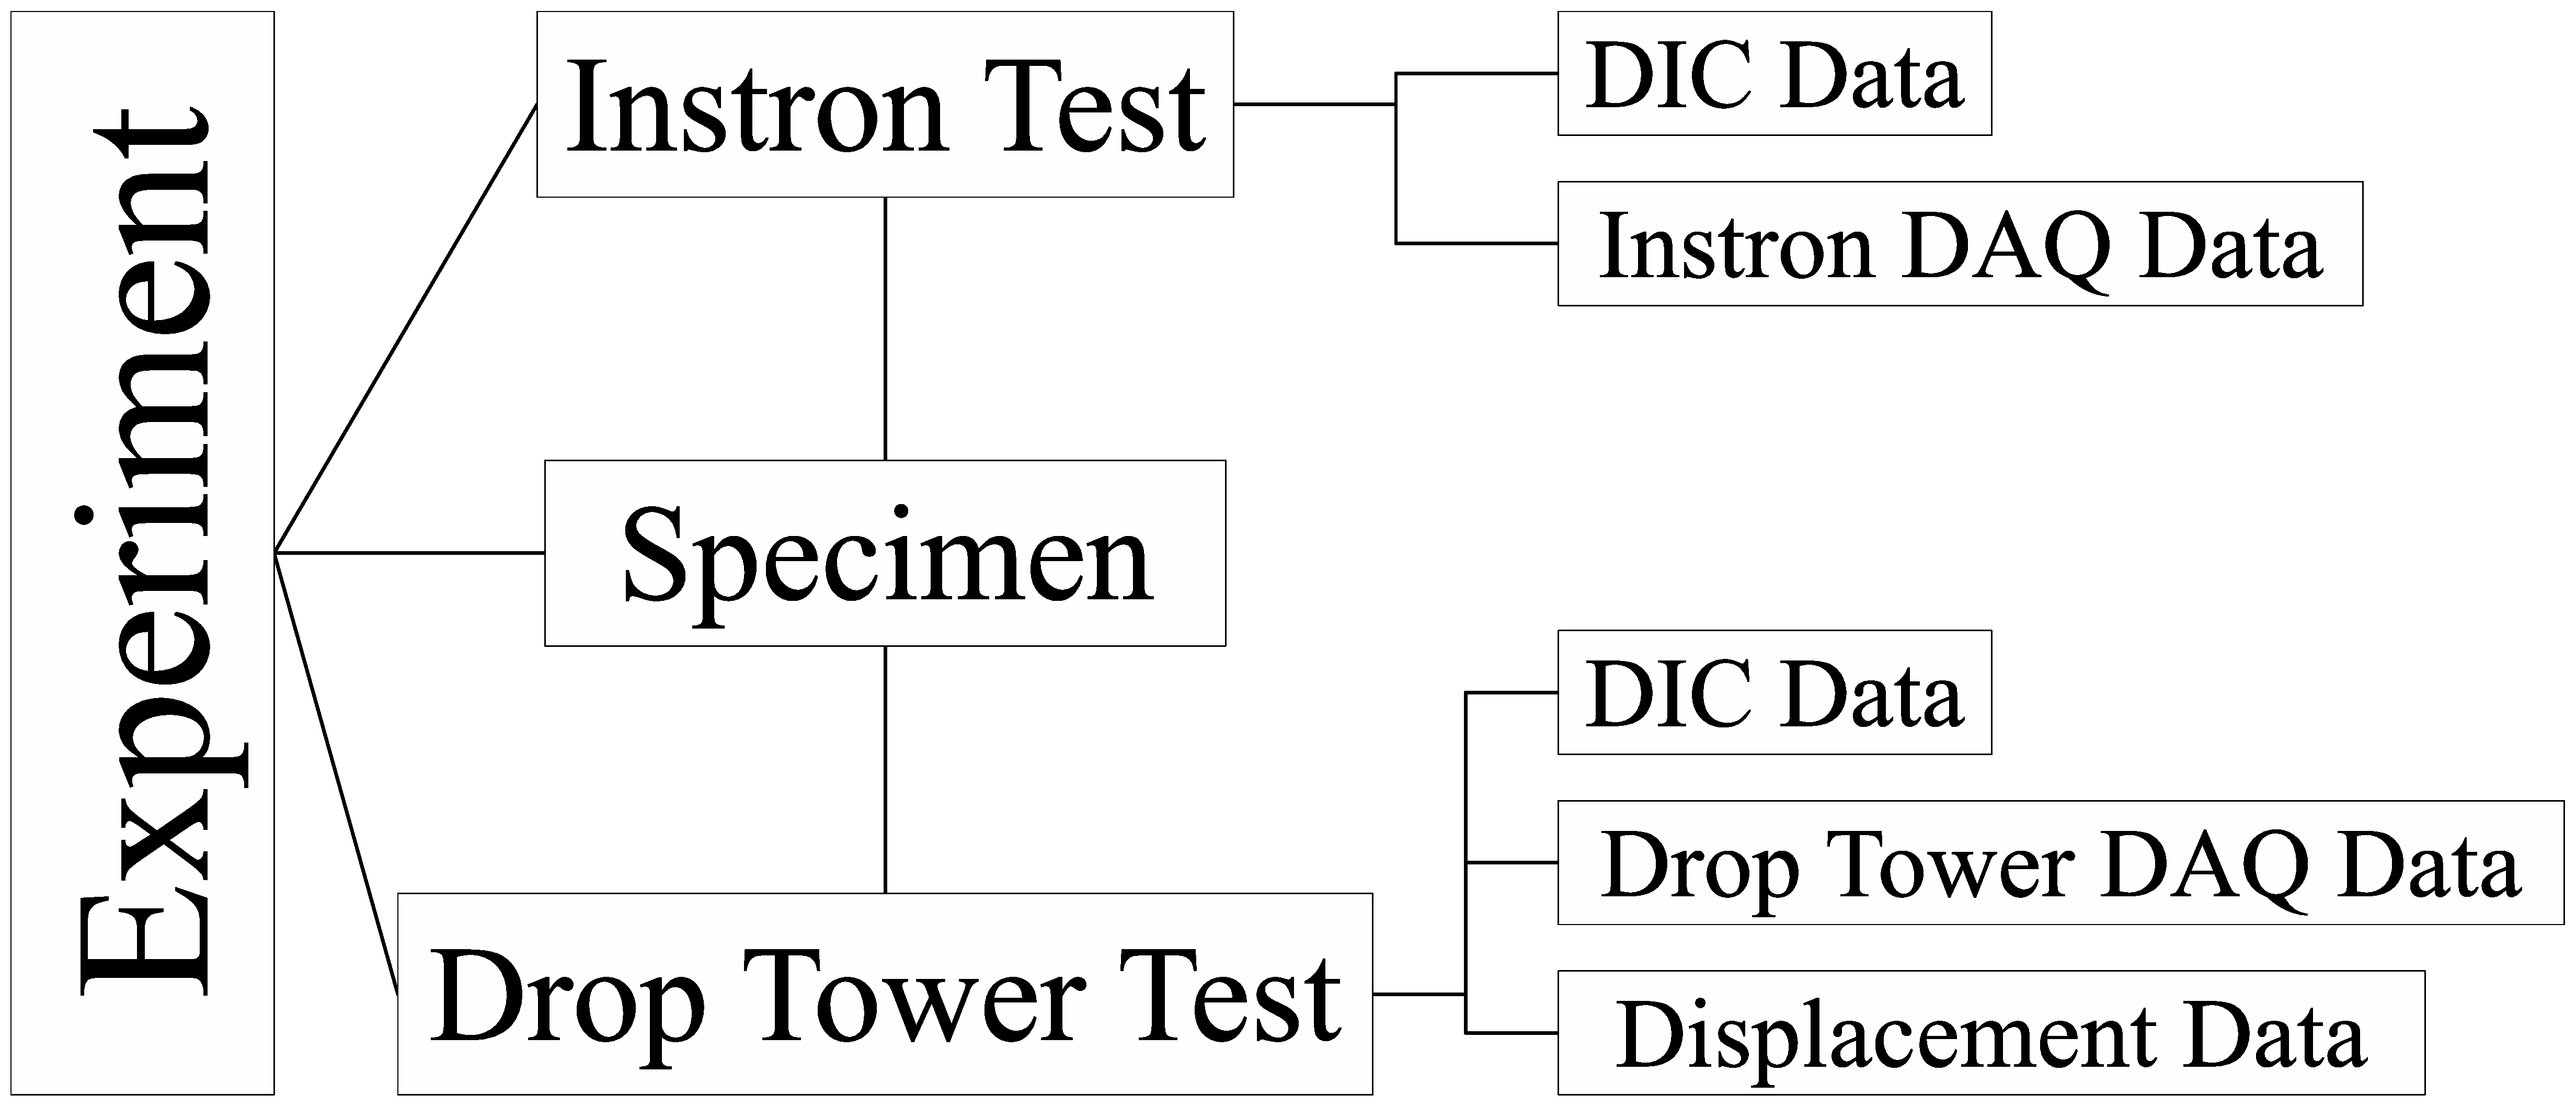
\includegraphics[width=\linewidth]{./appendixCode/analysisCode/Figures/AnalysisHigherarchy}
\caption[Data analysis hierarchy]{The hierarchy of the experimental data analysis. Each box is a Matlab class. Graphic \textcopyright Seth Gilchrist, 2013.}
\label{fig:AnalysisHigherarchy}
\end{figure}

The reason for implementing the code in this way was so that all details of a given analysis would be preserved, in one location, for later review.
If, for example, one wanted to know the filter order used to prepare the displacement data, this could found using the command 

\texttt{>> experiment.GetDropTower.GetDisplacement.GetFilterOrder()}.

Raw data, as well as analysed data, are also stored in the class.
In the end, saving the class object to disk allows for unified saving of all raw data, analysis routines and analysed data in a single \ac{mat}.
 
The code for each of these data analysis classes are given below.
Documentation is built into the MatLab files, so once they are placed in the current MatLab directory or path, help can be found by typing ``\texttt{help <Class Name>.<Method Name>}" at the command line.
Alternatively, all methods are documented in the code.

\subsection{Example input}
\label{sec:code_dt_ins_analysis_example}
Assuming that the data for the desired analysis are stored in ``C:\textbackslash Data\textbackslash TestData\textbackslash", an analysis can be carried out using the following code.
\begin{singlespace}
\begin{lstlisting}
% Fill in the specimen data
name = 'specimen01';
gender = 'm';
age = 80;
height = 170;
weight = 60;
dxa = struct('neck',0.67,'troch',.70,'inter',.70,'total',.75,'wards',0);
op = 'osteopenia';
data = struct('InstronDAQ',1,'InstronDIC',1,'DropTowerDAQ',1,'DropTowerDisplacement',1,'DropTowerDIC',1);

% create the specimen object
specimen = Specimen(name,gender,age,height,weight,dxa,op,data);

% create the experiment object. All sub-objects (DAQ analyses, etc) will be created based on the data structure.
experiment = Experiment(specimen);

% Get the Instron analysis
instronAnalysis = experiment.GetInstron();

% Setup the Instron DAQ parameters
instronAnalysis.GetDAQData.SetFileName('C:\Data\TestData\InstronDAQ.csv');
instronAnalysis.GetDAQData.ReadFile();

instronAnalysis.GetDAQData.SetSampleRate(20000);
instronAnalysis.GetDAQData.SetFilterCutoff(500);
instronAnalysis.GetDAQData.SetGainDisplacement(.35);
instronAnalysis.GetDAQData.SetGainLoad(1200);

% Setup the Instron DIC
instronAnalysis.GetDICData.SetFileName('C:\Data\TestData\InstronDIC.csv');
instronAnalysis.GetDICData.ReadFile();

instronAnalysis.GetDICData.SetSampleRate(100)
instronAnalysis.GetDICData.SetStartTime(0.85)

% Get the drop tower analysis
dropTowerAnalysis = experiment.GetDropTower();

% Setup the drop tower DAQ
dropTowerDAQ = dropTowerAnalysis.GetDAQData();
dropTowerDAQ.SetFileName('C:\Data\TestData\DropTowerDAQ.csv');
dropTowerDAQ.ReadFile();

dropTowerDAQ.SetExcitation(12);
dropTowerDAQ.SetSampleRate(20000);
dropTowerDAQ.SetFilterCutoff(500);
dropTowerDAQ.SetFilterOrder(4);

% Setup the drop tower displacement
dropTowerDisp = dropTowerAnalysis.GetDisplacementData();
dropTowerDisp.SetFileName('C:\Data\TestData\DropTowerDAQ.csv');
dropTowerDisp.ReadFile();

dropTowerDisp.SetSampleRate(9600);
dropTowerDisp.SetFilterCutoff(500);
dropTowerDisp.SetTimeStart(-0.05);
dropTowerDisp.SetFilterOrder(2);

% Setup the drop tower DIC
dropTowerDIC = dropTowerAnalysis.GetDICData();
dropTowerDIC.SetFileName('C:\Data\TestData\DropTowerDIC.csv');
dropTowerDIC.ReadFile();

dropTowerDIC.SetStartTime(-.03);
dropTowerDIC.SetSampleRate(10000);

% Run the analysis
experiment.update(1);

% Save the resulting data
save('C:\Data\TestData\Specimen01.mat','experiment');
\end{lstlisting}
\end{singlespace}
\begin{singlespace}
\subsection{Specimen class}
\begin{lstlisting}
classdef Specimen < handle
    properties (SetAccess = private,Hidden = true)
        % immutables properties of each specimen
        m_specimenName;
        m_gender;
        m_dxa;
        m_opStatus;
        m_age;
        m_height;
        m_weight;
        m_dataAvailable;
        % these are bools to say if the data is available
    end
    methods
        function SP = Specimen(name,gender,age,height,weight,dxa,op,data)
            % The constructor takes the name, DXA values the osteoporosis
            % status and the available data as inputs.
            % name is a string
            % gender is one of: 'm' or 'f' - use 'u' for unknown
            % age is a number in years - use 0 for unknown
            % height is a number in cm - use 0 for unknown
            % weight is a number in kg - use 0 for unknown
            % dxa is a structure with fields:
            %      'neck','troch','inter','total','wards'
            % op is one of:
            %      'normal','osteopenia','osteoporosis','unknown'
            % data is a structure of bools indicating what data with 
            % is available. It is comprised of the fields:
            %      'InstronDAQ','InstronDIC','DropTowerDAQ','DropTowerDisplacement','DropTowerDIC'
            %
            % Sp = Specimen([SpecimenName],[gender],[age],[height],[weight],[DXAValues],[OPStatus],[Data])
            SP.SetSpecimenName(name);
            SP.SetDXA(dxa);
            SP.SetOpStatus(op);
            SP.SetAge(age);
            SP.SetHeight(height);
            SP.SetWeight(weight);
            SP.SetGender(gender);
            SP.SetDataAvailable(data);
        end
        
        function SetSpecimenName(SP,name)
            % A function to set the specimen name.
            %
            % SP.SetSpecimenName(name)
            %
            if ~ischar(name)
                error('No specimen name given. Aborting.')
            end
            SP.m_specimenName = name;

        end
        
        function SetDXA(SP,dxa)
            % A function to set the specimen DXA structure in g/cm^2.
            % The structure must have fields:
            %   neck
            %   troch
            %   inter
            %   total
            %   wards
            %
            % SP.SetDXA(DXA)
            %
            if (~isfield(dxa,'neck') || ~isfield(dxa,'troch') || ~isfield(dxa,'inter') || ~isfield(dxa,'total') || ~isfield(dxa,'wards') )
                error('Specimen:dxaFault','Malformed DXA structure. Please check the DXA data for %s and retry. Aborting.\n',SP.m_specimenName);
            end
            SP.m_dxa = dxa;
        end
        
        function SetOpStatus(SP,op)
            % A function to set the osteoporosis state of the specimen.
            % The value must be one of:
            %   normal
            %   osteopenia
            %   osteoporosis
            %
            % SP.SetOpStatus(status)
            %
            if (~strcmp(op,'normal') && ~strcmp(op,'osteopenia') && ~strcmp(op,'osteoporosis') &&~strcmp(op,'unknown' ))
                error('Specimen:opFault','Invalid osteoporosis state specified. Please check the value for %s and retry. Aborting.\n',SP.m_specimenName);
            end
            SP.m_opStatus = op;
        end
        
        function SetAge(SP,age)
            % A function to set the age of the specimen donor in years.
            % The value must be numeric. Use 0 for unknown.
            %
            % SP.SetAge(age)
            %
            if (~isnumeric(age))
                error('Specimen:ageFault','A non-numeric age was specified for %s.\n',SP.m_specimenName);
            end
            SP.m_age = age;
        end
        
        function SetHeight(SP,height)
            % A function to set the height of the specimen donor in cm.
            % The value must be numeric. Use 0 for unknown.
            %
            % SP.SetHeight(height)
            %
            if (~isnumeric(height))
                error('Specimen:heightFault','A non-numeric height was specified for %s.\n',SP.m_specimenName);
            end
            SP.m_height = height;
        end
        
        function SetWeight(SP,weight)
            % A function to set the weight of the specimen donor in kg.
            % The value must be numeric. Use 0 for unknown.
            %
            % SP.SetWeight(weight)
            %
            if(~isnumeric(weight))
                error('Specimen:weightFault','A non-numeric weight was specified for %s.\n',SP.m_specimenName);
            end
            SP.m_weight = weight;
        end
        
        function SetGender(SP,gender)
            % A function to set the gender of the specimen donor. The
            % value must be one of:
            %   m
            %   f
            %
            % SP.SetGender(gender)
            %
            if (~strcmp(gender,'m') && ~strcmp(gender,'f') && ~strcmp(gender,'u'))
                error('Specimen:genderFault','An invalid gender was supplied for %s.\n',SP.m_specimenName);
            end
            SP.m_gender = gender;
        end
        
        function SetDataAvailable(SP,data)
            % A function to set the data available structure for the
            % specimen. The structure uses bools to indicated if a certain
            % type of data is available for analysis. The structure
            % must have fields:
            %   InstronDAQ
            %   InstronDIC
            %   DropTowerDAQ
            %   DropTowerDisplacement
            %   DropTowerDIC
            %
            % SP.SetDataAvailable(data)
            %
            if ( ~isfield(data,'InstronDAQ') || ~isfield(data,'InstronDIC') || ~isfield(data,'DropTowerDAQ') || ~isfield(data,'DropTowerDisplacement') || ~isfield(data,'DropTowerDIC') )
                error('Specimen:dataFault','Malformed data available structure. Please check the values for %s and retry.\n',SP.m_specimenName);
            end
            SP.m_dataAvailable  = data;
        end
        
        % get functions for each property
        function o = GetSpecimenName(SP)
            % A function to get the specimen name.
            %
            % Name = SP.GetSpecimenName()
            %
            o = SP.m_specimenName;
        end
        function o = GetDXA(SP)
            % A function to get the specimen DXA in g/cm^2. The structure
            % will have fields:
            %   neck
            %   troch
            %   inter
            %   total
            %   wards
            %
            % DXA = SP.GetDXA()
            %
            o = SP.m_dxa;
        end
        function o = GetOpStatus(SP)
            % A function to get the specimen osteoporosis state.
            %
            % OPStatus = SP.GetOpStatus()
            %
            o = SP.m_opStatus;
        end
        function o = GetAge(SP)
            % A function to get the specimen donor age in years.
            %
            % Age = SP.GetAge()
            %
            o = SP.m_age;
        end
        function o = GetHeight(SP)
            % A function to get the height of the specimen donor in cm.
            %
            % Height = SP.GetHeight()
            %
            o = SP.m_height;
        end
        function o = GetWeight(SP)
            % A function to get the weight of the specimen donor in kg.
            %
            % Weight = SP.GetWeight()
            %
            o = SP.m_weight;
        end
        function o = GetGender(SP)
            % A function to get the gender of the specimen donor. The
            % value will be one of:
            %   m
            %   f
            %
            % Gender = SP.GetGender()
            %
            o = SP.m_gender;
        end
        function o = GetDataAvailable(SP)
            % A function to get the data available structure. The structure
            % uses bools to indicate the availability of certain data
            % sources. The structure will have fields:
            %   InstronDAQ
            %   InstronDIC
            %   DropTowerDAQ
            %   DropTowerDisplacement
            %   DropTowerDIC
            %
            % Data = SP.GetDataAvailable()
            %
            o = SP.m_dataAvailable;
        end

        
        function PrintSelf(SP)
            % A function to print the state of the specimen object.
            %
            % SP.PrintSelf()
            %
            fprintf(1,'\n%%%%%%%%%% Specimen Class Data %%%%%%%%%%\n');
            fprintf(1,'Specimen name: %s\n',SP.GetSpecimenName());
            fprintf(1,'Specimen dnoor gender: %s\n',SP.GetGender());
            fprintf(1,'Specimen donor age: %d years\n',SP.GetAge());
            fprintf(1,'Specimen donor height: %d cm\n',SP.GetHeight());
            fprintf(1,'Specimen donor weight: %0.4f kg\n',SP.GetWeight());
            dxaData = SP.GetDXA();
            fprintf(1,'Specimen DXA values (g/cm^2):\n\tNeck:  %f\n\tTroch: %f\n\tInter: %f\n\tTotal: %f\n\tWards: %f\n',dxaData.neck,dxaData.troch,dxaData.inter,dxaData.total,dxaData.wards);
            fprintf(1,'Specimen osteoporosis state: %s\n',SP.GetOpStatus());
            dataAva = SP.GetDataAvailable();
            fprintf(1,'Specimen data fields available:\n\tInstronDAQ:            %d\n\tInstronDIC:            %d\n\tDropTowerDAQ:          %d\n\tDropTowerDisplacement: %d\n\tDropTowerDIC:          %d\n',dataAva.InstronDAQ,dataAva.InstronDIC,dataAva.DropTowerDAQ,dataAva.DropTowerDisplacement,dataAva.DropTowerDIC);
        end
        
    end
end
\end{lstlisting}


\subsection{Experiment class}
\begin{lstlisting}
classdef Experiment < handle
    properties (SetAccess = private, Hidden = false)
        % objects for data sets
        m_specimen;
        m_dropTower;
        m_instron;
    end
    properties (SetAccess = private, Hidden = true)
        % analysis properties
        m_stiffnessDelta;
        m_energyToForceInstronMaxDelta;
        m_strainAtForceInstronMaxDelta;
    end % properties
    
    methods
        function EXP = Experiment(specimen)
            % A constructor for an experiment. Takes a specimen as the
            % input. See Specimen.m for details on creating a specimen.
            %
            % EXP = Experiment(specimen)
            %
            EXP.m_specimen = specimen;
            if (specimen.GetDataAvailable().InstronDAQ || specimen.GetDataAvailable().InstronDIC )
                EXP.m_instron = InstronAnalysis(specimen);
            end
            if (specimen.GetDataAvailable().DropTowerDAQ || specimen.GetDataAvailable().DropTowerDisplacement || specimen.GetDataAvailable().DropTowerDIC)
                EXP.m_dropTower = DropTowerAnalysis(specimen);
            end
        end
        
        function o = GetSpecimen(EXP)
            % A function to get the specimen object used to create the
            % Experiment object
            %
            % Specimen = EXP.GetSpecimen()
            %
            o = EXP.m_specimen;
        end
        
        function o = GetDropTower(EXP)
            % A function to get the drop tower analysis object.
            %
            % DropTowerAnalysis = EXP.GetDropTower()
            %
            o = EXP.m_dropTower;
        end
        
        function o = GetInstron(EXP)
            % A function to get the instron analysis object.
            %
            % InstronAnalysis = EXP.GetInstron()
            %
            o = EXP.m_instron;
        end
        
        function o = GetStiffnessDelta(EXP)
            % A function to get the difference in stiffness between the
            % instron and drop tower in N/m, calculated as:
            %    InstronStiffness - DropTowerStiffness
            %
            % Difference = EXP.GetStiffnessDelta()
            %
            o = EXP.m_stiffnessDelta;
        end
        
        function o = GetEnergyToForceInstronMaxDelta(EXP)
            % A function to get the difference in energy in J between the
            % instron and drop tower, calculated as:
            %    InstronEnergy - DropTowerEnergy
            %
            % Difference = EXP.GetEnergyToForceInstronMaxDelta()
            %
            o = EXP.m_energyToForceInstronMaxDelta;
        end
        
        function o = GetStrainAtForceInstronMaxDelta(EXP)
            % A function to get the difference in strain at the 
            % max instron force in absolute strain. Uses the strain gauge
            % on the instron side, and DIC on the drop tower.
            % The calculation is:
            %    InstronStrain - DropTowerStrain
            %
            % Difference = EXP.GetStrainAtForceInstronMaxDelta()
            %
            o = EXP.m_strainAtForceInstronMaxDelta;
        end        
        
        function Update(EXP,recalcMax)
            % A function to update the state of the analysis.
            %
            % The optional input "recalcMax" is a bool flag to indicate if
            % the drop tower max force should be recalculated. The default
            % value is 1 (yes, recalculate)
            %
            % EXP.Update(recalcMax)
            %
            if nargin<1
                recalcMax = 1;
            end
            ins = EXP.GetInstron();
            dt = EXP.GetDropTower();
            
            % update the child objects
            if ~isempty(ins)
                ins.Update();
                insExist = 1;
                % if the drop tower analysis is present, set the instron max force
                if ~isempty(dt)
                    dt.SetForceInstronMax(ins.GetForceMax())
                end
            else
                insExist = 0;
            end
            if ~isempty(dt)
                dt.Update(recalcMax);
                dtExist = 1;
            else
                dtExist = 0;
            end
            
            
            % if both stiffnesses are available, calculate the stiffness difference
            if ( dtExist && insExist )
                if ( ~isempty(dt.GetStiffness()) && ~isempty(ins.GetStiffness()) )
                    EXP.CalcStiffnessDelta();
                end
            end
            
            % if both energies to max instron are available, calc difference
            if ( dtExist && insExist )
                if ( ~isempty(dt.GetEnergyToForceInstronMax()) && ~isempty(ins.GetEnergy()) )
                    EXP.CalcEnergyDelta();
                end
            end
            
            % if both strains to max instron ara available, calc difference
            if (dtExist && insExist )
                if ( ~isempty(dt.GetStrainDICAtForceInstronMax()) && ~isempty(ins.GetStrainAtMaxGauge()) )
                    EXP.CalcStrainAtForceInstronMaxDelta();
                end
            end
        end
        
        function PrintSelf(EXP)
            % A function to print the current state of the experimental
            % analysis.
            %
            % EXP.PrintSelf()
            %
            
            fprintf(1,'\n%%%%%%%%%% Experiment Class Data %%%%%%%%%%\n');
            EXP.GetSpecimen().PrintSelf();
            fprintf(1,'\n %%%% Scalar Members %%%%\n');
            fprintf(1,'Instron - Drop tower stiffness: %f N/m\n',EXP.GetStiffnessDelta());
            fprintf(1,'Instron - Drop tower energy: %f J\n',EXP.GetEnergyToForceInstronMaxDelta());
            fprintf(1,'Instron - Drop tower strain: %f strain\n',EXP.GetStrainAtForceInstronMaxDelta());
            
            if ~isempty(EXP.GetInstron())
                EXP.GetInstron.PrintSelf();
            else
                fprintf(1,'No InstronAnalysis object associated');
            end
            if ~ isempty(EXP.GetDropTower())
                EXP.GetDropTower().PrintSelf();
            else
                fprintf(1,'No DropTowerAnalysis object associated');
            end
        end
    end % public methods
    
    methods (Access = private, Hidden = true)
        function CalcStiffnessDelta(EXP)
            % A function to calculate the difference in stiffness between
            % the instron and drop tower tests. The calculation is:
            %   InstronStiffness - DropTowerStiffness
            %
            % EXP.CalcStiffnessDelta()
            %
            stiffnessInstron = EXP.GetInstron().GetStiffness();
            stiffnessDropTower = EXP.GetDropTower().GetStiffness();
            
            EXP.m_stiffnessDelta = stiffnessInstron - stiffnessDropTower;
        end
        
        function CalcEnergyDelta(EXP)
            % A function to calculate the differenc in energy between the
            % instron and drop tower tests. The calculation is:
            %    InstronEnergy - DropTowerEnergy
            %
            % EXP.CalcEnergyDelta()
            %
            energyInstron = EXP.GetInstron().GetEnergy();
            energyDropTower = EXP.GetDropTower().GetEnergyToForceInstronMax();
            
            EXP.m_energyToForceInstronMaxDelta = energyInstron - energyDropTower;
        end
        
        function CalcStrainAtForceInstronMaxDelta(EXP)
            % A function to calculate the difference in strain at the 
            % max instron force in absolute strain. Uses the strain gauge
            % on the instron side, and DIC on the drop tower.
            % The calculation is:
            %    InstronStrain - DropTowerStrain
            %
            % EXP.CalcStrainAtForceInstronMaxDelta()
            %
            strainInstron = EXP.GetInstron().GetStrainAtMaxGauge();
            strainDropTower = EXP.GetDropTower().GetStrainDICAtForceInstronMax();
            
            EXP.m_strainAtForceInstronMaxDelta = strainInstron - strainDropTower;
        end
    end % private methods
end
\end{lstlisting}


\subsection{Instron test class}
\begin{lstlisting}
classdef InstronAnalysis < handle
    properties (SetAccess = private, Hidden = false)
        % members from the specimen
        m_specimen;
        % members from the DAQ equipment
        m_daqData;
        % members from the dic
        m_dicData;          % only used if DIC data is available.
    end
    
    properties( SetAccess = private, Hidden = true)    
        % machine members
        m_instronCompliance = 1/30118000; % m/N loading plate compliance
        m_commonTimeRate = 5000; % Hz
        
        % result vectors members from interpolation analysis
        m_time;             % in seconds
        m_force;            % in newtons, compressive force
        m_displacementTroch;    % in m compression
        m_displacementPlaten;   % in m compression
        m_compression;      % in m. Specimen compression
        m_strainGauge; % [Gauge1, Gauge2, Gauge3]
        m_strainPrincipalGauge; %[P1, P2, Angle]
        m_strainDIC;
        m_strainError;
        
        % results members from analysis
        m_stiffness;        % in kN/mm
        m_energyToForceMax; % J
        m_strainAtMaxDIC;
        m_strainAtMaxGauge; % in strain, minimum principal stain
        m_frameAtMax;       % the dic frame at max force
        m_forceMax;
        m_timeForceMax;
        m_indexForceMax;
        m_strainErrorMean;
        m_strainErrorStdev;
    end % properties
    
    methods
        function IA = InstronAnalysis(specimen)
            % The constructor for the InstronAnalysis class. See
            % Specimen.m for details.
            %
            % IA = InstronAnalysis(specimen)
            %
            IA.m_specimen = specimen;
            if IA.GetSpecimen().GetDataAvailable().InstronDAQ
                IA.m_daqData = DAQInstron(specimen);
            end
            if IA.GetSpecimen().GetDataAvailable().InstronDIC
                IA.m_dicData = DICData(specimen);
            end
        end

        function o = GetSpecimen(IA)
            % A function to get the specimen object
            %
            % Specimen = IA.GetSpecimen()
            %
            o = IA.m_specimen;
        end

        function o = GetDICData(IA)
            % A function to get the DIC data object.
            %
            % DICData = IA.GetDICData()
            %
            o = IA.m_dicData;
        end

        function o = GetDAQData(IA)
            % A function to get the DAQ data object.
            %
            % DAQData = IA.GetDAQData()
            %           
            o = IA.m_daqData;
        end
    
        function SetInstronCompliance(IA,compliance)
            % A function to set the compliance of th testing rig in m/N.
            % The default value is 1/30118000 m/N.
            %
            % Compliance = IA.SetInstronCompliance(compliance)
            %
            IA.m_instronCompliance = compliance;
        end
        
        function o = GetInstronCompliance(IA)
            % A function to get the compliance of the instron in m/N.
            %
            % Compliance = GetInstronCompliance()
            %
            o = IA.m_instronCompliance;
        end

        function o = GetCommonTimeRate(IA)
            % A function to get the common time rate in Hz.
            %
            % Rate = IA.GetCommonTimeRate()
            %
            o = IA.m_commonTimeRate;
        end
        
        function SetCommonTimeRate(IA,rate)
            % A function to set the common time rate in Hz. The default
            % is 5 kHz.
            %
            % IA.SetCommonTimeRate(rate)
            %
            if IA.m_commonTimeRate ~= rate
                IA.m_commonTimeRate = rate;
            end
        end
        
        function InterpolateDICToCommonTime(IA)
            % A function to interpolate the data from the DIC object to the
            % common time vector.
            %
            % IA.InterpolateDICToCommonTime()
            %
            IA.m_strainDIC = interp1(IA.GetDICData.GetTime(), IA.GetDICData().GetStrainData(), IA.GetTime());
        end

        function o = GetTime(IA)
            % A function to get the time vector in seconds.
            %
            % Time = IA.GetTime()
            %
            if isempty(IA.m_time)
                IA.CreateCommonTimeVector();
            end
            o = IA.m_time;
        end
        
        function o = GetForce(IA)
            % A function to get the force in the instron analysis time
            % frame in newtons.
            %
            % Force = IA.GetForce()
            %
            o = IA.m_force;
        end
        
        function o = GetPrincipalStrainGauge(IA)
            % A function to get the first principal strain from the gauge
            % in the instron analysis time frame in absolute strain.
            % Outputs strain as
            %   [principal1,principal2,angle] 
            % with the strains in absolute and the angle in radians
            %
            % PrincipalStrain = IA.GetPrincipalStrainGauge();
            %
            o = IA.m_strainPrincipalGauge;
        end
        
        function o = GetStrainGauge(IA)
            % A function to get the stain gauge data in the instron 
            % anslysis time frame. Output as [gauge1,gauge2,gaue3] in
            % absolute strain.
            %
            % Strain = IA.GetStrainGauge()
            %
            o = IA.m_strainGauge;
        end
        
        function o = GetStrainDIC(IA)
            % A function to get the DIC strain in the instron analysis time
            % frame in absolute strain.
            %
            % Strain = IA.GetStrainDIC()
            %
            o = IA.m_strainDIC;
        end
        
        function o = GetDisplacementTroch(IA)
            % A function to get the trochanter displacement in mm in the
            % instron analysis time frame.
            %
            % Displacement = IA.GetDisplacementTroch()
            %
            o = IA.m_displacementTroch;
        end
        
        function o = GetDisplacementPlaten(IA)
            % A function to get the platen displacement in mm in the
            % instron analysis time frame.
            %
            % Displacement = IA.GetDisplacementPlaten()
            %            
            o = IA.m_displacementPlaten;
        end
        
        function o = GetCompression(IA)
            % A function to get the specimen compression in mm in the
            % instron analysis time frame.
            %
            % Compression = IA.GetCompression()
            %
            o = IA.m_compression;
        end

        function o = GetForceMax(IA)
            % A function to get the max force in newtons.
            %
            % Force = IA.GetForceMax()
            %
            o = IA.m_forceMax;
        end

        function o = GetTimeForceMax(IA)
            % A function to get the time of the max force in seconds.
            %
            % Time = IA.GetTimeForceMax()
            %
            o = IA.m_timeForceMax;
        end

        function o = GetIndexForceMax(IA)
            % A function to get the index of the max force.
            %
            % Index = IA.GetIndexForceMax()
            %
            o = IA.m_indexForceMax;
        end

        function o = GetIndexAtTime(IA,time)
            % A function to get the index at a give time in seconds.
            % Rounds the index down.
            %
            % Index = IA.GetIndexAtTime(time)
            %
            o = find(IA.GetTime() < time,1,'last');
        end

        function o = GetStiffness(IA)
            % A function to get the stiffness of the specimen in N/m.
            %
            % Stiffness = IA.GetStiffness()
            %
            if isempty(IA.m_stiffness)
                IA.CalcStiffness();
            end
            o = IA.m_stiffness;
        end

        function o = GetEnergy(IA)
            % A function to get the energy during loading in J
            %
            % Energy = IA.GetEnergy(IA)
            %
            if isempty(IA.m_energyToForceMax())
                IA.CalcEnergy();
            end
            o = IA.m_energyToForceMax;
        end
        
        function o = GetStrainAtMaxGauge(IA)
            % A function to calc the minimum principal strain at the strain
            % gauge location at the max force. Returns a value that has
            % been median filtered using a radius of 2.
            %
            % Strain = GetStrainAtMaxGauge()
            %
            if isempty(IA.m_strainAtMaxGauge)
                IA.CalcStrainAtMaxGauge();
            end
            o = IA.m_strainAtMaxGauge;
        end
        
        function o = GetStrainAtMaxDIC(IA)
            % A function to calc the minimum principal strain at the strain
            % gauge location at the max force. Returns a value that has
            % been median filtered using a radius of 2.
            %
            % Strain = GetStrainAtMaxGauge()
            %
            if isempty(IA.m_strainAtMaxDIC)
                IA.CalcStrainAtMaxDIC()
            end
            o = IA.m_strainAtMaxDIC;
        end

        function o = GetFrameAtMax(IA)
            % A function to get the DIC frame at the max force
            %
            % Frame = IA.GetFrameAtMax()
            %
            if isempty(IA.m_frameAtMax)
                IA.CalcFrameAtMax();
            end
            o = IA.m_frameAtMax;
        end

        function o = GetStrainError(IA)
            % A function to get the strain error vector in absolute strain.
            %
            % StrainError = IA.GetStrainError()
            %
            if isempty(IA.m_strainError)
                IA.CalcStrainError()
            end
            o =IA.m_strainError;
        end

        function o = GetStrainErrorMean(IA)
            % A function to get the mean strain error in absolute strain.
            %
            % MeanError = IA.GetStrainErrorMean()
            %
            if isempty(IA.m_strainErrorMean)
                IA.CalcStrainErrorMean();
            end
            o = IA.m_strainErrorMean;
        end

        function o = GetStrainErrorStdev(IA)
            % A function to get the strain error standard deviation in
            % absolute strain.
            %
            % StrainStdev = IA.GetStrainErrorStdev()
            %
            if isempty(IA.m_strainErrorStdev)
                IA.CalcStrainErrorStdev();
            end
            o = IA.m_strainErrorStdev;
        end
        


        function o = GetCompressionAtTime(IA,time)
            % A function to get the specimen compression in mm at a given time 
            % in seconds. Output is linearly interpolated from the compression
            % vector.
            %
            % Compression = GetCompressionAtTime(time)
            %
            o = interp1(IA.GetTime(),IA.GetCompression(),time);
        end
        
        function o = GetForceAtTime(IA,time)
            % A function to get the force in newtons at a give time in
            % seconds. The output is linearly interpolated from the time
            % vecvtor.
            %
            % Force = IA.GetForceAtTime(time)
            %
            o = interp1(IA.GetTime(),IA.GetForce(),time);
        end
                
        function Update(IA)
            % A function to update the state of the Instron analysis. Does
            % not execute ReadFile() which must be done by the user.
            %
            % IA.Update()
            %
            
            % Check if DAQ analysis will be done
            if ~isempty(IA.GetDAQData())
                % if there is a DAQ data object. Call its update function
                IA.GetDAQData.Update();
                   
                % next put everything into the common time vector for the
                % analysis. If there is DIC data it will also be
                % interpolated into this time space
                IA.InterpolateDAQToCommonTime()
                
                % Find the max force and its time and index
                IA.CalcForceMax()
                % Find the stiffness
                IA.CalcStiffness()
                % Find the energy to max force
                IA.CalcEnergy()
                % Find the gauge strain at max force
                IA.CalcStrainAtMaxGauge()
            end
            
            if ~isempty(IA.GetDICData()) % check for DIC data
                errorFlag = 0;
                if ~ischar(IA.GetDICData.GetFileName)
                   warning('InstronAnalysis:FileNameDIC','This error is fatal. No DIC file name for specimen %s was provided before calling AnalyzeInstronData.\n',IA.GetSpecimen().GetSpecimenName());
                   errorFlag = errorFlag + 1;
                end
                if isempty(IA.GetDICData.GetTimeStart)
                    warning('InstronAnalysis:StartTimeDIC','This error is fatal. No DIC start time has been set for specimen %s. Without the start time the DIC data cannot be matched to the DAQ data.\n',IA.GetSpecimen().GetSpecimenName());
                    errorFlag = errorFlag + 1;
                end
                if isempty(IA.GetDICData.GetSampleRate)
                    warning('InstronAnalysis:SampleRateDIC','This error is fatal. No DIC sample rate has been set for specimen %s. Without this sample rate the DIC frame corresponding to max force cannot be found.\n',IA.GetSpecimen().GetSpecimenName());
                    errorFlag = errorFlag + 1;
                end
                if errorFlag
                    error('InstronAnalysis:AnalyzeDICData','%d errors were detected when preparing to analyzde the Instron DIC data for specimen %s.\n',errorFlag,IA.GetSpecimen().GetSpecimenName());
                end
                               
                % next interpolate the data to the common time vector
                IA.InterpolateDICToCommonTime()
            end
            
            if ~isempty(IA.GetDICData()) && ~ isempty(IA.GetDAQData()) % things that require both for calculation
                % calculate the error
                IA.CalcStrainError()
                % calculate the mean error
                IA.CalcStrainErrorMean()
                % calculate the error standard deviation
                IA.CalcStrainErrorStdev()
                % determine the frame at which the max force occured
                IA.CalcFrameAtMax()
                % calculate the strain from the DIC at the max force using
                % a median filter radius of 2 (the default)
                IA.CalcStrainAtMaxDIC(2)
            end
        end

        function PrintSelf(IA)
            % A function to print the current state of the Instron analysis
            % object
            %
            % IA.PrintSelf()
            %
            fprintf(1,'\n%%%%%%%%%% Instron Analysis Class Data %%%%%%%%%%\n');
            IA.GetSpecimen().PrintSelf();
            
            fprintf(1,'\n  %%%% Instron Analysis Class Parameters %%%%\n');
            fprintf(1,'Instron compliance: %e m/N\n',IA.GetInstronCompliance());
            fprintf(1,'Specimen stiffness: %f N/m\n',IA.GetStiffness());
            fprintf(1,'Maximum force: %f N\n',IA.GetForceMax());                  
            fprintf(1,'Time at max force: %f seconds\n',IA.GetTimeForceMax());
            fprintf(1,'Index at max force: %d\n',IA.GetIndexForceMax());
            fprintf(1,'Energy to max force: %f J\n',IA.GetEnergy());
            fprintf(1,'DIC min principal strain at max force: %f strain\n',IA.GetStrainAtMaxDIC());
            fprintf(1,'Gauge min principal strain at max force: %f strain\n',IA.GetStrainAtMaxGauge());
            fprintf(1,'DIC frame at max force: %d\n',IA.GetFrameAtMax());
            fprintf(1,'DIC min principal strain mean error: %f strain\n',IA.GetStrainErrorMean());
            fprintf(1,'DIC min principal strain error stdev: %f strain\n',IA.GetStrainErrorStdev());
            
            fprintf(1,'\n  %%%% Instron Analysis Data %%%%\n');
            fprintf(1,'Instron time: [%d,%d] in seconds\n',size(IA.GetTime()));
            fprintf(1,'Instron force: [%d,%d] in newtons\n',size(IA.GetForce()));
            fprintf(1,'Instron trochanter displacement: [%d,%d] in m\n',size(IA.GetDisplacementTroch()));
            fprintf(1,'Instron platen displacement: [%d,%d] in m\n',size(IA.GetDisplacementPlaten()));
            fprintf(1,'Instron specimen compression: [%d,%d] in m\n',size(IA.GetCompression()));
            fprintf(1,'Instron strain gauge: [%d,%d] in strain\n',size(IA.GetStrainGauge()));
            fprintf(1,'Instron gauge principal strain: [%d,%d] in strain and radians\n',size(IA.GetPrincipalStrainGauge()));
            fprintf(1,'Instron DIC principal strain: [%d,%d] in strain\n',size(IA.GetStrainDIC()));
            fprintf(1,'Instron DIC-Guage strain error: [%d,%d] in strain\n',size(IA.GetStrainError()));
            
            if ~isempty(IA.GetDAQData())
                IA.GetDAQData().PrintSelf();
            else
                fprintf(1,'\n%%%%%%%%%% No DAQ Data Available %%%%%%%%%%\n');
            end
            if ~isempty(IA.GetDICData())
                IA.GetDICData().PrintSelf();
            else
                fprintf(1,'\n%%%%%%%%%% No DIC Data Available %%%%%%%%%%\n');
            end
        end
    end % public methods
    methods (Access = private,Hidden = true)
        function CreateCommonTimeVector(IA)
            % A function to create the common time vector to use in the
            % instron analysis in seconds.
            %
            % IA.CreateCommonTimeVector()
            %
            time = IA.GetDAQData.GetTime;
            IA.m_time = 0.2:1/IA.GetCommonTimeRate():max(time);
        end

        function InterpolateDAQToCommonTime(IA)
            % A function to interpolate the data from the DAQ data object
            % into the common time vector
            %
            % IA.InterpolateDAQToCommonTime()
            %
            IA.m_force = -interp1(IA.GetDAQData.GetTime(), IA.GetDAQData.GetForce(), IA.GetTime() ); % negative to get compressive force
            
            IA.m_displacementTroch = -interp1(IA.GetDAQData.GetTime(), IA.GetDAQData.GetDisplacement(), IA.GetTime());
            IA.m_displacementPlaten = IA.GetForce().* IA.GetInstronCompliance();
            IA.m_compression = IA.GetDisplacementTroch() - IA.GetDisplacementPlaten;
                     
            IA.m_strainGauge(:,1) = interp1(IA.GetDAQData.GetTime(), IA.GetDAQData.GetStrainGauge1(), IA.GetTime());
            IA.m_strainGauge(:,2) = interp1(IA.GetDAQData.GetTime(), IA.GetDAQData.GetStrainGauge2(), IA.GetTime());
            IA.m_strainGauge(:,3) = interp1(IA.GetDAQData.GetTime(), IA.GetDAQData.GetStrainGauge3(), IA.GetTime());
            
            IA.m_strainPrincipalGauge(:,1) = interp1(IA.GetDAQData.GetTime(), IA.GetDAQData.GetPrincipalStrain1(), IA.GetTime());
            IA.m_strainPrincipalGauge(:,2) = interp1(IA.GetDAQData.GetTime(), IA.GetDAQData.GetPrincipalStrain2(), IA.GetTime());
            IA.m_strainPrincipalGauge(:,3) = interp1(IA.GetDAQData.GetTime(), IA.GetDAQData.GetPrincipalStrainAngle(), IA.GetTime());
        end

        function CalcForceMax(IA)
            % A funtion to find the max force in netons.
            %
            % IA.CalcForceMax()
            %
            [maxF,maxFI] = max(IA.GetForce());
            IA.m_forceMax = maxF;
            time = IA.GetTime();
            IA.m_timeForceMax = time(maxFI);
            IA.m_indexForceMax = maxFI;
        end

        function CalcStiffness(IA)
            % A function to calculate the stiffness of the specimen. Uses
            % the 25% and 75% of the max force to calcualte the
            % stiffness.
            %
            % IA.CalcStiffness()
            %
            if isempty(IA.GetForceMax())
                IA.CalcForceMax()
                warning('InstronAnalysis:ExecutionOrder','Stiffness requested for %s before calculation of max force.\nMax force calculation being executed now.\n',IA.GetSpecimen().GetSpecimenName())
            end 
            % get the second force level for stiffness calculation
            forceOne = IA.GetForceMax()*.75;
            forceTwo = IA.GetForceMax()*.25;
            % get the index for the force at half max force
            indexForceOne = find(IA.GetForce() > forceOne,1,'first');
            indexForceTwo = find(IA.GetForce() > forceTwo,1,'first');
            % get the diplacement at max force
            compression = IA.GetCompression();
            % get the displacement at force two
            dispForceOne = compression(indexForceOne);
            dispForceTwo = compression(indexForceTwo);
            % calculate the stiffness between force two and force max
            stiffness = (forceOne - forceTwo)/(dispForceOne - dispForceTwo);
            % convert to N/m
            IA.m_stiffness = stiffness;
        end

        function CalcEnergy(IA)
            % A function to calculate the energy to the max force
            %
            % IA.CalcEnergy()
            %
            if isempty(IA.GetForceMax())
                warning('InstronAnalysis:ExecutionOrder','Energy to max force requested for %s before calculation of max force.\nMax force calculation being executed now.\n',IA.GetSpecimen().GetSpecimenName())
                 IA.CalcForceMax()           
            end
            % Get the data
            compression = IA.GetCompression();
            force = IA.GetForce();
            % find the valid data
            % numerically integrate using the valid indexes up to the max
            % force index using compression in m.
            IA.m_energyToForceMax = trapz(compression(1:IA.GetIndexForceMax()-1),force(1:IA.GetIndexForceMax()-1));
        end

        function CalcStrainAtMaxGauge(IA,radiusMedianFilter)
            % A function to calculate the minimum principal strain from the
            % strain gague at the max force in absulute strain.  Uses a 
            % median filter for  noise reduction with a default radius of
            % 2.
            %
            % IA.CalcStrainAtMaxGauge(radius(optional))
            %
            if nargin < 2
                radiusMedianFilter = 2;
            end
            principal = IA.GetPrincipalStrainGauge();
            
            IA.m_strainAtMaxGauge = median( principal( IA.GetIndexForceMax()-radiusMedianFilter:IA.GetIndexForceMax()+radiusMedianFilter,2 ) );
        end

        function CalcStrainAtMaxDIC(IA,radiusMedianFilter)
            % A function to calc the DIC strain at the max force. Returns
            % the value in absolute strain, median filtered using a default
            % radius of 2. The optional input can change that radius.
            %
            % IA.CalcStrainAtMaxDIC(radius(optional))
            %
            if nargin < 2
                radiusMedianFilter = 2;
            end
            strain = IA.GetStrainDIC();
            IA.m_strainAtMaxDIC = median( strain( IA.GetIndexForceMax()-radiusMedianFilter:IA.GetIndexForceMax()+radiusMedianFilter ) );
        end

        function CalcFrameAtMax(IA)
            % A function to calculate the DIC frame at the max force.
            %
            % IA.CalcFrameAtMax()
            %
            if isempty(IA.GetTimeForceMax())
                error('InstronAnalysis:DataAvailability','DIC frame at max load for %s requested before time at max load has been set.\n',IA.GetSpecimen().GetSpecimenName());
            end
            if isempty(IA.GetDICData())
                error('InstronAnalysis:DataAvailability','DIC frame at max load for %s requested when no DIC data is available.\n',IA.GetSpecimen().GetSpecimenName());
            end
            IA.m_frameAtMax = floor(( IA.GetTimeForceMax() - IA.GetDICData.GetTimeStart )*IA.GetDICData.GetSampleRate);
        end

        function CalcStrainError(IA)
            % A function to calculate the strain error vector, that is
            % (gauge strain) - (DIC strain) in absolute strain
            %
            % IA.CalcStrainError()
            %
            if ( isempty(IA.GetPrincipalStrainGauge) || isempty(IA.GetStrainDIC()) )
                error('InstronAnalysis:DataAvailability','Strain error requested for %s when either gauge minimum principal strain or DIC minimum principal strain are unavailable.\n',IA.GetSpecimen().GetSpecimenName());
            end
            % subtract the strain gauge P2 from StrainDIC for all time
            principal = IA.GetPrincipalStrainGauge();
            IA.m_strainError = principal(:,2) - IA.GetStrainDIC()';
        end

        function CalcStrainErrorMean(IA)
            % A function to calculate the mean strain error in absolute
            % strain.
            %
            % IA.CalcStrainErrorMean()
            %
            if isempty(IA.GetStrainError())
                error('InstronAnalysis:DataAvailability','Mean strain error requested for %s when strain error vector is unavailable.\n',IA.GetSpecimen().GetSpecimenName());
            end
            % find the last index for which DIC strain is defined and
            % subtract 1 second to remove spike at end of data
            strainError = IA.GetStrainError();
            validData = ~isnan(strainError);
            lastIndex = IA.GetIndexAtTime(IA.GetTimeForceMax+1.5);                     
            IA.m_strainErrorMean = mean(strainError(validData(1:lastIndex)));
        end

        function CalcStrainErrorStdev(IA)
            % A function to calculate the strain error standard deviation
            % in absolute strain
            %
            % IA.CalcStrainErrorStdev()
            %
            if isempty(IA.GetStrainError())
                error('InstronAnalysis:DataAvailability','The standard deviation of the strain error requested for %s when strain error vector is unavailable.\n',IA.GetSpecimen().GetSpecimenName());
            end
            % find the last index for which DIC strain is defined and
            % subtract 1 second to remove spike at end of data
            strainError = IA.GetStrainError();
            validData = ~isnan(strainError);
            lastIndex = find(validData == 1,1,'last')-5000;                        
            IA.m_strainErrorStdev = std(strainError(validData(1:lastIndex)));
        end
    
    end % private methods
end % classdef
\end{lstlisting}


\subsection{Instron \acs*{daq} class}
\begin{lstlisting}
classdef DAQInstron < handle
    properties (SetAccess = private, Hidden = false)
        m_specimen;    
    end

    properties (SetAccess = private, Hidden = true)
        m_forceDAQVoltage;
        m_forceDAQ;
        m_displacementDAQVoltage;
        m_displacementDAQ;
        m_strainGauge1DAQ;
        m_strainGauge2DAQ;
        m_strainGauge3DAQ;
        m_triggerDAQ;
        m_timeDAQ;
        m_fileNameDAQ = '';
        
        % members for filtering and analysis
        m_sampleRate = 0;           % Hz
        m_samplePeriod = 0;         % s
        m_filterCutoff = 0;
        m_filterOrder = 4;
        m_gainDisplacement = 0;     % mm/V
        m_gainLoad = 0;             % N/V        
        
        % post filtering data
        m_force;
        m_displacement;
        m_strainGauge1;
        m_strainGauge2;
        m_strainGauge3;
        m_strainGaugeP1;
        m_strainGaugeP2;
        m_strainGaugePhi;
        m_trigger;
        m_time;
    end % properties
    
    methods (Access = public)
        function DI = DAQInstron(specimen)
            % Constructor for the instron DAQ data class. The single input
            % is a Specimen data object. See Specimen.m for details on
            % the specimen data class.
            %
            % DI = DAQInstron(specimen)
            %            
            DI.m_specimen = specimen;
        end
        
        function o = GetSpecimen(DI)
            % A function to get the specimen data object used to construct
            % the DAQ data object.
            %
            % Specimen = DI.GetSpecimen()
            %
            o = DI.m_specimen;
        end
        
        function SetFileName(DI,file)
            % A function to set the name of the DAQ data file.
            %
            % DI.SetFileName(file)
            %
            if ~strcmp(DI.m_fileNameDAQ,file)
                if ~exist(file,'file')
                    error('DAQInstron:DataAvailability','The specified instron DAQ file for %s does not exist.\n',DI.GetSpecimen().GetSpecimenName());
                end
                DI.m_fileNameDAQ = file;
            end
        end

        function o = GetFileName(DI)
            % A function to get the name of the DAQ data file.
            %
            % File = DI.GetFileName()
            %
            o = DI.m_fileNameDAQ;
        end
        
        function SetSampleRate(DI,rate)
            % A function to set the DAQ sample rate in Hz. The sampling
            % period is automatically updated.
            %
            % DI.SetSampleRate(rate)
            %
            if DI.m_sampleRate ~= rate
                DI.m_sampleRate = rate;
                DI.m_samplePeriod = 1/rate;
            end
        end
        function o = GetSampleRate(DI)
            % A function to get the DAQ sample rate in Hz
            %
            % Rate = DI.GetSampleRate()
            %
            o = DI.m_sampleRate;
        end
        function SetSamplePeriod(DI,period)
            % A function to set the DAQ sampling period in seconds. The
            % sampling rate is automatically updated.
            %
            % DI.SetSamplePeriod(period)
            %
            if DI.m_samplePeriod ~= period
                DI.m_samplePeriod = period;
                DI.m_sampleRate = 1/period;
            end
        end
        function o = GetSamplePeriod(DI)
            % A function to get the DAQ sampling period in seconds.
            %
            % Period = DI.GetSamplePeriod()
            %
            o = DI.m_samplePeriod;
        end
        function SetFilterCutoff(DI,cutoff)
            % A function to set the filter cutoff frequency in Hz.
            %
            % DI.SetFilterCutoff(cutoff)
            %
            if DI.m_filterCutoff ~= cutoff
                DI.m_filterCutoff = cutoff;
            end
        end
        function o = GetFilterCutoff(DI)
            % A function to get the filter cutoff frequency in Hz.
            %
            % Cutoff = DI.GetFilterCutoff()
            %
            o = DI.m_filterCutoff;
        end
        function SetFilterOrder(DI,order)
            % A function to set the filter order. The filter order must
            % be even due to the use of the filtfilt algorithm. The value
            % passed to filtfilt will be the specified order/2. Since
            % filtfilt doubles the order of the filter, the resulting
            % order will be the same as specified here. If an odd order
            % is specified, it will be incremented by one.
            %
            % DI.SetFilterOrder(order)
            %
            if DI.m_filterOrder ~= order
                if mod(order,2)
                    warning('InstronDAQ:DataValues','The filter order for %s was set to an odd number. Only even orders are accepted. The order is being increased by one.\n',DI.GetSpecimen().GetSpecimenName());
                    order = order + 1;
                end
                DI.m_filterOrder = order;
            end
        end
        function o = GetFilterOrder(DI)
            % A function to get the filter order.
            %
            % Order = DI.GetFilterOrder()
            %
            o = DI.m_filterOrder;
        end
        function SetGainDisplacement(DI,gain)
            % A function to set the displacement gain in mm/V.
            %
            % DI.SetGainDisplacement(gain)
            %
            if DI.m_gainDisplacement ~= gain
                DI.m_gainDisplacement = gain;
            end
        end
        function o = GetGainDisplacement(DI)
            % A function to get the displacement gain in mm/V.
            %
            % Gain = DI.GetGainDisplacement()
            %
            o = DI.m_gainDisplacement;
        end
        function SetGainLoad(DI,gain)
            % A function to set the load gain in N/V.
            %
            % DI.SetGainLoad(gain)
            %
            if DI.m_gainLoad ~= gain
                DI.m_gainLoad = gain;
            end
        end
        function o = GetGainLoad(DI)
            % A function to get the load gain in N/V.
            %
            % Gain = DI.GetGainLoad()
            %
            o = DI.m_gainLoad;
        end
        
        function ReadFile(DI)
            % A function to read the file specified by DI.SetFileName(file).
            %
            % DI.ReadFile()
            %
            if isempty(DI.m_fileNameDAQ)
                error('InstronDAQ:DataAvailablity','File read was called for %s when no file name was set.\n',DI.GetSpecimen().GetSpecimenName());
            end
            % read the file
            instron = importdata(DI.m_fileNameDAQ,',');
            % if there was a file header, the result would be a strcut. We
            % want only the data.
            if isstruct(instron)
                instron = instron.data;
            end
            % put the raw data into the correct vectors
            DI.m_timeDAQ = instron(:,1);
            DI.m_forceDAQVoltage = instron(:,6);
            DI.m_displacementDAQVoltage = instron(:,5);
            DI.m_triggerDAQ = instron(:,7);
            DI.m_strainGauge1DAQ = instron(:,2);
            DI.m_strainGauge2DAQ = instron(:,3);
            DI.m_strainGauge3DAQ = instron(:,4);
        end

        function o = GetTime(DI)
            % A function to get the time vector in seconds, with t = 0
            % at the time of the trigger.
            %
            % Time = DI.GetTime()
            %
            if isempty(DI.m_trigger)
                error('InstronDAQ:DataAvailability','GetTime called for %s before the trigger data has been set.\nPerhapse call DAQInstron.CalcFilteredData()',DI.GetSpecimen().GetSpecimenName());
            end
            if isempty(DI.m_time)
                DI.ZeroTimeAtTrigger();
            end
            o = DI.m_time;
        end
        
        function o = GetForceVoltage(DI)
            % A function to get the force voltage read from the input
            % file in volts.
            %
            % Voltage = DI.GetForceVoltage()
            %
            o = DI.m_forceDAQVoltage;
        end
        function o = GetForceRaw(DI)
            % A function to get the unfilterd force in newtons.
            %
            % Force = DI.GetForceRaw()
            %
            o = DI.m_forceDAQ;
        end
        function o = GetDisplacementVoltage(DI)
            % A function to get the displacement voltage read from the
            % input file in volts.
            %
            % Voltage = DI.GetDisplacementVoltage()
            %
            o = DI.m_displacementDAQVoltage;
        end
        function o = GetDisplacementRaw(DI)
            % A function to get the unfiltered displacement in mm.
            %
            % Displacement = DI.GetDisplacement()
            %
            o = DI.m_displacementDAQ;
        end
        function o = GetStrainGauge1Raw(DI)
            % A function to get the unfiltered strain gauge data
            %
            % Strain = DI.GetStrainGauge1Raw()
            %
            o = DI.m_strainGauge1DAQ;
        end
        function o = GetStrainGauge2Raw(DI)
            % A function to get the unfiltered strain gauge data
            %
            % Strain = DI.GetStrainGauge2Raw()
            %
            o = DI.m_strainGauge2DAQ;
        end
        function o = GetStrainGauge3Raw(DI)
            % A function to get the unfiltered strain gauge data
            %
            % Strain = DI.GetStrainGauge3Raw()
            %
            o = DI.m_strainGauge3DAQ;
        end
        function o = GetTriggerRaw(DI)
            % A function to get the unfiltered trigger data. Note that
            % the trigger is never filtered, but is passed to the output
            % vector when CalcFilteredData is called internally.
            %
            % Trigger = DI.GetTriggerRaw()
            %
            o = DI.m_triggerDAQ;
        end
        function o = GetTimeRaw(DI)
            % A function to get the raw time vector read in from the
            % input file in seconds. This will not have t = 0 with the
            % trigger.
            %
            % Time = DI.GetTimeRaw()
            %
            o = DI.m_timeDAQ;
        end
        
        % methods to get the processed data from the class
        function o = GetForce(DI)
            % A function to get the processed force data in newtons.
            %
            % Force = DI.GetForce()
            %
            o = DI.m_force;
        end
        function o = GetDisplacement(DI)
            % A function to get the processed displacment data in mm.
            %
            % Displacement = DI.GetDisplacement()
            %
            o = DI.m_displacement;
        end
        function o = GetStrainGauge1(DI)
            % A function to get the processed strain data in absolute strain.
            %
            % Strain = DI.GetStrainGauge1()
            %
            o = DI.m_strainGauge1;
        end
        function o = GetStrainGauge2(DI)
            % A function to get the processed strain data in absolute strain.
            %
            % Strain = DI.GetStrainGauge2()
            %
            o = DI.m_strainGauge2;
        end
        function o = GetStrainGauge3(DI)
            % A function to get the processed strain data in absolute strain.
            %
            % Strain = DI.GetStrainGauge3()
            %
            o = DI.m_strainGauge3;
        end
        function o = GetPrincipalStrain1(DI)
            % A function to get the first principal strain in absolute strain.
            %
            % Strain = DI.GetPrincipalStrain1()
            %
            o = DI.m_strainGaugeP1;
        end
        function o = GetPrincipalStrain2(DI)
            % A function to get the second principal strain in absolute strain.
            %
            % Strain = DI.GetPrincipalStrain2()
            %        
            o = DI.m_strainGaugeP2;
        end
        function o = GetPrincipalStrainAngle(DI)
            % A function to get the principal strain angle in radians
            % from gauge A as defined in:
            % Budynas R.G. Advanced Strength and Applied Stress 
            % Analysis, Second ed. McGraw Hill. ISBN 0-07-008985-X
            %
            % Strain = DI.GetStrainGaugeAngle()
            %
            o = DI.m_strainGaugePhi;
        end
        function o = GetTrigger(DI)
            % A function to get the trigger data
            % 
            % Trigger = DI.GetTrigger()
            %
            o = DI.m_trigger;
        end
        
        function PrintSelf(DI)
            % A function to print out the data contained in the class
            % instance.
            %
            % DI.PrintSelf()
            %
            fprintf(1,'\n%%%%%%%%%% DAQInstron Class Parameters %%%%%%%%%%\n');
            DI.GetSpecimen().PrintSelf();
            fprintf(1,'\n %%%% Scalar Properties and Results %%%%\n');
            fprintf(1,'DAQ file name: %s\n',DI.GetFileName());
            fprintf(1,'DAQ sample rate: %f Hz\n',DI.GetSampleRate());
            fprintf(1,'DAQ sample period: %f seconds\n',DI.GetSamplePeriod());
            fprintf(1,'DAQ filter cutoff frequency: %f Hz\n',DI.GetFilterCutoff());
            fprintf(1,'DAQ filter order: %d\n',DI.GetFilterOrder());
            fprintf(1,'Instron displacement gain %f mm/V\n',DI.GetGainDisplacement());
            fprintf(1,'Instron load gain %f N/V\n',DI.GetGainLoad());
            
            fprintf(1,'\n  %%%% Raw input data %%%%  \n');
            fprintf(1,'DAQ force voltage: [%d,%d] in volts\n',size(DI.GetForceVoltage()));
            fprintf(1,'DAQ force raw: [%d,%d] in newtons\n',size(DI.GetForceRaw()));
            fprintf(1,'DAQ displacement voltage: [%d,%d] in volts\n',size(DI.GetDisplacementVoltage()));
            fprintf(1,'DAQ displacement raw: [%d,%d] in mm\n',size(DI.GetDisplacementRaw()));
            fprintf(1,'DAQ strain gauge 1 raw: [%d,%d] in strain\n',size(DI.GetStrainGauge1Raw()));
            fprintf(1,'DAQ strain gauge 2 raw: [%d,%d] in strain\n',size(DI.GetStrainGauge2Raw()));
            fprintf(1,'DAQ strain gauge 3 raw: [%d,%d] in strain\n',size(DI.GetStrainGauge3Raw()));
            fprintf(1,'DAQ trigger raw: [%d,%d] in volts\n',size(DI.GetTriggerRaw()) );
            fprintf(1,'DAQ time raw: [%d,%d] in seconds\n',size(DI.GetTimeRaw()) );
            
            fprintf(1,'\n  %%%% Analyzed data %%%%  \n');
            fprintf(1,'DAQ force: [%d,%d] in newtons\n',size(DI.GetForce()));
            fprintf(1,'DAQ displacement: [%d,%d] in mm\n',size(DI.GetDisplacement()));
            fprintf(1,'DAQ strain gauge 1: [%d,%d] in strain\n',size(DI.GetStrainGauge1()));
            fprintf(1,'DAQ strain gauge 2: [%d,%d] in strain\n',size(DI.GetStrainGauge2()));
            fprintf(1,'DAQ strain gauge 3: [%d,%d] in strain\n',size(DI.GetStrainGauge3()));
            fprintf(1,'DAQ principal strain 1: [%d,%d] in strain\n',size(DI.GetPrincipalStrain1()));
            fprintf(1,'DAQ principal strain 2: [%d,%d] in strain\n',size(DI.GetPrincipalStrain2()));
            fprintf(1,'DAQ principal strain angle: [%d,%d] in radians\n',size(DI.GetPrincipalStrainAngle()));
            fprintf(1,'DAQ trigger: [%d,%d] in volts\n',size(DI.GetTrigger()));
            fprintf(1,'DAQ time: [%d,%d] in seconds\n\n',size(DI.GetTime()));
        end
        
        function Update(DI)
            % A function to call check if all the required data is available
            % and calcualte the output data. Does not call ReadFile(),
            % which must be done by the user.
            %
            % DI.Update()
            %
            
            % first check if the input data is available
            errorFlag = 0; 
            % now check that the data is available
            if ~ischar( DI.GetFileName() )
                warning('DAQInstron:DataAvailability','This error is fatal. No DAQ file name for specimen %s was provided before calling Update.\n',DI.GetSpecimen().GetSpecimenName());
                errorFlag = errorFlag + 1;
            end
            if isempty( DI.GetSampleRate() )
                warning('DAQInstron:DataAvailability','This error is fatal. The sample rate for the DAQ for sepcimen %s was not provided before calling Update.\n',DI.GetSpecimen().GetSpecimenName());
                errorFlag = errorFlag + 1;
            end
            if isempty( DI.GetFilterCutoff() )
                warning('DAQInstron:DataAvailability','This error is fatal. The filter cutoff for DAQ filtering for sepcimen %s was not provided before calling Update.\n',DI.GetSpecimen().GetSpecimenName());
                errorFlag = errorFlag + 1;
            end
            if isempty( DI.GetGainDisplacement() )
                warning('DAQInstron:DataAvailability','This error is fatal. The DAQ displacement gain for sepcimen %s was not provided before calling Update.\n',DI.GetSpecimen().GetSpecimenName());
                errorFlag = errorFlag + 1;
            end
            if isempty( DI.GetGainLoad() )
                warning('DAQInstron:DataAvailability','This error is fatal. The DAQ load gain for sepcimen %s was not provided before calling Update.\n',DI.GetSpecimen().GetSpecimenName());
                errorFlag = errorFlag + 1;
            end
            if (isempty(DI.GetForceVoltage()) || isempty(DI.GetDisplacementVoltage()) || isempty(DI.GetStrainGauge1Raw()) || isempty(DI.GetStrainGauge2Raw()) || isempty(DI.GetStrainGauge3Raw()) )
                warning('DAQInstron:DataAvailability','This error is fatal. Update was called for %s before input data had been specified.\n',DI.GetSpecimen().GetSpecimenName());
                errorFlag = errorFlag + 1;
            end
            if errorFlag
                error('DAQInstron:AnalyzeDAQData','%d errors were detected when preparing to analyze the Instron DAQ data for specimen %s.\n',errorFlag,IA.GetSpecimen().GetSpecimenName());
            end
            
            % apply the gains
            DI.ApplyGainDisplacement();
            DI.ApplyGainLoad();
            
            % filter the data
            DI.CalcFilteredData();
            
            % calculate the principal strains
            DI.CalcPrincipalStrains();
            
            % zero the time at the trigger
            DI.ZeroTimeAtTrigger();
        end
                

    end % public methods
        
    methods (Access = private, Hidden = true)
        function ApplyGainDisplacement(DI)
            % A function to apply the gain to the raw displecement vector.
            % Also sets the initial displacemt to zero.
            %
            % DI.ApplyGainDisplacement()
            %
            if ~DI.m_gainDisplacement
                error('InstronDAQ:DataAvailability','Apply displacement gain for %s was attempted when no gain was set.\n',DI.GetSpecimen().GetSpecimenName());
            end
            dispDAQVoltage = DI.m_displacementDAQVoltage;
            % apply gain and convert to m
            DI.m_displacementDAQ = ( (DI.m_displacementDAQVoltage - dispDAQVoltage(1)) * DI.m_gainDisplacement)./1000;
        end
        
        function ApplyGainLoad(DI)
            % A function to apply the gain to the raw load vector.
            %
            % DI.ApplyGainLoad()
            %
            if ~DI.m_gainLoad
                error('InstronDAQ:DataAvailability','Apply laod gain for %s was attempted when no gain was set.\n',DI.GetSpecimen().GetSpecimenName());
            end
            DI.m_forceDAQ = DI.m_forceDAQVoltage * DI.m_gainLoad;
        end
        
        function CalcFilteredData(DI)
            % A function to calculate the filtered data. Filtered data
            % will be passed into the processed data vectors. The trigger
            % data will be passed without filtering.
            %
            % DI.CalcFilteredData()
            %
            if ( ~DI.m_sampleRate || ~DI.m_filterCutoff || ~DI.m_filterOrder )
                error('InstronDAQ:DataAvailability','Filtering was requested for %s when either sample rate, filter cutoff, or filter order had not been specified.\n',DI.GetSpecimen().GetSpecimenName());
            end
            % design the filter
            cutoffNormal = DI.m_filterCutoff/DI.m_sampleRate;
            [b,a] = butter(DI.m_filterOrder/2,cutoffNormal); % divide order by two since filtfilt doubles the order
            
            % filter the data
            if isempty(DI.m_forceDAQ)
                warning('InstronDAQ:ExecutionOrder','Filtering of DAQ data was requested for %s before the force gain had been applied. Applying gain now.\n',DI.GetSpecimen().GetSpecimenName());
                DI.ApplyGainLoad;
            end
            DI.m_force          = filtfilt(b,a,DI.m_forceDAQ);
            if isempty(DI.m_displacementDAQ)
                warning('InstronDAQ:ExecutionOrder','Filtering of DAQ data was requested for %s before the displcaement gain had been applied. Applying gain now.\n',DI.GetSpecimen().GetSpecimenName());
                DI.ApplyGainDisplacement;
            end
            DI.m_displacement   = filtfilt(b,a,DI.m_displacementDAQ);
            DI.m_strainGauge1   = filtfilt(b,a,DI.m_strainGauge1DAQ);
            DI.m_strainGauge2   = filtfilt(b,a,DI.m_strainGauge2DAQ);
            DI.m_strainGauge3   = filtfilt(b,a,DI.m_strainGauge3DAQ);
            DI.m_trigger        = DI.m_triggerDAQ;                      % do not filter the trigger signal
        end
        
        function CalcPrincipalStrains(DI)
            % A function to calculate the principal strains from the
            % filtered strain data. Must be called after CalcFilteredData()
            %
            % DI.CalcPrincipalStrains()
            %
            if ( isempty(DI.m_strainGauge1) || isempty(DI.m_strainGauge2) || isempty(DI.m_strainGauge3) )
                error('InstronDAQ:DataAvailability','Principal strains were requested for %s before all strain data was available.\nPerhapse you should call DAQInstron.CalcFilteredData()?',DI.GetSpecimen().GetSpecimenName());
            end
            eA = DI.m_strainGauge1;
            eB = DI.m_strainGauge2;
            eC = DI.m_strainGauge3;
            DI.m_strainGaugeP1 = (eA+eC)./2+1/2.*sqrt((eA-eC).^2+(2.*eB-eA-eC).^2);
            DI.m_strainGaugeP2 =  (eA+eC)./2-1/2.*sqrt((eA-eC).^2+(2.*eB-eA-eC).^2);
            DI.m_strainGaugePhi =  1/2.*atan((eA-2.*eB+eC)./(eA-eC));
        end
        
        function ZeroTimeAtTrigger(DI)
            % A function to zero the time at the trigger index
            %
            % DI.ZeroTimeAtTrigger()
            %
            DI.m_time = DI.m_timeDAQ - DI.m_timeDAQ(find(DI.m_triggerDAQ < 4.9,1,'first'));
        end
        
    end % private methods
    
end % classdef
\end{lstlisting}


\subsection{Drop tower test class}
\begin{lstlisting}
classdef DropTowerAnalysis < handle
    properties (SetAccess = private, Hidden = false)
        % members for the specimen
        m_specimen;
        % members for the DAQ equipment
        m_daqData;
        % members for the displcement
        m_displacementData;
        % members for the DIC data
        m_dicData;
    end
    
    properties(SetAccess = private, Hidden = true)    
        % machine members
        m_complianceDropTower = 1/5640000; % (m/N) measured in project 13-009
        m_massDropTower = 23.18 + 6.419 + 21.36 + 9.94 + (4*.474+2.327+13.656+14.542+.507); % kg, mass of (Angle platen) + loadcell + t-slot + (DT base/3) + mounting apparatus
        m_complianceLoadingPlate = 1/30118000;  % m/N the loading plate compliance from the quasistatic testing
        
        % result vecotrs members
        m_time;
        m_forceSix;
        m_forceOne;
        m_displacementTroch;
        m_displacementHammer;
        m_displacementPlaten;
        m_compression
        m_strainGauge; %[gauge1, gauge2, gauge3]
        m_strainPrincipalGauge; %[P1,P2, angle(rad)]
        m_strainDIC;
        
        % results from analysis
        m_stiffness; 
        m_indexAtImpactStart; 
        m_timeAtImpactStart; 
        % results at max force
        m_energyToForceMax; 
        m_forceMax; 
        m_strainDICAtForceMax; 
        m_strainPrincipalGaugeAtForceMax;   % given as [P1, P2, angle] in absolute and radians
        m_frameAtForceMax; 
        m_timeAtForceMax; 
        m_indexAtForceMax; 
        m_compressionAtForceMax;
        m_rateCompression;
        m_rateForce;
        
        % results for max instron force
        m_energyToForceInstronMax; 
        m_forceInstronMax = 0;
        m_strainDICAtForceInstronMax; 
        m_strainGaugeAtForceInstronMax; 
        m_frameAtForceInstronMax; 
        m_timeAtForceInstronMax; 
        m_indexAtForceInstronMax; 
        m_compressionAtForceInstronMax; 
        
        % results for finish
        m_energyToImpactFinish; 
        m_timeAtImpactFinish; % time of the end of the impact. Will be used to calculate total energy
        m_indexAtImpactFinish; 
        
        % others
        m_timeCommonRate = 100000; %Hz
        
        %% To do list:
            % print self

    end % properties
    
    methods
        function DA = DropTowerAnalysis(specimen)
            % Constructor for the drop tower analysis class. Input a 
            % specimen see Specimen.m for details
            %
            % DA = DropTowerAnalysis(specimen)
            %
            DA.m_specimen = specimen;
            if DA.GetSpecimen().GetDataAvailable().DropTowerDAQ
                DA.m_daqData = DAQDropTower(specimen);
            end
            if DA.GetSpecimen().GetDataAvailable().DropTowerDisplacement
                DA.m_displacementData = DTDisplacementData(specimen);
            end
            if DA.GetSpecimen().GetDataAvailable().DropTowerDIC
                DA.m_dicData = DICData(specimen);
            end
        end
        
        function o = GetRateCompression(DA)
            % A function to get the compression rate of the specimen in m/s
            %
            % Rate = DA.GetLoadingRate()
            %
            o = DA.m_rateCompression;
        end
        
        function o = GetRateForce(DA)
            % A function to get the loading rate of the specimen in N/s
            %
            % Rate = DA.GetRateForce()
            %
            if (isempty(DA.m_rateForce))
                DA.CalcRateForce();
            end
            
            o = DA.m_rateForce;
        end
        
        function o = GetComplianceLoadingPlate(DA)
            % A function to get the compliance in m/N of the loading plate
            %
            % Compliance = DA.GetComplianceLoadingPlate()
            %
            o = DA.m_complianceLoadingPlate;
        end
        function SetComplianceLoadingPlate(DA,comp)
            % A function to set the compliance in m/N of the loading plate
            %
            % DA.SetComplianceLoadingPlate(compliance)
            %
            if DA.m_complianceLoadingPlate ~= comp
                DA.m_complianceLoadingPlate = comp;
            end
        end
        
        function o = GetCommonTimeRate(DA)
            % A function to get the common time sample rate in Hz.
            %
            % Rate = DA.GetCommonTimeRate()
            %
            o = DA.m_timeCommonRate;
        end
        function SetCommonTimeRate(DA,rate)
            % A function to set the sample rate of the common time vector
            % in Hz. The default is 100 kHz.
            %
            % DA.SetCommonTimeRate(rate)
            %
            if DA.GetCommonTimeRate() ~= rate
                DA.m_timeCommonRate = rate;
            end
        end
        
        function o = GetCompressionForceMax(DA)
            % A function to get the compression in m at the max force.
            %
            % Compression = DA.GetCompressionForceMax()
            %
            o = DA.m_compressionAtForceMax;
        end
        
        function o = GetCompressionForceInstronMax(DA)
            % A function to get the compression in m at the max instron
            % force.
            %
            % Compression = DA.GetCompressionForceInstronMax()
            %
            o = DA.m_compressionAtForceInstronMax;
        end
        
        function o = GetSpecimen(DA)
            % A function that returns the specimen object used to 
            % construct the analysis class.
            %
            % Specimen = DA.GetSpecimen()
            %
            o = DA.m_specimen;
            
        end
        
        function o = GetDAQData(DA)
            % A function that returns the DAQ data object.
            %
            % DAQData = DA.GetDAQData()
            %
            if isempty(DA.m_daqData)
                error('DropTowerAnalysis:DataAvailable','DAQ data for %s was requested when no valid specimen was set.\n',DA.GetSpecimen().GetSpecimenName());
            end
            o = DA.m_daqData;
        end
        
        function o = GetDisplacementData(DA)
            % A function that returns the displacement data object.
            %
            % DisplacementData = DA.GetDisplacementData()
            %
            if isempty(DA.m_displacementData)
                error('DropTowerAnalysis:DataAvailable','Displacement data for %s was requested when no valid specimen was set.\n',DA.GetSpecimen().GetSpecimenName());
            end
            o = DA.m_displacementData;
        end
        
        function o = GetDICData(DA)
            % A function that returns the DIC data object.
            %
            % DICData = DA.GetDICData()
            %
            if isempty(DA.m_dicData)
                error('DropTowerAnalysis:DataAvailable','DIC data for %s was requested when no valid specimen was set.\n',DA.GetSpecimen().GetSpecimenName());
            end
            o = DA.m_dicData;
        end
        
        function SetComplianceDropTower(DA,compliance)
            % A function to set the drop tower compliance in m/N.
            %
            % DA.SetComplianceDropTower(compliance)
            %
            if DA.m_complianceDropTower ~= compliance
                DA.m_complianceDropTower = compliance;
            end
        end
        
        function o = GetComplianceDropTower(DA)
            % A function to get the drop tower compliance in m/N.
            %
            % Complicance = DA.GetComplianceDropTower()
            %
            o = DA.m_complianceDropTower;
        end
        
        function SetMassDropTower(DA,mass)
            % A function to set the drop tower mass in kg.
            %
            % DA.SetMassDropTower(mass)
            %
            if DA.m_massDropTower ~= mass
                DA.m_massDropTower = mass;
            end
        end
        
        function o = GetMassDropTower(DA)
            % A function to get the drop tower mass in kg.
            %
            % Mass = DA.GetMassDropTower()
            %
            o = DA.m_massDropTower;
        end
        
        function o = GetTime(DA)
            % A function to get the time vector of the drop tower data
            % in seconds.
            %
            % Time = DA.GetTime()
            %
            o = DA.m_time;
        end
        
        function o = GetForceSix(DA)
            % A function to get the six axis load cell force matrix. The
            % matrix is provided as:
            % [F_x,F_y,F_z,M_x,M_y,M_z] with forces in N and moments in Nm.
            %
            % Force = DA.GetForceSix()
            %
            o = DA.m_forceSix;
        end
        
        function o = GetForce(DA)
            % A function to get the axial force trace from the six axis
            % load cell. This returns the third column of the matrix
            % returned by GetForceSix, ie the six axis load cell axial
            % measurement.
            % The force is in N.
            %
            % Force = DA.GetForce()
            %
            forceSix = DA.GetForceSix;
            
            o = forceSix(:,3);
        end            
        
        function o = GetForceOne(DA)
            % A function to get the single axisl load cell data vector.
            % The force is in N.
            %
            % Force = DA.GetForceOne()
            %
            o = DA.m_forceOne;
        end
        
        function o = GetDisplacementTroch(DA)
            % A function to get the displacement of the trochanter in m.
            %
            % Displacement = DA.GetDisplacementTroch()
            %
            o = DA.m_displacementTroch;
        end
        
        function o = GetDisplacementHammer(DA)
            % A function to get the displacement of the impact hammer in
            % m.
            %
            % Displacement = DA.GetDisplacementHammer()
            %
            o = DA.m_displacementHammer;
        end
        
        function o = GetDisplacementPlaten(DA)
            % A function to get the displacement of the lower (head)
            % platen in m.
            %
            % Displacement = DA.GetDisplacementPlaten()
            %
            o = DA.m_displacementPlaten;
        end
        
        function o = GetCompression(DA)
            % A function to get the compression of a specimen in m. This
            % is the difference between the trochanter displacement and 
            % the platen displacement.
            %
            % Compression = DA.GetCompression()
            %
            o = DA.m_compression;
        end
        
        function o = GetStrainGauge(DA)
            % A function to get the strain from the strain gauge in
            % absolute strain. The format is [gauge1, gauge2, gauge3].
            %
            % Strain = DA.GetStrainGauge1()
            %
            o = DA.m_strainGauge;
        end
        
        function o = GetPrincipalStrain(DA)
            % A function to get the principal strain from the gauge
            % in absolute strain. The format is:
            %   [Principal-1, Principal-2, Angle in radians]
            %
            % Strain = DA.GetPrincipalStrain()
            %
            o = DA.m_strainPrincipalGauge;
        end
        
        function o = GetStrainDIC(DA)
            % A function to get the minimum principal strain from the
            % DIC in absolute strain.
            % 
            % Strain = GetStrainDIC()
            %
            o = DA.m_strainDIC;
        end
        
        function o = GetStiffness(DA)
            % A function to get the stiffness of the specimen in N/m
            %
            % Stiffness = DA.GetStiffness()
            %
            o = DA.m_stiffness;
        end
        
        function o = GetEnergyToForceMax(DA)
            % A function to get the energy in J to the maximum force in
            % the drop tower.
            %
            % Energy = DA.GetEnergyToForceMax()
            %
            o = DA.m_energyToForceMax;
        end
        
        function o = GetEnergyToForceInstronMax(DA)
            % A function to get the energy in J to the maximum force in 
            % instron analysis.
            %
            % Energy = DA.GetEnergyToForceInstronMax()
            %
            o = DA.m_energyToForceInstronMax;
        end
        
        function o = GetEnergyToImpactFinish(DA)
            % A function to get the energy in J to the end of the impact.
            %
            % Energy = DA.GetEnergyToImpactFinish()
            %
            o = DA.m_energyToImpactFinish;
        end
        
        function o = GetForceMax(DA)
            % A function to get the max force in N. This force is taken
            % from the six axis load cell z-component.
            %
            % Force = DA.GetForceMax()
            %
            o = DA.m_forceMax;
        end
        
        function o = GetForceInstronMax(DA)
            % A function to get the value of the max instron force in N.
            %
            % Force = DA.GetForceInstronMax()
            %
            o = DA.m_forceInstronMax;
        end
        
        function SetForceInstronMax(DA,force)
            % A function to set the maximum force from the instron test
            % in N.
            %
            % DA.SetForceInstronMax(force)
            %
            if DA.m_forceInstronMax ~= force
                DA.m_forceInstronMax = force;
            end
        end
        
        function o = GetStrainDICAtForceMax(DA)
            % A function to get the DIC strain in absolute strain at
            % the max force, defined using the z-comp of the six axis
            % load cell. Returns the median strain with a window of 5.
            %
            % Strain = DA.GetStrainDICAtForceMax()
            %
            o = DA.m_strainDICAtForceMax;
        end
        
        function o = GetStrainDICAtForceInstronMax(DA)
            % A function to get the DIC strain in absolute strain at
            % the max instron force, defined in the drop tower using the
            % z-comp of the six axis load cell. Returns the median strain 
            % with a window of 5.
            %
            % Strain = DA.GetStrainDICAtForceInstronMax()
            %
            o = DA.m_strainDICAtForceInstronMax;
        end
        
        function o = GetPrincipalStrainGaugeAtForceMax(DA)
            % A function to get the gauge principal strain at the max force
            % defined by the z-comp of the six axis load cell. The strain
            % is given in a triplet of
            %   [Principal 1, Principal 2, Angle]
            % with the strains in absolute and the angle in radians.
            %
            % Strain = DA.GetPrincipalStrainGaugeAtForceMax()
            %
            o = DA.m_strainPrincipalGaugeAtForceMax;
        end
        
        function o = GetPrincipalStrainGaugeAtForceInstronMax(DA)
            % A function to get the gauge principal strain at the max
            % instron force force defined by the z-comp of the six axis 
            % load cell. The strain is given in a triplet of
            %   [Principal 1, Principal 2, Angle]
            % with the strains in absolute and the angle in radians.
            %
            % Strain = DA.GetPrincipalStrainGaugeAtForceInstronMax()
            %
            o = DA.m_strainGaugeAtForceInstronMax;
        end
        
        function o = GetFrameAtForceMax(DA)
            % A function to get the DIC frame number at max force defined
            % by the z-comp of the six axis load cell.
            %
            % Frame = DA.GetFrameAtForceMax()
            %
            o = DA.m_frameAtForceMax;
        end
        
        function o = GetFrameAtForceInstronMax(DA)
            % A function to get the DIC frame number at the max force in
            % the instron test.
            %
            % Frame = DA.GetFrameAtForceInstronMax()
            %
            o = DA.m_frameAtForceInstronMax;
        end
            
        function o = GetTimeForceInstronMax(DA)
            % A function to get the time in seconds to the max force
            % from the instron testing.
            %
            % Time = DA.GetTimeForceInstronMax()
            %
            o = DA.m_timeAtForceInstronMax;
        end
        
        function o = GetTimeForceMax(DA)
            % A function to get the time in seconds to the max force as
            % defined by the z-comp of the six axis load cell.
            %
            % Time = DA.GetTimeForceMax()
            %
            o = DA.m_timeAtForceMax;
        end
        
        function o = GetTimeImpactStart(DA)
            % A function to get the time in seconds at the start of the
            % impact.
            %
            % Time = DA.GetTimeImpactStart()
            %
            o = DA.m_timeAtImpactStart;
        end
        
        function o = GetTimeImpactFinish(DA)
            % A function to get the time in seconds at the finish of the
            % impact.
            %
            % Time = DA.GetTimeImpactFinish()
            %
            o = DA.m_timeAtImpactFinish;
        end
        
        function o = GetIndexForceInstronMax(DA)
            % A function to get the index at the max instron force.
            %
            % Index = DA.GetIndexForceInstronMax()
            %
            o = DA.m_indexAtForceInstronMax;
        end
        
        function o = GetIndexForceMax(DA)
            % A function to get the index at the max force, as determined
            % using the z-comp of the six axis load cell.
            %
            % Index = GetIndexForceMax()
            %
            o = DA.m_indexAtForceMax;
        end
        
        function o = GetIndexImpactStart(DA)
            % A function to get the index at the start of the impact.
            %
            % Index = GetIndexImpactStart()
            %
            o = DA.m_indexAtImpactStart;
        end
        
        function o = GetIndexImpactFinish(DA)
            % A function to get the index at the finish of the impact.
            %
            % Index = GetIndexImpactFinish()
            %
            o = DA.m_indexAtImpactFinish;
        end
        
        function o = GetForceSixCompressionAtTime(DA,t)
            % A function to get the compressive force from the six axis
            % load cell at an arbitrary time using interpolation. 
            % The force is given in N.
            %
            % Force = DA.GetSixCompressionForceAtTime(time)
            %
            forceSix = DA.GetForceSix();
            
            o = interp1(DA.GetTime(),forceSix(:,3),t);
        end
        
        function Update(DA,recalcMax)
            % A function to check the data availability and update the
            % status of all the class properties. Does not call ReadFile()
            % which must be done by the user. If recalculation of the
            % maximum force is not required, pass a "0" for recalcMax, 
            % which is an optional variable. 
            %
            % DA.Update(recalcMax(optional, default = 1))
            %
            if nargin < 1
                recalcMax = 1;
            end
            % check for what data we have and what is needed
            
            % if the DAQ is available, update and import
            if DA.GetSpecimen().GetDataAvailable().DropTowerDAQ
                % update the DAQ data
                DA.GetDAQData().Update();
                % interpolate the DAQ data
                DA.InterpolateDAQToCommonTime();
            end
            
            % if displacement is available, update and import
            if DA.GetSpecimen().GetDataAvailable().DropTowerDisplacement
                % update the displemcet data
                DA.GetDisplacementData().Update(); 
                % interpolate the data
                DA.InterpolateDisplacementDataToCommonTime()
            end
            
            % if DIC is available, import (DIC has no update method)
            if DA.GetSpecimen().GetDataAvailable().DropTowerDIC
                DA.InterpolateDICToCommonTime();
            end
            
            % calculations based on the DAQ data 
            if DA.GetSpecimen().GetDataAvailable().DropTowerDAQ
                % calc the displacement of the lower platen
                DA.CalcDisplacementPlaten();                  
                % if the displacement is also available calc compression
                if DA.GetSpecimen().GetDataAvailable().DropTowerDisplacement
                    DA.CalcCompression();
                end
                % if the instron is available get the instron max data
                if DA.GetSpecimen().GetDataAvailable().InstronDAQ
                    DA.CalcForceInstronMax();
                    % if dic as well, get the frame at max instron
                    if DA.GetSpecimen().GetDataAvailable().DropTowerDIC
                        DA.CalcFrameForceInstronMax();
                    end      
                end
                % find the max force
                if recalcMax
                    DA.CalcForceMax();
                end
                % find properties at the max force
                DA.CalcPropertiesForceMax();                
                % find the start and finish of the impact
                DA.CalcImpactStart();
                DA.CalcImpactFinish();
                % if displacement is available calc compression rate to max
                % force
                if DA.GetSpecimen().GetDataAvailable().DropTowerDisplacement
                    DA.CalcRateCompression();
                end               
                % if dic available find frame at the max force
                if DA.GetSpecimen().GetDataAvailable().DropTowerDIC
                    DA.CalcFrameForceMax();
                end                
              
            end
            
            % if the displacement and force are available
            if (DA.GetSpecimen().GetDataAvailable().DropTowerDisplacement && DA.GetSpecimen().GetDataAvailable().DropTowerDAQ)
                if DA.GetSpecimen().GetDataAvailable().InstronDAQ
                    DA.CalcEnergyToForceInstronMax();
                end               
                % calculate the stiffness
                DA.CalcStiffness();
                % calculate the energy to max
                DA.CalcEnergyToForceMax();
                % calculate the energy to finish
                DA.CalcEnergyToImpactFinish();
                % if the instron force is available, calc energy

            end
        end
        
        function PrintSelf(DA)
            % A function to print out the current state of the drop tower
            % analysis object.
            %
            % DA.PrintSelf()
            %
            fprintf(1,'\n%%%%%%%%%% DropTowerAnalysis Class Parameters %%%%%%%%%%\n');
            DA.GetSpecimen().PrintSelf();
            fprintf(1,'\n %%%% Scalar Members and Properties %%%%\n');
            fprintf(1,'Machine compliance: %e m/N\n',DA.GetComplianceDropTower());
            fprintf(1,'Loading plate compliance: %e m/N\n',DA.GetComplianceLoadingPlate());
            fprintf(1,'Mass drop tower pleten: %f kg\n',DA.GetMassDropTower());
            fprintf(1,'Frequency of common time: %f Hz\n',DA.GetCommonTimeRate());
            fprintf(1,'Max Instron force: %f N\n',DA.GetForceInstronMax());
                        
            fprintf(1,'\n %%%% Scalar Results %%%% \n');
            fprintf(1,'Stiffness: %f N/m\n',DA.GetStiffness());
            fprintf(1,'Max force: %f N\n',DA.GetForceMax());
            fprintf(1,'Compression at max force: %f m\n',DA.GetCompressionForceMax());
            fprintf(1,'Compression at max instron force: %f m\n',DA.GetCompressionForceInstronMax());
            fprintf(1,'Compression rate of the specimen: %f m/s\n',DA.GetRateCompression());
            fprintf(1,'Energy to max force: %f J\n',DA.GetEnergyToForceMax());
            fprintf(1,'Energy to max instron force: %f J\n',DA.GetEnergyToForceInstronMax());
            fprintf(1,'Energy to impact finish: %f J\n',DA.GetEnergyToImpactFinish());
            fprintf(1,'Time of impact start: %f seconds\n',DA.GetTimeImpactStart());
            fprintf(1,'Time of max force: %f seconds\n',DA.GetTimeForceMax());
            fprintf(1,'Time of max instron force %f seconds\n',DA.GetTimeForceInstronMax());
            fprintf(1,'Time of impact finish: %f seconds\n',DA.GetTimeImpactFinish());
            fprintf(1,'Index of impact start: %d\n',DA.GetIndexImpactStart());
            fprintf(1,'Index of max force: %d\n',DA.GetIndexForceMax());
            fprintf(1,'Index of max instron force: %d\n',DA.GetIndexForceInstronMax());
            fprintf(1,'Index of impact finish: %d\n',DA.GetIndexImpactFinish());
            fprintf(1,'Principal strain at max force:\n\t[%15f strain,\n\t%15f strain,\n\t%15f radians]\n',DA.GetPrincipalStrainGaugeAtForceMax());
            fprintf(1,'Principal strain at max instron force:\n\t[%15f strain,\n\t%15f strain,\n\t%15f radians]\n',DA.GetPrincipalStrainGaugeAtForceInstronMax());
            fprintf(1,'DIC strain at max force: %f strain\n',DA.GetStrainDICAtForceMax());
            fprintf(1,'DIC strain at max instron force: %f strain\n',DA.GetStrainDICAtForceInstronMax());
            fprintf(1,'DIC frame at max force: %d\n',DA.GetFrameAtForceMax());
            fprintf(1,'DIC frame at max instron force: %d\n',DA.GetFrameAtForceInstronMax());

            
            fprintf(1,' %%%% Vector Results %%%%\n');
            fprintf(1,'Time: [%d,%d] seconds\n',size(DA.GetTime()));
            fprintf(1,'Six axis force: [%d,%d] N\n',size(DA.GetForceSix()));
            fprintf(1,'Single axis force: [%d,%d] N\n',size(DA.GetForceOne()));
            fprintf(1,'Trochanter displacement: [%d,%d] m\n',size(DA.GetDisplacementTroch()));
            fprintf(1,'Hammer displacement: [%d,%d] m\n',size(DA.GetDisplacementHammer()));
            fprintf(1,'Lower platen displacement: [%d,%d] m\n',size(DA.GetDisplacementPlaten()));
            fprintf(1,'Specimen compression: [%d,%d] m\n',size(DA.GetCompression()));
            fprintf(1,'Gauge strain: [%d,%d] strain\n',size(DA.GetStrainGauge()));
            fprintf(1,'Gauge principal strain: [%d,%d] strain\n',size(DA.GetPrincipalStrain()));
            fprintf(1,'DIC strain: [%d,%d] strain\n',size(DA.GetStrainDIC()));
            
            fprintf('\n %%%% Associated Objects %%%% \n');
            if ~isempty(DA.GetDAQData())
                DA.GetDAQData().PrintSelf();
            else
                fprintf(1,'No DAQ data class associated\n');
            end
            if ~isempty(DA.GetDICData())
                DA.GetDICData().PrintSelf();
            else
                fprintf(1,'No DIC data class associated\n');
            end
            if ~isempty(DA.GetDisplacementData())
                DA.GetDisplacementData().PrintSelf();
            else
                fprintf(1,'No Displacement data class associated\n');
            end
        end    
    end %  public methods
    
    methods (Access = private, Hidden = true)
        function CalcCommonTime(DA)
            % A function to calculate a common time vector  in seconds.
            %
            % DA.CalcCommonTime()
            %
            
            % define time as 200 ms before to 500 ms after trigger.
            DA.m_time = -0.200:1/DA.GetCommonTimeRate():0.5;
        end
        
        function InterpolateDAQToCommonTime(DA)
            % A function to interpolate the DAQ data to the common time.
            % If the common time has not been defined, it will be 
            % defined here.
            %
            % DA.InterpolateDAQToCommonTime()
            %
            
            % check for common time
            if isempty(DA.GetTime())
                DA.CalcCommonTime();
            end
            
            daqTime = DA.GetDAQData().GetTime();
            
            % interpolate the single axis load cell
            DA.m_forceOne = interp1(daqTime,DA.GetDAQData().GetForceOne(),DA.GetTime());
            
            % interpolate the six axis load cell
            forceSix = DA.GetDAQData().GetForceSix();
            DA.m_forceSix(:,1) = interp1(daqTime,forceSix(:,1),DA.GetTime());
            DA.m_forceSix(:,2) = interp1(daqTime,forceSix(:,2),DA.GetTime());
            DA.m_forceSix(:,3) = interp1(daqTime,forceSix(:,3),DA.GetTime());
            DA.m_forceSix(:,4) = interp1(daqTime,forceSix(:,4),DA.GetTime());
            DA.m_forceSix(:,5) = interp1(daqTime,forceSix(:,5),DA.GetTime());
            DA.m_forceSix(:,6) = interp1(daqTime,forceSix(:,6),DA.GetTime());
            
            % interpolate the strain data
            DA.m_strainGauge(:,1) = interp1(daqTime,DA.GetDAQData().GetStrainGauge1(),DA.GetTime());
            DA.m_strainGauge(:,2) = interp1(daqTime,DA.GetDAQData().GetStrainGauge2(),DA.GetTime());
            DA.m_strainGauge(:,3) = interp1(daqTime,DA.GetDAQData().GetStrainGauge3(),DA.GetTime());
            
            % interpolate the principal strain data
            
            DA.m_strainPrincipalGauge(:,1) = interp1(daqTime,DA.GetDAQData().GetPrincipalStrain1(),DA.GetTime());
            DA.m_strainPrincipalGauge(:,2) = interp1(daqTime,DA.GetDAQData().GetPrincipalStrain2(),DA.GetTime());
            DA.m_strainPrincipalGauge(:,3) = interp1(daqTime,DA.GetDAQData().GetPrincipalStrainAngle(),DA.GetTime());
        end
        
        function InterpolateDisplacementDataToCommonTime(DA)
            % A function to interpolate the displacment data to the
            % common time. If the common time has not been defined, it
            % will be defined here.
            %
            % DA.InterpolateDisplacementDataToCommonTime()
            %
            
            % check common time vector
            if isempty(DA.GetTime())
                DA.CalcCommonTime();
            end
            
            dispTime = DA.GetDisplacementData().GetTime();
            % interpolate the displacements
            DA.m_displacementTroch = interp1(dispTime,DA.GetDisplacementData().GetDisplacementTroch(),DA.GetTime());
            DA.m_displacementHammer = interp1(dispTime,DA.GetDisplacementData().GetDisplacementHammer(),DA.GetTime());
        end
        
        function InterpolateDICToCommonTime(DA)
            % A function to interpolate the DIC data to the common time
            % If the common time has not been defined, it will be
            % defined here.
            %
            % DA.InterpolateDICToCommonTime()
            %
            
            % check for common time vector
            if isempty(DA.GetTime() )
                DA.CalcCommonTime();
            end
            
            dicTime = DA.GetDICData().GetTime();
            % interpolate the DIC data
            DA.m_strainDIC = interp1(dicTime,DA.GetDICData().GetStrainData(),DA.GetTime());
        end
        
        function CalcDisplacementPlaten(DA)
            % A function to calculate the lower platen displacement using
            % partial derivatives. Only works once the daq data has been
            % interpolated to the common time.
            %
            % DA.CalcPlatenDisplacement()
            %
            
            % check for time
            if isempty(DA.GetForceSix())
                error('DropTowerAnalysis:DataAvailability','Lower platen displacement calculation was attempted for %s before daq data was available.\n',DA.GetSpecimen().GetSpecimenName());
            end
            
            initialConditions = [0,0];
            
            % solve the equations numerically
            [~,x] = ode45(@(t,x) PlatenODE(DA,t,x),DA.GetTime(),initialConditions);
            
            % once the solution is finished the platen displacement is the first column of the vector
            forceSix = DA.GetForceSix();
            DA.m_displacementPlaten = x(:,1) + DA.GetComplianceLoadingPlate().*forceSix(:,3);
            
        end
        
        function dxdt = PlatenODE(DA,t,x)
            % A function for the calculation of the lower platen displacement
            % using the ode45 function.
            
            m = DA.m_massDropTower;
            k = 1/DA.m_complianceDropTower;
            
            % displacement of the platen is the first component
            xP = x(1);
            % velocity of the platen is the second component
            xPdot = x(2);
            
            % create the derivatives matrix
            dxdt = zeros(size(x));
            % derivative of the first component is the velocity of the platen
            dxdt(1) = xPdot;
            % derivative of the second component is the acceleration of the platen, which sums to F/m
            dxdt(2) = 1/m*(DA.GetForceSixCompressionAtTime(t) - k*xP);
        end
        
        function CalcCompressionAtForceMax(DA)
            % A function to calculate the compression of the specimen at
            % the max force as determined by CalcForceMax().
            %
            % DA.CalcCompressionAtForceMax()
            %
            
            % check if index at max force is available
            if isempty(DA.GetIndexForceMax())
                error('DropTowerAnalysis:DataAvailability','The compression at max force for %s was requested before the max force index was available.\n',DA.GetSpecimen().GetSpecimenName());
            end
            if isempty(DA.GetCompression())
                error('DropTowerAnalysis:DataAvailability','The compression at max force for %s was requested before compression was available.\n',DA.GetSpecimen().GetSpecimenName());
            end
            
            comp = DA.GetCompression();
            DA.m_compressionAtForceMax = comp(DA.GetIndexForceMax() );
        end
        
        function CalcCompressionAtForceInstronMax(DA)
            % A function to calculate the compression of the specimen at
            % the max instron force.
            %
            % DA.CalcCompressionAtForceMax()
            %
            
            % check if index at max force is available
            if isempty(DA.GetIndexForceMax())
                error('DropTowerAnalysis:DataAvailability','The compression at max instron force for %s was requested before the max force index was available.\n',DA.GetSpecimen().GetSpecimenName());
            end
            if isempty(DA.GetCompression())
                error('DropTowerAnalysis:DataAvailability','The compression at max instron force for %s was requested before compression was available.\n',DA.GetSpecimen().GetSpecimenName());
            end
            
            comp = DA.GetCompression();
            DA.m_compressionAtForceInstronMax = comp(DA.GetIndexForceInstronMax() );
        end
        
        function CalcImpactStart(DA)
            % A function to get the start of the impact. This will find
            % the start and set the properties m_timeAtImpactStart and
            % m_indexAtImpactStart. These can be accessed using:
            %   GetTimeImpactStart() and GetIndexImpactStart()
            %
            % This works by finding the first point where z-comp of the 
            % six axis load cell is >100 N. It then finds the last time
            % before that point when force was <20 N. This is taken as
            % the start of the impact.
            %
            % DA.CalcImpactStart()
            %
            
            % check that the six axis force is available
            if isempty(DA.GetForceSix())
                error('DropTowerAnalysis:DataAvailability','The start of the impact was requested for %s before the six axis load cell data was available.\n',DA.GetSpecimen().GetSpecimenName());
            end
            
            % find the first index where force is >100 N
            forceSix = DA.GetForceSix();
            index100 = find(forceSix(:,3) > 100,1,'first');
            
            % find the last time that the force was <20 N, using index100 as an upper limit of search
            index20 = find(forceSix(1:index100,3) < 20,1,'last');
            
            % save that index, and the time of that index
            DA.m_indexAtImpactStart = index20;
            expTime = DA.GetTime();
            DA.m_timeAtImpactStart = expTime(index20);
        end
        
        function CalcForceMax(DA)
            % A function to get the max force after the linear part of the 
            % impact. Uses the z-comp of the six axis load cell. This will 
            % set the properties m_ForceMax, m_indexForceMax, m_timeForceMax,
            % m_strainDICAtForceMax, m_strainPrincipalGaugeAtForceMax
            % which all have methods that will allow for access.
            %
            % Since the absolute max force in the trace may be different
            % than the max after the linear portion of the impact, the user
            % must help identify the max force. This function will open a
            % plot and the user should click near the true max force, the
            % fucntion will take a window .5 ms wide and find the max in
            % that window.
            % 
            % DA.CalcForceMax()
            %
            
            % check that the six axis data is available
            if isempty(DA.GetForceSix())
                error('DropTowerAnalysis:DataAvailability','The max force for %s was requested before the six axis load cell data was available.\n',DA.GetSpecimen().GetSpecimenName());
            end
            
            % find the max for the six axis load cell after the start of the impact
            forceSix = DA.GetForceSix();
            time = DA.GetTime();
            % plot a the force vs time
            maxForcePlotH = figure;
            plot(time,forceSix(:,3));
            msgBoxH = msgbox('Please zoom in and press OK to select the max force','Maximum Force Selection','help');
            uiwait(msgBoxH);
            % select the approx max
            [x,~] = ginput(1);
            % find the actual max within 2.5 ms of the approx        
            nIndexes = .0005*DA.GetCommonTimeRate();
            range = find(time > (x-.00025),nIndexes,'first');
            [rangeVM,rangeIM] = max(forceSix(range,3));
            close(maxForcePlotH)
            
            valueM = rangeVM;
            indexM = rangeIM-1+range(1);
 
            % set the max force properties
            DA.m_forceMax = valueM;
            DA.m_indexAtForceMax = indexM;
        end
        
        function CalcPropertiesForceMax(DA)
            % A function to calculate the properties that depend on the
            % maximum force, such as stiffness and strain at max force.
            % This should be called after CalcForceMax. If the max force is
            % not being selected, but reused from a previously set value,
            % then this can be called without calling CalcForceMax
            %
            % DA.CalcPropertiesAtForceMax()
            %
            
            indexM = DA.GetIndexForceMax();
            % Time at force max
            expTime = DA.GetTime();
            DA.m_timeAtForceMax = expTime(indexM);
            
            % gauge strain at force max
            strainG = DA.GetPrincipalStrain();
            DA.m_strainPrincipalGaugeAtForceMax = strainG(indexM,:);
            
            % If DIC data is available, get the dic strain at max force
            if DA.GetSpecimen().GetDataAvailable().DropTowerDIC
                dic = DA.GetStrainDIC();
                DA.m_strainDICAtForceMax = median(dic(indexM-2:indexM+2));
            end
            
            % If disp data is available, get the compression at max force
            if DA.GetSpecimen().GetDataAvailable().DropTowerDisplacement
                disp = DA.GetCompression();
                DA.m_compressionAtForceMax = disp(indexM);
            end
            
        end
            
            
      
        function CalcImpactFinish(DA)
            % A function to get the finish of the impact. This will find
            % the first time after max force that the force goes below
            % 200 N and will set the properties m_timeAtImpactFinish and
            % m_indexAtImpactFinish. These can be accessed using:
            %   GetTimeImpactFinish() and GetIndexImpactFinish()
            %
            % DA.CalcImpactFinish()
            %
            
            % check if the max force has been calculated
            if isempty(DA.GetIndexForceMax())
                error('DropTowerAnalysis:DataAvailability','The end of the impact was requested for %s before the maximum force was found. The calculation of the end relies on knowledge of the time of the max force.\n',DA.GetSpecimen().GetSpecimenName() );
            end
            
            % find the first time the force is below zero after the max force
            forceSix = DA.GetForceSix();
            index0Trunk = find(forceSix(DA.GetIndexForceMax:end,3) < 200,1,'first');
            % account for the limited scope of the find
            index0 = index0Trunk-1+DA.GetIndexForceMax();
            
            % set the impact finish properties.
            expTime = DA.GetTime();
            DA.m_indexAtImpactFinish = index0;
            DA.m_timeAtImpactFinish = expTime(index0);
        end
        
        function CalcForceInstronMax(DA)
            % A function to get the index and time when the z-comp of the
            % six axis load cell first exceeds the max force in the instron.
            % Requires that the max intron force and the six axis load
            % cell forces are defined. Will set the properties:
            %   m_indexAtForceInstronMax and m_timeAtForceInstronMax
            % both of which have Get methods.
            %
            % Returns the first time and index when the max force is '
            % greater than the instron force.
            %
            % DA.CalcForceInstronMax()
            %
            
            % check for instron force max
            if isempty(DA.GetForceInstronMax())
                error('DropTowerAnalysis:DataAvailability','The time and index at the max instron force for %s were requested before the max instron force was set.\n',DA.GetSpecimen().GetSpecimenName());
            end
            if isempty(DA.GetForceSix())
                error('DropTowerAnalysis:DataAvailability','The time and index at the max instron force for %s were requested before the six axis load cell data was available.\n',DA.GetSpecimen().GetSpecimenName());
            end
            
            forceSix = DA.GetForceSix();
            indexIM = find(forceSix(:,3) > DA.GetForceInstronMax(),1,'first');
            
            expTime = DA.GetTime();
            
            DA.m_indexAtForceInstronMax = indexIM;
            DA.m_timeAtForceInstronMax = expTime(indexIM);
            
            % Gauge Strains
            strainG = DA.GetPrincipalStrain();
            DA.m_strainGaugeAtForceInstronMax = strainG(indexIM,:);
            
            % If DIC for the DT is available, get the DIC strain at max instron force
            if DA.GetSpecimen().GetDataAvailable().DropTowerDIC
                dic = DA.GetStrainDIC();
                DA.m_strainDICAtForceInstronMax = median(dic(indexIM-2:indexIM+2));
            end
            
            % If disp is available, get the compression at max instron force
            if DA.GetSpecimen().GetDataAvailable().DropTowerDisplacement
                comp = DA.GetCompression();
                DA.m_compressionAtForceInstronMax = comp(indexIM);
            end
        end
        
        function CalcStiffness(DA)
            % A function to calculate the stiffness from the beginning 
            % of the impact to the max force as defined in CalcForceMax()
            % Gets the stiffness in N/m.
            %
            % DA.CalcStiffness()
            %
            
            % verify that the needed data is available
            if isempty(DA.GetForceMax())
                error('DropTowerAnalysis:DataAvailability','Stiffness for %s was requested before max force was calaculated.\n',DA.GetSpecimen().GetSpecimenName());
            end           
            if isempty(DA.GetCompressionForceMax())
                error('DropTowerAnalysis:DataAvailability','Stiffness for %s was requested before the compression at max force was calaculated.\n',DA.GetSpecimen().GetSpecimenName());
            end
            
            force = DA.GetForce;
            compression = DA.GetCompression;
            indexMax = DA.GetIndexForceMax;
            
            % find the forces and compressions at 25% and 90% of force max
            index90 = find(force(1:indexMax)<DA.GetForceMax*0.9,1,'last');        
            force90 = force(index90);
            comp90 = compression(index90);
            
            index25 = find(force(1:indexMax)<DA.GetForceMax*0.25,1,'last');
            force25 = force(index25);
            comp25 = compression(index25);
            
            
            DA.m_stiffness = (force90-force25)/(comp90-comp25);
        end
        
        function CalcEnergyToForceMax(DA)
            % A function to calculate the energy in J to the max force as 
            % defined in CalcForceMax()
            %
            % DA.CalcEnergyToForceMax()
            %
            if isempty(DA.GetIndexImpactStart())
                error('DropTowerAnalysis:DataAvailability','Energy to the max force for %s was requested before the start of the impact was defined.\n',DA.GetSpecimen().GetSpecimenName());
            end
            if isempty(DA.GetIndexForceMax())
                error('DropTowerAnalysis:DataAvailability','Energy to the max force for %s was requested before the max force was found.\n',DA.GetSpecimen().GetSpecimenName());
            end
            if isempty(DA.GetCompression())
                error('DropTowerAnalysis:DataAvailability','Energy to the max force for %s was requested the compression was available.\n',DA.GetSpecimen().GetSpecimenName());
            end
            if isempty(DA.GetForceSix())
                error('DropTowerAnalysis:DataAvailability','Energy to the max force for %s was requested the six axis load cell data was available.\n',DA.GetSpecimen().GetSpecimenName());
            end
            
            forceSix = DA.GetForceSix();
            compression = DA.GetCompression();
            range = DA.GetIndexImpactStart():DA.GetIndexForceMax();
            
            DA.m_energyToForceMax = trapz(compression(range), forceSix(range,3));
        end
        
        function CalcEnergyToForceInstronMax(DA)
            % A function to calculate the energy in J to the maximum force
            % in the instron.
            %
            % DA.CalcEnergyToForceInstronMax()
            %
            if isempty(DA.GetIndexImpactStart())
                error('DropTowerAnalysis:DataAvailability','Energy to the max instron force for %s was requested before the start of the impact was defined.\n',DA.GetSpecimen().GetSpecimenName());
            end
            if isempty(DA.GetIndexForceInstronMax())
                error('DropTowerAnalysis:DataAvailability','Energy to the max instron force for %s was requested before the max force was set.\n',DA.GetSpecimen().GetSpecimenName());
            end
            if isempty(DA.GetCompression())
                error('DropTowerAnalysis:DataAvailability','Energy to the max instron force for %s was requested the compression was available.\n',DA.GetSpecimen().GetSpecimenName());
            end
            if isempty(DA.GetForceSix())
                error('DropTowerAnalysis:DataAvailability','Energy to the max instron force for %s was requested the six axis load cell data was available.\n',DA.GetSpecimen().GetSpecimenName());
            end
            
            forceSix = DA.GetForceSix();
            compression = DA.GetCompression();
            range = DA.GetIndexImpactStart():DA.GetIndexForceInstronMax();
            
            DA.m_energyToForceInstronMax = trapz(compression(range), forceSix(range,3));
        end
        
        function CalcEnergyToImpactFinish(DA)
            % A function to calculate the energy in J to the finish of 
            % the impact as defined in CalcImpactFinish().
            %
            % DA.CalcEnergyToImpactFinish()
            %
            if isempty(DA.GetIndexImpactStart())
                error('DropTowerAnalysis:DataAvailability','Energy to the impact finish for %s was requested before the start of the impact was defined.\n',DA.GetSpecimen().GetSpecimenName());
            end
            if isempty(DA.GetIndexImpactFinish())
                error('DropTowerAnalysis:DataAvailability','Energy to the impact finish for %s was requested before the end of the impact was defined.\n',DA.GetSpecimen().GetSpecimenName());
            end
            if isempty(DA.GetCompression())
                error('DropTowerAnalysis:DataAvailability','Energy to the impact finish for %s was requested the compression was available.\n',DA.GetSpecimen().GetSpecimenName());
            end
            if isempty(DA.GetForceSix())
                error('DropTowerAnalysis:DataAvailability','Energy to the impact finish for %s was requested the six axis load cell data was available.\n',DA.GetSpecimen().GetSpecimenName());
            end
            
            forceSix = DA.GetForceSix();
            compression = DA.GetCompression();
            range = DA.GetIndexImpactStart():DA.GetIndexImpactFinish();
            
            DA.m_energyToImpactFinish = trapz(compression(range), forceSix(range,3));
        end
        
        function CalcFrameForceMax(DA)
            % A function to calculate the DIC frame number at the maximum
            % force, as determined by CalcForceMax().
            %
            % DA.CalcFrameForceMax()
            %
            
            % check for the six axis load cell
            if isempty(DA.GetTimeForceMax())
                error('DropTowerAnalysis:DataAvailability','DIC frame at max force for %s was requested before the time of the max force was available.\n',DA.GetSpecimen().GetSpecimenName());
            end
            % check for the DIC data
            if isempty(DA.GetDICData())
                error('DropTowerAnalysis:DataAvailability','DIC frame at max force for %s was requested when no DIC data was available.\n',DA.GetSpecimen().GetSpecimenName());
            end
            
            timeDICForceMax = DA.GetTimeForceMax() - DA.GetDICData().GetTimeStart();
            DA.m_frameAtForceMax = floor(timeDICForceMax*DA.GetDICData().GetSampleRate());
        end
        
        function CalcFrameForceInstronMax(DA)
            % A function to calculate the DIC frame number at the maximum
            % force in the instron.
            %
            % DA.CalcFrameForceInstronMax()
            %
            
            % check for the max instron force
            if isempty(DA.GetTimeForceInstronMax())
                error('DropTowerAnalysis:DataAvailability','DIC frame at max instron force for %s was requested before the time of the max instron force was available.\n',DA.GetSpecimen().GetSpecimenName());
            end
            % check for the DIC data
            if isempty(DA.GetDICData())
                error('DropTowerAnalysis:DataAvailability','DIC frame at max instron force for %s was requested when no DIC data was available.\n',DA.GetSpecimen().GetSpecimenName());
            end
            
            timeDICForceInstronMax = DA.GetTimeForceInstronMax() - DA.GetDICData().GetTimeStart();
            DA.m_frameAtForceInstronMax = floor(timeDICForceInstronMax*DA.GetDICData().GetSampleRate());
        end
        
        function CalcCompression(DA)
            % A function to calculate the compression of the specimen
            % based on the displacement of the trochanter and the 
            % motion of the lower platen
            %
            % DA.CalcCompression()
            %
            
            % check for displacement
            if isempty(DA.GetDisplacementTroch())
                error('DropTowerAnalysis:DataAvailability','The compression of %s was requested before the trochanter displacement was available.\n',DA.GetSpecimen().GetSpecimenName());
            end
            if isempty(DA.GetDisplacementPlaten())
                error('DropTowerAnalysis:DataAvailability','The compression of %s was requested before the platen displacement was available.\n',DA.GetSpecimen().GetSpecimenName());
            end
            
            dispTroch = DA.GetDisplacementTroch();
            
            DA.m_compression = dispTroch(:,1) - DA.GetDisplacementPlaten();
        end
        
        function CalcRateCompression(DA)
            % A function to calculate the rate of displacement of the specimen
            % in m/s. Finds the average loading rate betwen the start
            % of the impact and the max force.
            %
            % DA.CalcRateDisplacement()
            %
            if isempty(DA.GetIndexForceMax())
                error('DropTowerAnalysis:DataAvailability','Compression rate was requested for %s before max force was available.\n',DA.GetSpecimen().GetSpecimenName());
            end
            if isempty(DA.GetIndexImpactStart())
                error('DropTowerAnalysis:DataAvailability','Compression rate was requested for %s before the impact start was available.\n',DA.GetSpecimen().GetSpecimenName());
            end
            comp = DA.GetCompression();
            time = DA.GetTime();
            
            DA.m_rateCompression = (comp(DA.GetIndexForceMax()) - comp(DA.GetIndexImpactStart()))/(time(DA.GetIndexForceMax())-time(DA.GetIndexImpactStart()));
        end
        
        function CalcRateForce(DA)
            % A function to calculate the rate of loading of the specimen
            % in N/s. Finds the average slope of the force time curve from
            % the start of the impact to the fracture force.
            %
            % DA.CalcRateDisplacement()
            %
            if isempty(DA.GetIndexForceMax())
                error('DropTowerAnalysis:DataAvailability','Loading rate was requested for %s before max force was available.\n',DA.GetSpecimen().GetSpecimenName());
            end
            if isempty(DA.GetIndexImpactStart())
                error('DropTowerAnalysis:DataAvailability','Loading rate was requested for %s before the impact start was available.\n',DA.GetSpecimen().GetSpecimenName());
            end
            
            force = DA.GetForce();
            time = DA.GetTime();
            
            DA.m_rateForce = (force(DA.GetIndexForceMax()) - force(DA.GetIndexImpactStart()))/(time(DA.GetIndexForceMax())-time(DA.GetIndexImpactStart()));
        end
            
            
    end % private methods
end % classdef
\end{lstlisting}


\subsection{Drop tower \acs*{daq} class}
\begin{lstlisting}
classdef DAQDropTower < handle
    properties (SetAccess = private, Hidden = false)
        m_specimen;    
    end
    properties (SetAccess = private, Hidden = true)
        % members for the raw data
        m_forceSixDAQVoltage;
        m_forceSixDAQ;
        m_forceOneDAQVoltage;
        m_forceOneDAQ;
        m_strainGauge1DAQ;
        m_strainGauge2DAQ;
        m_strainGauge3DAQ;
        m_triggerDAQ;
        m_timeDAQ;
        m_fileNameDAQ = '';
        m_forceOneZeroed = false; % flag to check if the force trace has be zeroed. Used in the filtering method
        m_forceSixZeroed = false;
        m_indexTrigger;
        
        % members for the filtering and analysis
        m_sampleRate = 20000; %Hz
        m_samplePeriod = 1/20000; %s
        m_filterCutoff = 500; % Hz
        m_filterOrder = 4;
        m_excitation = 12; %V
        m_calibrationForceSix = [13344.7/-.0023141 13344.7/.0023088 13344.7/-.0009144 451.9/-.0018758 451.9/.0019116 226/.0015509];
        m_calibrationForceOne = 22241.1/.00300293;
        
        % post filtering data
        m_forceSix;
        m_forceOne;
        m_strainGauge1;
        m_strainGauge2;
        m_strainGauge3;
        m_strainGaugeP1;
        m_strainGaugeP2;
        m_strainGaugePhi;
        m_trigger;
        m_time;
        
    end % properties
    
    methods (Access = public)
        function DD = DAQDropTower(specimen)
            % A class to perform the Drop Tower DAQ analysis. It is
            % constructed using a specimen. See Specimen.m for details
            % on the specimen type.
            %
            % DD = DAQDropTower(specimen)
            %
            DD.m_specimen = specimen;
        end
        
        function SetFileName(DD,file)
            % A function to set the file name for the drop tower DAQ
            % analysis.
            %
            % DD.SetFileName(file)
            %
            if ~strcmp(DD.m_fileNameDAQ,file)
                if ~exist(file,'file')
                    error('DAQDropTower:DataAvailability','The DAQ file specified for %s does not exist.\n',DD.GetSpecimen().GetSpecimenName());
                end
                DD.m_fileNameDAQ = file;
            end
        end
        function o = GetFileName(DD)
            % A function to get the file name for the drop tower DAQ.
            %
            % FileName = DD.GetFileName()
            %
            o = DD.m_fileNameDAQ;
        end
        
        
        function o = GetSpecimen(DD)
            o = DD.m_specimen;
        end
        
        function SetSampleRate(DD,rate)
            % A function to set the sample rate of the drop tower DAQ in
            % Hz.
            % The default value is 20000 Hz.
            % Automatically updates the sample period.
            %
            % DD.SetSampleRate(rate)
            %
            if DD.m_sampleRate ~= rate
                DD.m_sampleRate = rate;
                DD.m_samplePeriod = 1/rate;
            end
        end
        function o = GetSampleRate(DD)
            % A function to get the drop tower sample rate.
            %
            % SampleRate = DD.GetSampleRate()
            %
            o = DD.m_sampleRate;
        end
        
        function SetSamplePeriod(DD,period)
            % A function to set the sample period of the drop tower DAQ
            % in seconds.
            % The default value is 50 microseconds (rate = 20 kHz)
            % Automatically updates the sample rate.
            %
            % DD.SetSamplePeriod(period)
            %
            if DD.m_samplePeriod ~= period
                DD.m_samplePeriod = period;
                DD.m_sampleRate = 1/period;
            end
        end
        function o = GetSamplePeriod(DD)
            % A function to get the drop tower sample period.
            %
            % SamplePeriod = DD.GetSamplePeriod()
            %
            o = DD.m_samplePeriod;
        end
        
        function SetFilterCutoff(DD,cutoff)
            % A function to set the drop tower filter cutoff frequency
            % in Hz.
            %
            % DD.SetFilterCutoff(cutoff)
            %
            if DD.m_filterCutoff ~= cutoff
                DD.m_filterCutoff = cutoff;
            end
        end
        function o = GetFilterCutoff(DD)
            % A function to get the cutoff frequency of the drop tower
            % filter in Hz.
            %
            % Cutoff = DD.GetFilterCutoff()
            %
            o = DD.m_filterCutoff;
        end
        
        function SetFilterOrder(DD,order)
            % A function to set the order of the drop tower DAQ filter.
            % Since the data is forward-reversed filtered, only even 
            % filter orders are accepted. During filtering a value equal
            % to order/2 will be passed to filtfilt, resulting in a
            % final filter order equal to the input of this function.
            %
            % The order input here must be even, and if an odd order is
            % supplied, the final order will be supplied order + 1.
            %
            % DD.SetFilterOrder(order)
            %
            if DD.m_filterOrder ~= order
                 if mod(cutoff,2)
                    warning('DAQDropTower:DataValues','The filter order for %s was set to an odd number. Only even filter orders are accepted. The order of the filter will be incremented by one.\n',DD.GetSpecimen().GetSpecimenName());
                    order = order + 1;
                end
                DD.m_filterOrder = order;
            end
        end
        function o = GetFilterOrder(DD)
            % A function to get the filter order used to filter the drop
            % tower data.
            %
            % Order = DD.GetFilterOrder()
            %
            o = DD.m_filterOrder;
        end
        
        function SetExcitation(DD,volts)
            % A function to set the exitation of the load cells in 
            % volts. The default value is 12 V.
            % 
            % DD.SetExcitation(volts)
            %
            if DD.m_excitation ~= volts
                DD.m_excitation = volts;
            end
        end
        function o = GetExcitation(DD)
            % A function to get the exictation of the load cells in 
            % volts.
            %
            % Excitation = DD.GetExcitation()
            %
            o = DD.m_excitation;
        end        
        
        function SetCalibrationForceSix(DD,cal)
            % A function to set the calibration vector for the six axis
            % load cell. The default value is:
            % [13344.7/-.0023141 13344.7/.0023088 13344.7/-.0009144 451.9/-.0018758 451.9/.0019116 226/.0015509] N/mV/V_excitation
            %
            % DD.SetCalibrationForceSix(calibration)
            %
            if DD.m_calibrationForceSix ~= cal
                DD.m_calibrationForceSix = cal;
            end            
        end
        function o = GetCalibrationForceSix(DD)
            % A function to get the calibration vector for the six axis
            % load cell in N/mV/V_excitation.
            %
            % Calibration = DD.GetCalibrationForceSix()
            %
            o = DD.m_calibrationForceSix;
        end
        
        function SetCalibrationForceOne(DD,cal)
            % A function to set the calibration for the single axis load
            % cell. The default value is: 22241.1/.00300293 N/mV/V_excitation
            %
            % DD.SetCalibrationForceOne(calibration)
            %
            if DD.m_calibrationForceOne ~= cal
                DD.m_calibrationForceOne = cal;
            end
        end
        function o = GetCalibrationForceOne(DD)
            % A function to get the calibration for the single axis load
            % cell in N/mV/V_excitation.
            %
            % Calibration = DD.GetCalibrationForceOne()
            %
            o = DD.m_calibrationForceOne;
        end
        
        function ReadFile(DD)
            % A function to read the DAQ file specified. To set the file
            % name use DD.SetFileName(file)
            %
            % DD.ReadFile()
            %
            
            % check if m_fileName is full
            if isempty(DD.GetFileName())
                error('DropTowerDAQ:DataAvailablity','File Read was called for %s before the file name was set.\nUse DD.SetFileName(name) to set the file name.\n',DD.GetSpecimen().GetSpecimenName());
            end           
            
            % read file
            droptowerFID = fopen(DD.GetFileName(),'r');
            droptower = textscan(droptowerFID,'%f %f %f %f %f %f %f %f %f %f %f %f','delimiter',',');
            fclose(droptowerFID);
            
            % put data into members            
            DD.m_timeDAQ = droptower{1};
            
            DD.m_strainGauge1DAQ = droptower{2};
            DD.m_strainGauge2DAQ = droptower{3};
            DD.m_strainGauge3DAQ = droptower{4};
            
            DD.m_forceSixDAQVoltage(:,1) = droptower{5}; % f_x
            DD.m_forceSixDAQVoltage(:,2) = droptower{6}; % f_y
            DD.m_forceSixDAQVoltage(:,3) = droptower{7}; % f_z
            DD.m_forceSixDAQVoltage(:,4) = droptower{8}; % m_x
            DD.m_forceSixDAQVoltage(:,5) = droptower{9}; % m_y
            DD.m_forceSixDAQVoltage(:,6) = droptower{10};% m_z
            
            DD.m_forceOneDAQVoltage = droptower{11};
            
            DD.m_triggerDAQ = droptower{12};
        end
        
        function o = GetTime(DD)
            % A function to get the time vector starting with t = 0s at
            % the trigger.
            %
            % Time = DD.GetTime()
            %
            o = DD.m_time;
        end
        
        function o = GetForceSix(DD)
            % A function to get the six axis load cell matrix. The matrix
            % is in the format [F_x,F_y,F_z,M_x,M_y,M_z]. Returns the
            % fully processed matrix of data with forces in N and
            % moments in Nm.
            %
            % ForceData = DD.GetForceSix()
            %
            o = DD.m_forceSix;
        end
        function o = GetForceOne(DD)
            % A function to get the single axis load cell vector.
            % Returns the fully processed vector in N.
            %
            % ForceData = DD.GetForceOne()
            %
            o = DD.m_forceOne;
        end
        function o = GetStrainGauge1(DD)
            % A function to get the strain data from the first gauge.
            % Returns the strain in absolute strain.
            %
            % Strain = DD.GetStrainGauge1()
            %
            o = DD.m_strainGauge1;
        end
        function o = GetStrainGauge2(DD)
            % A function to get the strain data from the second gauge.
            % Returns the strain in absolute strain.
            %
            % Strain = DD.GetStrainGauge2()
            %
            o = DD.m_strainGauge2;
        end
        function o = GetStrainGauge3(DD)
            % A function to get the strain from the thrid gauge.
            % Returns the strain in absolute strain.
            %
            % Strain = DD.GetStrainGauge3()
            %
            o = DD.m_strainGauge3;
        end
        function o = GetPrincipalStrain1(DD)
            % A function to get the first principal strain. Returns
            % the strain in absolute strain.
            %
            % Strain = DD.GetPrincipalStrain1()
            %
            o = DD.m_strainGaugeP1;
        end
        function o = GetPrincipalStrain2(DD)
            % A function to get the second principal strain. Returns
            % the strain in absolute strain.
            %
            % Strain = DD.GetPrincipalStrain2()
            %
            o = DD.m_strainGaugeP2;
        end
        function o = GetPrincipalStrainAngle(DD)
            % A function to get the principal strain angle. Returns the
            % angle in radians from gauge A as defined in Appendix G of:
            % Budynas R.G. Advanced Strength and Applied Stress 
            % Analysis, Second ed. McGraw Hill. ISBN 0-07-008985-X
            %
            % Angle = DD.GetPrincipalStrainAngle()
            %
            o = DD.m_strainGaugePhi;
        end
        function o = GetTrigger(DD)
            % A function to get the trigger vector. The trigger vector
            % is never filtered, but is transferred from the raw data
            % vector to the output data vector when 
            % DD.CalcFilteredData() is called.
            %
            % Trigger = DD.GetTrigger()
            %
            o = DD.m_trigger;
        end
        function o = GetForceSixVoltage(DD)
            % A function to get the six axis load cell voltage data.
            % Returns the raw data loaded from the input file in the
            % form [F_x,F_y,F_z,M_x,M_y,M_z].
            %
            % Voltages = DD.GetForceSixVoltage()
            %
            o = DD.m_forceSixDAQVoltage;
        end
        function o = GetForceSixRaw(DD)
            % A function to get the six axis loac cell raw force data.
            % Returns the calibrated force data with no offset removal or
            % filtering in [F_x,F_y,F_z,M_x,M_y,M_z] with forces in N
            % and moments in Nm.
            %
            % Forces = DD.GetForceSixRaw()
            %
            o = DD.m_forceSixDAQ;
        end
        function o = GetForceOneVoltage(DD)
            % A function to get the single axis load cell voltage data.
            % Returns the raw data loaded from the input file.
            %
            % Voltage = DD.GetForceOneVoltage(DD)
            %
            o = DD.m_forceOneDAQVoltage;
        end
        function o = GetForceOneRaw(DD)
            % A function to get the single axis load cell raw force data.
            % Returns the calibrated force data with no offset removal or
            % filtering in N.
            %
            % Force = DD.GetForceOneRaw()
            %
            o = DD.m_forceOneDAQ;
        end
        function o = GetStrainGauge1Raw(DD)
            % A function to get the raw strain gauge data read from the
            % input file.
            %
            % Strain = DD.GetStrainGauge1Raw()
            %
            o = DD.m_strainGauge1DAQ;
        end
        function o = GetStrainGauge2Raw(DD)
            % A function to get the raw strain gauge data read from the
            % input file.
            %
            % Strain = DD.GetStrainGauge2Raw()
            %
            o = DD.m_strainGauge2DAQ;
        end
        function o = GetStrainGauge3Raw(DD)
            % A function to get the raw strain gauge data read from the
            % input file.
            %
            % Strain = DD.GetStrainGauge3Raw()
            %
            o = DD.m_strainGauge3DAQ;
        end
        function o = GetTriggerRaw(DD)
            % A function to get the raw trigger data from the input file.
            %
            % Trigger = DD.GetTriggerRaw()
            %
            o = DD.m_triggerDAQ;
        end
        function o = GetTimeRaw(DD)
            % A function to get the raw time data read from the input
            % file. This time will not be zeroed at the time of the
            % trigger.
            %
            % Time = DD.GetTimeRaw()
            %
            o = DD.m_timeDAQ;
        end
        
        function Update(DD)
            % A funtion that checks for all needed data and executes the
            % filter in the correct order. It does not read the input file
            % so that must be done first by the user.
            %
            % DD.Update()
            %
            
            % first check the input data is available
            if (isempty(DD.m_forceSixDAQVoltage) || isempty(DD.m_forceOneDAQVoltage) || isempty(DD.m_strainGauge1DAQ) || isempty(DD.m_strainGauge2DAQ) || isempty(DD.m_strainGauge3DAQ) || isempty(DD.m_triggerDAQ) || isempty(DD.m_timeDAQ))
                  error('DropTowerDAQ:DataAvailability','Update called for %s when no raw data is available.\nPerhapse call DD.ReadFile().\n',DD.GetSpecimen().GetSpecimenName());
            end
            
            % calibrate the load cells
            DD.CalibrateForceSix();
            DD.CalibrateForceOne();
            
            % zero the data
            DD.ZeroForceSix();
            DD.ZeroForceOne();
            
            % filter the data
            DD.CalcFilteredData();
            
            % calculate the principal strains
            DD.CalcPrincipalStrains();
            
        end
        
        function PrintSelf(DD)
            % A function to print out all of the data contained in the class
            %
            % DD.PrintSelf()
            %
            fprintf(1,'\n%%%%%%%%%% DAQDropTower Class Parameters %%%%%%%%%%\n');
            DD.GetSpecimen().PrintSelf();
            fprintf(1,'\n %%%% Scalar Members and Properties %%%%\n');
            fprintf(1,'DAQ file name: %s\n',DD.GetFileName());
            fprintf(1,'DAQ sample rate: %f Hz\n',DD.GetSampleRate());
            fprintf(1,'DAQ sample period: %f s\n',DD.GetSamplePeriod());
            fprintf(1,'DAQ filter cutoff frequency: %f Hz\n',DD.GetFilterCutoff());
            fprintf(1,'DAQ filter order: %d\n',DD.GetFilterOrder());
            fprintf(1,'Load cell excitation: %f V\n',DD.GetExcitation());
            fprintf(1,'Six axis calibration vector:\n\t[%13.2f\n\t %13.2f\n\t %13.2f\n\t %13.2f\n\t %13.2f\n\t %13.2f] (N/mV)/V_excite\n',DD.GetCalibrationForceSix);
            fprintf(1,'Single axis calibration: %13.2f (N/mV)/V_excite\n',DD.GetCalibrationForceOne());
            fprintf(1,'Six axis load cell data zeroed: %i\n',DD.m_forceSixZeroed);
            fprintf(1,'Single axis load cell data zeroed: %i\n',DD.m_forceOneZeroed);
            
            fprintf(1,'\n  %%%% Raw input data %%%%  \n');
            fprintf(1,'DAQ six axis force voltage: [%d,%d] in volts\n',size( DD.GetForceSixVoltage() ));
            fprintf(1,'DAQ six axis force raw: [%d,%d] in newtons\n',size( DD.GetForceSixRaw() ));
            fprintf(1,'DAQ single axis force voltage: [%d,%d] in volts\n',size( DD.GetForceOneVoltage() ));
            fprintf(1,'DAQ single axis force raw: [%d,%d] in newtons\n',size( DD.GetForceOneRaw() ));           
            fprintf(1,'DAQ strain gauge 1 raw: [%d,%d] in strain\n',size( DD.GetStrainGauge1Raw() ));
            fprintf(1,'DAQ strain gauge 2 raw: [%d,%d] in strain\n',size( DD.GetStrainGauge2Raw() ));
            fprintf(1,'DAQ strain gauge 3 raw: [%d,%d] in strain\n',size( DD.GetStrainGauge3Raw() ));
            fprintf(1,'DAQ trigger raw: [%d,%d] in volts\n',size( DD.GetTriggerRaw() ));
            fprintf(1,'DAQ time raw: [%d,%d] in seconds\n',size( DD.GetTimeRaw() ));
            
            fprintf(1,'\n  %%%% Analyzed data %%%%  \n');
            fprintf(1,'DAQ six axis force: [%d,%d] in newtons\n',size( DD.GetForceSix() ));
            fprintf(1,'DAQ single axis force: [%d,%d] in newtons\n',size( DD.GetForceOne() ));           
            fprintf(1,'DAQ strain gauge 1: [%d,%d] in strain\n',size( DD.GetStrainGauge1() ));
            fprintf(1,'DAQ strain gauge 2: [%d,%d] in strain\n',size( DD.GetStrainGauge2() ));
            fprintf(1,'DAQ strain gauge 3: [%d,%d] in strain\n',size( DD.GetStrainGauge3() ));
            fprintf(1,'DAQ principal strain 1: [%d,%d] in strain\n',size( DD.GetPrincipalStrain1() ));
            fprintf(1,'DAQ principal strain 2: [%d,%d] in strain\n',size( DD.GetPrincipalStrain2() ));
            fprintf(1,'DAQ principal strain angle: [%d,%d] in radians\n',size( DD.GetPrincipalStrainAngle() ));
            fprintf(1,'DAQ trigger: [%d,%d] in volts\n',size( DD.GetTrigger() ));
            fprintf(1,'DAQ time: [%d,%d] in seconds\n\n',size( DD.GetTime() ));
            
        end
    end % methods public
        
    methods (Access = private, Hidden = true)                    
        function CalibrateForceSix(DD)
            % A function that applies the exitation value to the 
            % six axis load cell calibration vector and scales the
            % voltages in the six axis load cell voltage matrix to get 
            % the force.
            %
            % DD.CalibrateForceSix()
            %
            if isempty(DD.GetForceSixVoltage())
                error('DropTowerDAQ:DataAvailablity','Unable to calibrate six axis load cell for %s. Load cell data not loaded.\n',DD.GetSpecimen().GetSpecimenName())
            end
            
            cal = DD.GetCalibrationForceSix().*1/DD.GetExcitation();
            
            DD.m_forceSixDAQ = zeros(size(DD.GetForceSixVoltage()));
            forceVoltages = DD.GetForceSixVoltage();
            
            for i = 1:length(DD.GetForceSixVoltage())
                DD.m_forceSixDAQ(i,:) = forceVoltages(i,:).*cal;
            end           
        end
        
        function CalibrateForceOne(DD)
            % A function that applies the exitation value to the single
            % axis load cell calibration value and scales teh voltages
            % in the single axis load cell vector to get forces.
            %
            % DD.CalibrateForceOne()
            %
            if isempty(DD.GetForceOneVoltage())
                error('DropTowerDAQ:DataAvailablity','Unable to calibrate single axis load cell for %s. Load cell data not loaded.\n',DD.GetSpecimen().GetSpecimenName())
            end
            
            cal = DD.GetCalibrationForceOne()*1/DD.GetExcitation();
            
            DD.m_forceOneDAQ = DD.GetForceOneVoltage()*cal;
            
        end
        
        function ZeroForceSix(DD)
            % A function to zero the six axis load cell data. Uses the
            % average data before the trigger to zero the entire data
            % trace. Operates only on calibrated data, so will call
            % DD.CalibrateForceSix() if the six axis data vectors are
            % empty.
            %
            % DD.ZeroForceSix()
            %
            if isempty(DD.GetForceSixRaw() )
                warning('DropTowerDAQ:DataAvailability','Zeroing of the six axis load cell for %s was requested before calibration. Calibration will be carried out now.\n',DD.GetSpecimen().GetSpecimenName());
                DD.CalibrateForceSix();
            end
            
            idxTrig = DD.GetIndexTrigger();
            forceRaw = DD.GetForceSixRaw();
            
            forcePreTrig = mean(forceRaw(1:idxTrig,:));
            DD.m_forceSixDAQ(:,1) = DD.m_forceSixDAQ(:,1) - forcePreTrig(1);
            DD.m_forceSixDAQ(:,2) = DD.m_forceSixDAQ(:,2) - forcePreTrig(2);
            DD.m_forceSixDAQ(:,3) = DD.m_forceSixDAQ(:,3) - forcePreTrig(3);
            DD.m_forceSixDAQ(:,4) = DD.m_forceSixDAQ(:,4) - forcePreTrig(4);
            DD.m_forceSixDAQ(:,5) = DD.m_forceSixDAQ(:,5) - forcePreTrig(5);
            DD.m_forceSixDAQ(:,6) = DD.m_forceSixDAQ(:,6) - forcePreTrig(6);
            
            DD.m_forceSixZeroed = true;
        end
        
        function ZeroForceOne(DD)
            % A function to zero the single axis load cell data. Uses
            % the average data before the tirgger to zero the entire
            % data trace. Operates only on calibrated data, so will call
            % DD.CalibrateForceOne() if the single axis data vectro is
            % empty.
            %
            % DD.ZeroForceOne()
            %
            if isempty(DD.GetForceOneRaw() )
                warning('DropTowerDAQ:DataAvailability','Zeroing of the single axis load cell for %s was requested before calibration. Calibration will be carried out now.\n',DD.GetSpecimen().GetSpecimenName());
                DD.CalibrateForceOne()
            end
            
            idxTrig = DD.GetIndexTrigger();
            forceRaw = DD.GetForceOneRaw();
            
            forcePreTrig = mean(forceRaw(1:idxTrig));
            DD.m_forceOneDAQ = DD.m_forceOneDAQ - forcePreTrig;
            
            DD.m_forceOneZeroed = true;
            
        end
                
        function CalcFilteredData(DD)
            % A function to filter the data suppled in the input file.
            % To supply input data, use DD.SetFileName(file), followed
            % by DD.ReadFile(). The filtering is performed using a
            % Butterworth filter of order found in DD.GetFilterOrder(),
            % and at a cut off frequency found in DD.GetFilterCutoff().
            %
            % DD.CalcFilteredData()
            %
            
            % Check if the data has been zeroed and calibrated
            if (~DD.m_forceOneZeroed || ~DD.m_forceSixZeroed)
                error('DropTowerDAQ:ExecutionOrder','Data filtering for %s called before the data was calibrated and zeroed.\n',DD.GetSpecimen().GetSpecimenName())
            end
                        
            % design the filter
            cutoffNomal = DD.GetFilterCutoff()/DD.GetSampleRate();
            [b,a] = butter(DD.GetFilterOrder/2,cutoffNomal);
            forceSixRaw = DD.GetForceSixRaw();
            
            % filter the six axis load cell
            for i = 1:size(DD.GetForceSixRaw(),2)
                DD.m_forceSix(:,i) = filtfilt(b,a,forceSixRaw(:,i));
            end
            % filter the single axis load cell
            DD.m_forceOne = filtfilt(b,a,DD.GetForceOneRaw());            
            % filter the strain gauge data
            DD.m_strainGauge1 = filtfilt(b,a,DD.GetStrainGauge1Raw());
            DD.m_strainGauge2 = filtfilt(b,a,DD.GetStrainGauge2Raw());
            DD.m_strainGauge3 = filtfilt(b,a,DD.GetStrainGauge3Raw());
            
            % transfter the trigger data without filtering
            DD.m_trigger = DD.m_triggerDAQ;
            
            % zero the time vector at the trigger
            DD.ZeroTimeAtTrigger();
            
        end
        
        function CalcPrincipalStrains(DD)
            % A function to calculate the principal strains from the
            % strain gauge data.
            %
            % DD.CalcPrincipalStrains()
            %
            
            % check if strain data is available
            if (isempty(DD.GetStrainGauge1()) || isempty(DD.GetStrainGauge2()) || isempty(DD.GetStrainGauge3()) )
                error('DropTowerDAQ:DataAvailability','An attempt to calculate the principal strains for %s was attempted before the strains were available.\nPossibly DD.CalcFilteredData() needs to be called?\n',DD.GetSpecimen().GetSpecimenName());
            end

            % calculate the principal strains.
            gA = DD.GetStrainGauge1();
            gB = DD.GetStrainGauge2();
            gC = DD.GetStrainGauge3();
            DD.m_strainGaugeP1 = ( (gA+gC)./2 + 1/2.*sqrt( (gA-gC).^2 + (2.*gB-gA-gC).^2 ) );
            DD.m_strainGaugeP2 = ( (gA+gC)./2 - 1/2.*sqrt( (gA-gC).^2 + (2.*gB-gA-gC).^2 ) );
            DD.m_strainGaugePhi = 0.5.*atan( (2.*gB-gA-gC) ./ (gA-gC) );    
        end
        
        function o = GetIndexTrigger(DD)
            % A function to return the trigger index in the DAQ index
            % (rather than experiment) index space.
            %
            % Index = DD.GetIndexTrigger()
            %
            if isempty(DD.m_indexTrigger)
                DD.m_indexTrigger = find(DD.m_triggerDAQ < 4.9,1,'first');
            end
            o = DD.m_indexTrigger;
        end
        
        function ZeroTimeAtTrigger(DD)
            % A function to zero the time at the moment of the trigger.
            %
            % DD.ZeroTimeAtTrigger()
            %
            rawTime = DD.GetTimeRaw;
            DD.m_time = DD.GetTimeRaw() - rawTime(DD.GetIndexTrigger());
        end
        
    end % private methods

end % classdef
\end{lstlisting}


\subsection{Drop tower displacement class }
\begin{lstlisting}
classdef DTDisplacementData < handle
    properties (SetAccess = private, Hidden = false)
        m_specimen;
    end
    
    properties (SetAccess = private, Hidden = true)
        m_displacementTroch;    % displacement of the trochanter
        m_displacementHammer;   % displacement of the impact hammer
        m_displacementTrochFilt;    % displacement of the trochanter, filtered
        m_displacementHammerFilt;   % displacement of the hammer, filtered
        m_timeDisplacement;     % time of the values in displacement camera time
        m_time;
        m_timeStart = 0;            % time of the first data point, experiment time
        m_sampleRate = 0;           % camera sample rate in Hz
        m_filterCutoff = 500;   % filter cutoff frequency in Hz
        m_filterOrder = 2;      % butterworth filter order. Must be even, odd orders will be increased by 1
        m_fileName = '';             % the raw TEMA data file
    end % properties
    
    methods
        % Constructor
        function DTDD = DTDisplacementData(specimen)
            % The constructor to create a drop tower displacement data
            % object. The only input is a specimen object. See Specimen.m
            % for details on the creation of a specimen object.
            %
            % DTDD = DTDisplacementData(specimen)
            %
            DTDD.m_specimen = specimen;
        end
        
        function o = GetSpecimen(DTDD)
            % A function to get the specimen object associated with the
            % DT Displacment Data object at creation time.
            %
            % Specimen = DTDD.GetSpecimen()
            %
            o = DTDD.m_specimen;
        end
        
        function SetFileName(DTDD,file)
            % A function to set the name of the displacement data file.
            %
            % DTDD.SetFileName(file)
            %
            if ~strcmp(DTDD.m_fileName,file)
                if ~exist(file,'file')
                    error('DropTowerDisplacement:DataAvailability','The specified displacement file for %s does not exist.\n',DTDD.GetSpecimen().GetSpecimenName());
                end
                DTDD.m_fileName = file;
            end
        end
        function o = GetFileName(DTDD)
            % A funtion to get the name of the file containing the drop
            % tower displacement data.
            %
            % Name = DTDD.GetFileName()
            %
            o = DTDD.m_fileName;
        end
        
        function SetTimeStart(DTDD,time)
            % A function to set the displacement data in seconds. In some
            % cases the first data point of the displacement data will
            % not line up with the trigger (ie experiment time) and this
            % value is used to correct for that offset.
            %
            % DTDD.SetTimeStart(time)
            %
            if DTDD.m_timeStart ~= time
                DTDD.m_timeStart = time;
            end
        end
        function o = GetTimeStart(DTDD)
            % A function to get the time of the first data point in the
            % displacement data in terms of time post trigger. The value is
            % in seconds
            %
            % Time = DTDD.GetTimeStart()
            %
            o = DTDD.m_timeStart;
        end
        
        function SetSampleRate(DTDD,rate)
            % A function to set the sampling rate of the displacement
            % data in Hz.
            %
            % DTDD.SetSampleRate(rate)
            %
            if DTDD.m_sampleRate ~= rate
                DTDD.m_sampleRate = rate;
            end
        end
        function o = GetSampleRate(DTDD)
            % A function to get the sample rate of the displacement data in
            % Hz.
            %
            % Rate = DTDD.GetSampleRate()
            %
            o = DTDD.m_sampleRate;
        end
        
        function ReadFile(DTDD)
            % A function to read the specifed file containing the
            % displcement data. Time should be in ms and the displacement
            % in mm.
            %
            % DTDD.ReadFile()
            %
            if isempty(DTDD.m_fileName)
                error('DropTowerDisplacement:DataAvailability','File read was called for %s when no file name has been set.\n',DTDD.GetSpecimen().GetSpecimenName());
            end
            % read the file
            data = importdata(DTDD.m_fileName,'\t');
            % find the shortest data filed
            validData = ~isnan(data.data);
            startIndex = max([find(validData(:,1),1,'first'),find(validData(:,2),1,'first'),find(validData(:,3),1,'first'),find(validData(:,4),1,'first'),find(validData(:,5),1,'first')]);
            endIndex = min(  [find(validData(:,1),1,'last'), find(validData(:,2),1,'last'), find(validData(:,3),1,'last'), find(validData(:,4),1,'last'), find(validData(:,5),1,'last')] );                
            
            % import the time data
            DTDD.m_timeDisplacement = data.data(startIndex:endIndex,1)./1000;
            % import the impact hammer data and convert to m
            DTDD.m_displacementHammer = [data.data(startIndex:endIndex,2), data.data(startIndex:endIndex,3) ]./1000;
            DTDD.m_displacementTroch = [data.data(startIndex:endIndex,4), data.data(startIndex:endIndex,5) ]./1000;
        end
        
        function o = GetDisplacementTrochUnfiltered(DTDD)
            % A function to get the unfiltered displacement of the
            % trochanter in m.
            %
            % Displacement = DTDD.GetDisplacementTrochUnfiltered()
            %
            o = DTDD.m_displacementTroch;
        end
        function o = GetDisplacementHammerUnfiltered(DTDD)
            % A function to get the unfiltered displacement of the impact
            % hammer in m.
            %
            % Displacement = DTDD.GetDisplacementHammerUnfiltered()
            %
            o = DTDD.m_displacementHammer;
        end
        
        function SetFilterCutoff(DTDD,rate)
            % A function to set the filter cutoff frequency in Hz. The
            % default value is 500 Hz.
            %
            % DTDD.SetFilterCutoff(cutoff)
            %
            if DTDD.m_filterCutoff ~= rate
                DTDD.m_filterCutoff = rate;
            end
        end
        function o = GetFilterCutoff(DTDD)
            % A function to get the filter cutoff frequency in Hz.
            %
            % Cutoff = DTDD.GetFilterCutoff()
            %
            o = DTDD.m_filterCutoff;
        end
        
        % functions to set get the filter order
        function SetFilterOrder(DTDD,order)
            % A funtion to set the order of the butterworth filter. Since
            % the algorithm uses the filtfilt function only even filter
            % orders will be accepted. If an odd filter order is proveded,
            % it will be incremented by one. The filtfilt function is
            % passed the order suppled/2. The forward reverse nature of
            % filtfilt effectively doubles the filter order.
            %
            % DTDD.SetFilterOrder(order)
            %
            if mod(order, 2)
                warning('DropTowerDisplacement:DataValues','The filter order for %s was set to an odd number. Only even orders are accepted. The order is being increased by one.\n',DTDD.GetSpecimen().GetSpecimenName());
                order = order +1;
            end
            DTDD.m_filterOrder = order;
        end
        function o = GetFilterOrder(DTDD)
            % A function to get the filter order.
            %
            % Order = DTDD.GetFilterOrder()
            %
            o = DTDD.m_filterOrder;
        end

        function o = GetDisplacementTroch(DTDD)
            % A function to get the filtered trochanter displacement data
            % in m.
            %
            % Displacement = DTDD.GetDisplacementTroch()
            %
            if isempty(DTDD.m_displacementTrochFilt)
                if isempty(DTDD.m_displacementTroch)
                    error('DropTowerDisplacement:DataAvailability','Trochanter displacement was requested for %s before displacement data was available.\n',DTDD.GetSpecimen().GetSpecimenName());
                end
                DTDD.CalcFilteredData();
            end
            o = DTDD.m_displacementTrochFilt;
        end
        
        function o = GetDisplacementHammer(DTDD)
            % A function to get the filtered impact hammer displecent data
            % in m.
            %
            % Displacement = DTDD.GetDisplacementHammer()
            %
            if isempty(DTDD.m_displacementTrochFilt)
                if isempty(DTDD.m_displacementTroch)
                    error('DropTowerDisplacement:DataAvailability','Hammer displacement was requested for %s before displacement data was available.\n',DTDD.GetSpecimen().GetSpecimenName());
                end
                DTDD.CalcFilteredData();
            end
            o = DTDD.m_displacementHammerFilt;
        end
        
        function o = GetTimeDisplacement(DTDD)
            % A funtion to get the time in seconds in the displacement data
            % time frame. If there is an offest between the first data
            % point in the displacement this data will not line up with the
            % experimental data. Use DTDD.GetTime() to get time in the
            % experimental time frame.
            %
            % Time = DTDD.GetTimeDisplacement()
            %
            o = DTDD.m_timeDisplacement;
        end
        
        function o = GetTime(DTDD)
            % A function to get the time in seconds in the experimental
            % time frame. If no start time or sample rate has been set, a 
            % warning will be issued. 
            % The original data given by TEMA was rounded to the nearest
            % 0.1 ms. This function returns a time vector of the correct
            % length that has a spacing of 1/GetSampleRate(), resulting
            % in a smooth time vector.
            %
            % Time = DTDD.GetTime()
            %
            if isempty(DTDD.GetSampleRate() )
                error('DropTowerDisplacement:DataAvailability','Time was requested for %s before sample rate was supplied. The time will not be referenced to the experiment.\n',DTDD.GetSpecimen().GetSpecimenName());
            end
            if isempty(DTDD.GetTimeStart() )
                warning('DropTowerDisplacement:DataAvailability','Time was requested for %s before start time was supplied. The time will not be referenced to the experiment.\n',DTDD.GetSpecimen().GetSpecimenName());
                DTDD.SetTimeStart(0);
            end
            o = (0:1/DTDD.GetSampleRate():(length(DTDD.GetTimeDisplacement)-1)/DTDD.GetSampleRate()) + DTDD.GetTimeStart();
        end
        
        function Update(DTDD)
            % A function to update the state of the drop tower 
            % displacement data object. This method does not call 
            % ReadFile(), which must be done by the user.
            %
            % DTDD.Update()
            %
            
            % check if sample rate and start time have been set
            if isempty(DTDD.GetSampleRate())
                error('DropTowerDisplacement:DataAvailable','Update was called for %s when no sample rate has been set.\n',DTDD.GetSpecimen().GetSpecimenName());
            end
            if isempty(DTDD.GetTimeStart())
                error('DropTowerDisplacement:DataAvailable','Update was called for %s when no start time has been set.\n',DTDD.GetSpecimen().GetSpecimenName());
            end
            
            % check for raw data
            if ( isempty(DTDD.GetDisplacementHammerUnfiltered) || isempty(DTDD.GetDisplacementTrochUnfiltered) )
                error('DropTowerDisplacement:DataAvailable','Update was called for %s when no raw data is available.\nPerhapse call DTDD.ReadFile().\n',DTDD.GetSpecimen().GetSpecimenName());
            end
            
            % filter the data
            DTDD.CalcFilteredData();
        end
        
        function PrintSelf(DTDD)
            % A function to print the current state of the displacement
            % data object
            %
            % DTDD.PrintSelf()
            %
            fprintf(1,'\n%%%%%%%%%% DTDisplacementData Class Parameters %%%%%%%%%%\n');
            DTDD.GetSpecimen().PrintSelf();
            fprintf(1,'\n %%%% Scalar Inputs %%%%\n');
            fprintf(1,'File name: %s\n',DTDD.GetFileName());
            fprintf(1,'Time of first data point in experiment time: %f seconds\n',DTDD.GetTimeStart());
            fprintf(1,'Sample rate: %f Hz\n',DTDD.GetSampleRate());
            fprintf(1,'Filterind cutoff: %f Hz\n',DTDD.GetFilterCutoff());
            fprintf(1,'Filter order: %d\n',DTDD.GetFilterOrder());
            
            fprintf(1,'\n %%%% Vector Outputs %%%%\n');
            fprintf(1,'Time in displacement time frame: [%d,%d] seconds\n',size(DTDD.GetTimeDisplacement()));
            fprintf(1,'Time in experimental time frame: [%d,%d] seconds\n',size(DTDD.GetTime()));
            fprintf(1,'Filtered displacement of the trochanter: [%d,%d] m\n',size(DTDD.GetDisplacementTroch()));
            fprintf(1,'Raw displacement of the trochanter: [%d,%d] m\n',size(DTDD.GetDisplacementTrochUnfiltered()));
            fprintf(1,'Filtered displacement of the hammer: [%d,%d] m\n',size(DTDD.GetDisplacementHammer()));
            fprintf(1,'Raw displacement of the hammer: [%d,%d] m\n',size(DTDD.GetDisplacementHammerUnfiltered()));
        end
            
            
        
    end % public methods
    
    methods (Access = private, Hidden = true)
        
        function CalcFilteredData(DTDD)
            % A function to calculate the filtered data.
            %
            % DTDD.CalcFilteredData()
            %
            if (isempty(DTDD.m_sampleRate) || isempty(DTDD.m_filterCutoff) || isempty(DTDD.m_filterOrder) )
                error('DropTowerDisplacement:DataAvailability','Filtering was requested for %s when either sample rate, filter cutoff or filter order had not been set.\n',DTDD.GetSpecimen().GetSpecimenName());
            end
            cutoffNormal = DTDD.m_filterCutoff / DTDD.m_sampleRate;
            [b,a] = butter(DTDD.m_filterOrder/2,cutoffNormal); % divide filter order by two since filtfilt doubles the order
            
            troch = filtfilt(b,a,DTDD.GetDisplacementTrochUnfiltered());
            hammer = filtfilt(b,a,DTDD.GetDisplacementHammerUnfiltered());
            
            % zero the data at the start
            troch(:,1) = troch(:,1) - troch(1,1);
            troch(:,2) = troch(:,2) - troch(1,2);
            hammer(:,1) = hammer(:,1) - hammer(1,1);
            hammer(:,2) = hammer(:,2) - hammer(1,2);
            DTDD.m_displacementTrochFilt = troch;
            DTDD.m_displacementHammerFilt = hammer;
            
        end

    end % private methods
end % classdef
    
\end{lstlisting}


\subsection{\acs*{dic} data class}
\begin{lstlisting}
classdef DICData < handle
    properties (SetAccess = private, Hidden = false)
        m_specimen      % the specimen data class    
    end
    
    properties (SetAccess = private, Hidden = true)
        m_dicData           % strain
        m_dicTime           % seconds
        m_dicStartTime      % seconds
        m_dicSampleRate     % Hz
        m_dicDataFile = ''; % string
    end
    methods
        % Constructor function
        function DD = DICData(specimen)
            % Constructor requires a reference specimen. See Specimen.m
            % for details on creating a specimen.
            %
            % DD = DICData(specimen)
            %
            DD.m_specimen = specimen;
        end
        
        function SetFileName(DD,fileName)
            % A function to set the name of the DIC data file.
            %
            % DD.SetFileName(file)
            %
            while (~exist(fileName,'file'))
                fprintf(1,'The specified DIC data file does not exist for specimen %s\n',DD.GetSpecimen.GetSpecimenName);
                fileName = input('Please enter a valid file location: ');
            end                
            DD.m_dicDataFile = fileName;
        end
        function o = GetFileName(DD)
            % A function to get the name of the DIC data file
            %
            % File = DD.GetFileName()
            %
            o = DD.m_dicDataFile;
        end
        
        function SetStartTime(DD,startTime)
            % A function to set the time of the first data point in the
            % DIC data in seconds. Time in the input file starts from
            % zero, in some cases this my not be coincident with the
            % trigger. This value is used to align the data with the
            % experiment time.
            %
            % DD.SetStartTime(time)
            %
             DD.m_dicStartTime = startTime; % must be supplied by user
        end
        
        function SetSampleRate(DD,rate)
            % A function to set the data frequency of the DIC in Hz.
            %
            % DD.SetSampleRate(rate)
            %
            DD.m_dicSampleRate = rate;
        end
        function o = GetSampleRate(DD)
            % A function to get the sample rate of the DIC data in Hz.
            %
            % Rate = DD.GetSampleRate()
            %
            o = DD.m_dicSampleRate;
        end
        
        function o = GetSpecimen(DD)
            % A function to return the specimen object associated with 
            % the DIC data.
            %
            % Specimen = DD.GetSpecimen()
            %
            o = DD.m_specimen;
        end

        function o = GetStrainData(DD)
            % A function to get the DIC strain data vector read in from
            % the input file. In the same units provided in the input
            % file. Should be percent minimum principal strain.
            %
            % Strain = DD.GetStrainData()
            %
            o =  DD.m_dicData;
        end
        
        function o = GetDICTime(DD)
            % A function to get the DIC time in seconds. This time may
            % not be aligned with the experiment time. The offset is
            % set/get using DD.SetStartTime(time) and DD.GetTimeStart()
            %
            % Time = DD.GetDICTime()
            %
            o = DD.m_dicTime;
        end
        
        function o = GetTime(DD)
            % A function to get the DIC time in seconds, aligned with the
            % experimental time. If the DIC start time has not been set
            % using SetStartTime(time) a warning will be issued.
            %
            % Time = DD.GetTime()
            %
            if isempty(DD.m_dicStartTime)
                warning('DICData:DataAvailable','Warning! There is no start time for the DIC.\nTime will not be referenced to the rest of the experiment.\n');
            end
            o = DD.m_dicTime + DD.m_dicStartTime;
        end
            
        function o = GetTimeStart(DD)
            % A function to get the time of the first DIC data point in
            % seconds.
            %
            % Time = DD.GetTimeStart()
            %
            o = DD.m_dicStartTime;
        end
        
        function ReadFile(DD)
            % A function to read the DaVis strain output file. 
            % Strain must be percent minimum principal strain for this 
            % class to integrate properly with the rest of the analysis
            %
            % DD.ReadDataFile()
            %
            if strcmp(DD.GetFileName(),'')
                error('DICData:DataAvailable','The DIC ReadDataFile() method was called for % before a file name was set.\n',DD.GetSpecimen().GetSpcimenName());
            end
            inFid = fopen(DD.m_dicDataFile,'r');
            if inFid == -1
                fclose(inFid);
                error('DICData:ReadError','The DIC data file specified for %s does not exist. Please check the file name and try again.\n',DD.GetSpecimen().GetSpcimenName());
            end
            fgetl(inFid);           % skip headerline
            cline = fgetl(inFid);           % read in the y axis
            %#ok<*ST2NM>  - Suppress the strin to num warning
            DD.m_dicData = str2num(cline)/100;  % convert to number and make % into strain
            cline = fgetl(inFid);           % read in the x axis
            DD.m_dicTime = str2num(cline);  % convert to number
            fclose(inFid);
        end
        
        function o = GetStrainAtTime(DD,time)
            % A function to get the strain at a experimental time in seconds.
            %
            % Strain = DD.GetStrainAtTime(time)
            %
            dicTime = time - DD.m_dicStartTime;
            index = find(DD.m_dicTime > dicTime,1,'first');
            o = DD.m_dicData(index);
        end
        
        function PrintSelf(DD)
            % A function to print out the state of the DIC data object.
            %
            % DD.PrintSelf()
            %
            fprintf(1,'\n%%%%%%%%%% DICData Class Parameters %%%%%%%%%%\n');
            DD.GetSpecimen().PrintSelf();
            fprintf(1,'DIC file name: %sf\n',DD.m_dicDataFile);
            fprintf(1,'DIC sample rate: %f Hz\n',DD.m_dicSampleRate);
            fprintf(1,'DIC start time: %f seconds\n',DD.m_dicStartTime);
            
            fprintf(1,'\n  %%%% DIC Data %%%%  \n');
            fprintf(1,'DIC strain: [%d,%d] in percent strain (or as defined in input file)\n',size(DD.m_dicData));
            fprintf(1,'DIC time: [%d,%d] in seconds\n\n',size(DD.m_dicTime));
        end
            
    end
end
    
\end{lstlisting}

\end{singlespace}

\section{Idealized fall simulator model}
\label{sec:code_ideal_fs}
The idealized model discussed in \S\ref{sec:behave_fail_discssion} was solved using MatLab (R2010b, The Mathworks, Natick, MA).
Code used to solve the equations and create the plots is given below.
The code contained herein is available for download from\newline \url{https://github.com/sethgilchrist/IdealFallSimModel}.
\begin{singlespace}
\subsection{Solving the system \acs{ode}}
\label{sec:code_ideal_fs_ode}
\begin{lstlisting}
function [displacementRate,loadingRate] = stiffVsRatesData(kFemur,bFemur)
% This function takes a vector of femoral stiffnesses (length = s) and a 
% vector of femoral damping values (length = d) as inputs and returns two
% d by s matricies of displacement and loading rates. Each row corresponds
% to a damping value and each column to a stiffness value.

% define stiffnesses
kPlevis = 50000; %N/m

% preallocate
displacementRate = zeros(length(bFemur),length(kFemur));
loadingRate = zeros(size(displacementRate));

% solve the ode
for i = 1:size(displacementRate,1)
    for j = 1:size(displacementRate,2)
        % get the time and displacement values from the ODE solver
        [t,x] = displacementSimple(kFemur(j),kPlevis,bFemur(i));
        % find the first time that the compression and damping are greater
        % than 1500 N
        cIndex = find(x(:,3)*kFemur(j)+x(:,4)*bFemur(i) > 1500,1,'first')-1;
        % calculate the displacement rate
        displacementRate(i,j) = x(cIndex,3)/t(cIndex);
        % calculate the loading rate based on the average displacement rate
        % for the velocity of the compression
        loadingRate(i,j) = (x(cIndex,3)*kFemur(j) + bFemur(i)*displacementRate(i,j))/t(cIndex);
    end
end
end


function [t,x] = displacementSimple(kf,ks,bf)
% A simple model of the fall simulator consisting of two masses, two
% springs and one damper.
% Usage
% [t,x] = displacementSimple(femurStiffness,springStiffness,femurDamping)
%
% t = vector of time
% x(1) = displacement of top of spring
% x(2) = velocity of top of spring
% x(3) = displacement of trochanter
% x(4) = velocity of trochanter

springMass = 3.5; %kg

M1 = springMass/3 + 1 + 32; % kg: top 1/3 spring + top plate + body mass
M2 = springMass/3 + 10 + 1.98; %kg: bottom 1/3 spring + bottom plate + stabalizer + loadcell + loader +  falling mass

initialConditions = [0,2.9,0,0];

[t,x] = ode45(@(t,x) system(t,x,M1,M2,kf,ks,bf),linspace(0,0.05,5000),initialConditions);
end

function dxdt = system(t,x,M1,M2,Kf,Ks,Bf)
if t < 0.005
    f2pulse = 250*sin(2*pi/.01*t); % repace this line with "f2pulse = 0" to omit the force pulse on mass 2
else
    f2pulse = 0;
end

xM1 = x(1);
xM1dot = x(2);
xM2 = x(3);
xM2dot = x(4);

dxdt = zeros(size(x));
dxdt(1) = xM1dot;
dxdt(2) = 1/M1 * (9.81*M1 + (xM2-xM1)*Ks);
dxdt(3) = xM2dot;
dxdt(4) = 1/M2 * (9.81*M2 + f2pulse - xM2*Kf - (xM2-xM1)*Ks - xM2dot*Bf);
end
\end{lstlisting}


\subsection{Plotting the system response}
\label{sec:code_ideal_fs_plot}
\begin{lstlisting}
% house keeping
close all
clear all

% femur stiffness values to analyse
kFemur =  (.4:.25:4.5)*1000000; %N/m
% femur damping values to analyse
bFemur = [0 300 600 4000]; %Ns/m

% calculate the loading and displacement rates for the different
% stiffnesses and damping values
[disp,load] = stiffVsRatesData(kFemur,bFemur);

% create the figure
fH1 = figure(1);
set(fH1,'position',[463 29 1066 945],'paperpositionMode','auto');
for i = 1:4
    % calculate a subplot position
    aH = subplot(2,2,i);
    % plot and get plot object handles
    [aHyy(i,:),L1(i),L2(i)] = plotyy(kFemur/1000000,load(i,:)/1000,kFemur/1000000,disp(i,:)*1000); %#ok<*SAGROW>
    % move plotyy axes to the right place based on the subplot location
    oP = get(aH,'position'); % original position
    set(aHyy(i,1),'position',[oP(1)-.025 oP(2:4)],... % location
        'ycolor','k','fontname','times','fontsize',20,... % axes appearance
        'xlim',[0 5],'xtick',[0 1 2 3 4 5],... % x limits and ticks
        'ylim',[0 300],'ytick',[0 150 300]); % y limits and ticks
    
    set(aHyy(i,2),'position',[oP(1)-.025 oP(2:4)],... % location
        'ycolor','k','fontname','times','fontsize',20,... % axes appearance
        'xlim',[0 5],'xtick',[0 1 2 3 4 5],... % x limits and ticks
        'ylim',[0 400],'ytick',[0 200 400]); % y limits and ticks
    
    grid(aHyy(i,1)); % turn the grid on for one axes
    % set the data styles
    set(L1(i),'marker','o','markersize',10,'linestyle','none','markerEdgeColor','k','lineWidth',2)
    set(L2(i),'marker','x','markersize',10,'linestyle','none','markerEdgeColor','k','lineWidth',2)
    % calculate fit lines
    loadingFit(i,:) = polyfit(kFemur,load(i,:),1);
    dispFit(i,:) = polyfit(kFemur,disp(i,:),1);
    % plot the fit lines
    hold(aHyy(i,1))
    plot(aHyy(i,1),kFemur/1000000,polyval(loadingFit(i,:),kFemur)/1000,'--k','linewidth',2)
    hold(aHyy(i,2))
    plot(aHyy(i,2),kFemur/1000000,polyval(dispFit(i,:),kFemur)*1000,'--k','linewidth',2)
    % set the text with the damping values in the upper left corner
    damping = sprintf('%0.1f',bFemur(i)/1000);
    hText = text(.3,260,[damping ' $$\frac{N}{mm/s}$$'],'fontname','times','fontsize',25,'interpreter','latex','HorizontalAlignment','left','backgroundcolor','w');
end
% put axes labels in position
LyP = get(get(aHyy(3,1),'ylabel'),'position');
set(get(aHyy(3,1),'ylabel'),'string','Loading Rate (kN/s)','fontname','times','fontsize',30,'position',[LyP(1) 375 1])
BxP = get(get(aHyy(3,1),'xlabel'),'position');
set(get(aHyy(3,1),'xlabel'),'string','Stiffness (kN/mm)','fontname','times','fontsize',30,'position',[6 BxP(2) 1])
RyP = get(get(aHyy(4,2),'ylabel'),'position');
set(get(aHyy(4,2),'ylabel'),'string','Displacement Rate (mm/s)','fontname','times','fontsize',30,'position',[RyP(1) 500 1])

% put tips in the first plot to indicate which curves are loading and
% displacement.
set(fH1,'currentAxes',aHyy(1,1));
hLoading = text(3.15,225,'Loading','fontname','times','fontsize',20);
set(fH1,'currentAxes',aHyy(1,2));
hDisplace = text(2.5,50,'Displacement','fontname','times','fontsize',20,'HorizontalAlignment','right');

% save the plots as eps (for latex), png (for review) and fig (for easy editing)
print(fH1,'../ratesVsDamping.eps','-r300','-deps');
print(fH1,'ratesVsDamping.png','-r150','-dpng');
saveas(fH1,'ratesVsDamping.fig')
\end{lstlisting}


\end{singlespace}

\section{\acs*{dic} to \acs*{dic} registration and comparison}
\label{sec:code_dic_dic_register_compare}
This section contains \ac{cpp} code used to register two surfaces created by DaVis and transfer a single set of point-data from one to the other.
The code contained herein is available for download at \url{https://github.com/sethgilchrist/RegisterCompareDICSurfaces}.
\begin{singlespace}


\subsection{Functions library for converting DaVis to \acs*{vtk} format}
\label{sec:code_dic_dic_convertLib}
Header file:
\begin{lstlisting}
//      ReadInputFiles.h
//
//      Copyright 2011 Seth Gilchrist <seth@sethgilchrist.com>
//
//      This program is free software; you can redistribute it and/or modify
//      it under the terms of the GNU General Public License as published by
//      the Free Software Foundation; either version 3 of the License, or
//      (at your option) any later version.
//
//      This program is distributed in the hope that it will be useful,
//      but WITHOUT ANY WARRANTY; without even the implied warranty of
//      MERCHANTABILITY or FITNESS FOR A PARTICULAR PURPOSE.  See the
//      GNU General Public License for more details.
//
//      You should have received a copy of the GNU General Public License
//      along with this program; if not, write to the Free Software
//      Foundation, Inc., 51 Franklin Street, Fifth Floor, Boston,
//      MA 02110-1301, USA.

#ifndef READDAVIS_H
#define READDAVIS_H


#include <cstring>
#include <sstream>
#include <iterator>
#include <boost/tokenizer.hpp>
#include <vtkSmartPointer.h>
#include <vtkPointData.h>
#include <vtkPolyData.h>
#include <vtkImageData.h>
#include <vtkDoubleArray.h>
#include <vtkDelaunay2D.h>


class ReadDaVis
{
public:

    /** Constructor **/
    ReadDaVis();

    /** Set/Get the height file name.**/
    void SetHeightFileName( std::string fileName );
    std::string GetHeightFileName();
    /** Set the strain file name. **/
    void SetStrainFileName( std::string fileName );

    /** Read the height file **/
    void ReadHeightFile();
    /** Read the strain file **/
    void ReadStrainFile();
    /** Read a file given in fileName and put the results in the pointset **/
    void ReadFile(std::string fileName, vtkSmartPointer<vtkImageData> pointData);
    /** Put the height data into a surface and put the z-comp of the strain
      * point data as a dataset at the points of the hight data. **/
    void CreateDataSurface();

    /** Get the height point data. **/
    vtkSmartPointer<vtkImageData> GetHeightData();
    /** Get the strain point data. **/
    vtkSmartPointer<vtkImageData> GetStrainData();
    /** Get the surface. **/
    vtkSmartPointer<vtkPolyData> GetSurface();
    //vtkSmartPointer<vtkUnstructuredGrid> GetSurface();


private:
    std::string                                 m_heightFileName;
    std::string                                 m_strainFileName;
    vtkSmartPointer<vtkImageData>               m_heightData;
    vtkSmartPointer<vtkImageData>               m_strainData;
    vtkSmartPointer<vtkPolyData>                m_surface;
    //vtkSmartPointer<vtkUnstructuredGrid>        m_surface;

};
#endif
\end{lstlisting}

C++ file:
\begin{lstlisting}
//      ReadDaVis.cpp
//
//      Copyright 2011 Seth Gilchrist <seth@sethgilchrist.com>
//
//      This program is free software; you can redistribute it and/or modify
//      it under the terms of the GNU General Public License as published by
//      the Free Software Foundation; either version 3 of the License, or
//      (at your option) any later version.
//
//      This program is distributed in the hope that it will be useful,
//      but WITHOUT ANY WARRANTY; without even the implied warranty of
//      MERCHANTABILITY or FITNESS FOR A PARTICULAR PURPOSE.  See the
//      GNU General Public License for more details.
//
//      You should have received a copy of the GNU General Public License
//      along with this program; if not, write to the Free Software
//      Foundation, Inc., 51 Franklin Street, Fifth Floor, Boston,
//      MA 02110-1301, USA.

#include "ReadDaVis.h"

/** Constructor **/
ReadDaVis::ReadDaVis()
{
//    m_heightFileName; // Must be provided by user
//    m_strainFileName; // Must be provided by user
m_heightData  = vtkSmartPointer<vtkImageData>::New();
m_strainData  = vtkSmartPointer<vtkImageData>::New();
m_surface     = vtkSmartPointer<vtkPolyData>::New();
//m_surface       = vtkSmartPointer<vtkUnstructuredGrid>::New();
}

void ReadDaVis::SetHeightFileName( std::string fileName )
{
    if (m_heightFileName.compare(fileName) != 0) {m_heightFileName = fileName;}
}
std::string ReadDaVis::GetHeightFileName()
{
    return m_heightFileName;
}

void ReadDaVis::SetStrainFileName( std::string fileName )
{
    if (m_strainFileName.compare(fileName) != 0) {m_strainFileName = fileName;}
}

void ReadDaVis::ReadHeightFile()
{
    ReadFile(m_heightFileName,m_heightData);
}

void ReadDaVis::ReadStrainFile()
{
    ReadFile(m_strainFileName,m_strainData);
}

void ReadDaVis::ReadFile(std::string fileName, vtkSmartPointer<vtkImageData> pointData)
{
    // create a stringstream for passing info to the user
    std::stringstream msg(" ");
    // open the file
    std::ifstream inFile(fileName.c_str());
    if (!inFile){
        msg.str(" ");
        msg << "Cannot open\n" <<fileName<<"\nPlease check the name and try again."<<std::endl;
        std::cout << msg;
    }

    // Get the header line
    std::string headerLine;
    std::getline(inFile,headerLine);
    std::vector<std::string> headerTokens;
    boost::char_separator<char> sep(" ");
    boost::tokenizer< boost::char_separator<char> > tok(headerLine,sep); // the boost library tokenizer
    for (boost::tokenizer< boost::char_separator<char> >::iterator beg=tok.begin(); beg!=tok.end();++beg){
        headerTokens.push_back(*beg);
    }

    int xDimension = atoi(headerTokens[3].c_str());
    float xScale = atof(headerTokens[6].c_str());
    float xOffset = atof(headerTokens[7].c_str());
    int yDimension = atoi(headerTokens[4].c_str());
    float yScale = atof(headerTokens[10].c_str());
    float yOffset = atof(headerTokens[1].c_str());
    pointData->SetDimensions(xDimension,yDimension,1);
    pointData->SetOrigin(xOffset,yOffset,0);
    pointData->SetSpacing(xScale,yScale,1);

    // now step through the file and create the points
    std::string cline;
    unsigned int i = 0; // the x point number, will be used with x-scale and x-offest to produce an point

    while( std::getline (inFile,cline))
    {
        // break the current line into values of height
        std::vector<double> values;
        boost::tokenizer< boost::char_separator<char> > tok(cline,sep);
        for (boost::tokenizer< boost::char_separator<char> >::iterator beg=tok.begin(); beg!=tok.end();++beg)
        {
            std::string current = *beg;
            values.push_back(atof(current.c_str()));
        }
        for (int j = 0; j < yDimension; ++j)
        {
            pointData->SetScalarComponentFromDouble(i,j,0,0,values[j]);
        }
        ++i;

    }
    inFile.close();

}

void ReadDaVis::CreateDataSurface()
{
    // find out which point set has fewer points
    int* heightDimensions = m_heightData->GetDimensions();
    int* strainDimensions = m_strainData->GetDimensions();
    int xEnd = (heightDimensions[0] > strainDimensions[0]) ? strainDimensions[0] : heightDimensions[0];
    int yEnd = (heightDimensions[1] > strainDimensions[1]) ? strainDimensions[1] : heightDimensions[1];

    vtkSmartPointer<vtkPoints>  surfacePoints = vtkSmartPointer<vtkPoints>::New();
    vtkSmartPointer<vtkDoubleArray> surfaceArray = vtkSmartPointer<vtkDoubleArray>::New();
    surfaceArray->SetNumberOfComponents(1);
    surfaceArray->SetName("MinPStrain");

    // iterate through x and y, if the data for both != 0, then save the point
    for (int i = 0; i<xEnd; ++i)
    {
        for (int j = 0; j< yEnd; ++j)
        {
            double heightPoint = m_heightData->GetScalarComponentAsDouble(i,j,0,0);
            double strainPoint = m_strainData->GetScalarComponentAsDouble(i,j,0,0);
            if (heightPoint!=0 && strainPoint!=0)
            {
                int pointIndex[3];
                pointIndex[0] = i;
                pointIndex[1] = j;
                pointIndex[2] = 0;
                double* pointLocation = m_heightData->GetPoint(m_heightData->ComputePointId(pointIndex));
                surfacePoints->InsertNextPoint(pointLocation[0],pointLocation[1],heightPoint);
                surfaceArray->InsertNextTuple1(strainPoint);

            }

        }
    }

    m_surface->SetPoints(surfacePoints);
    m_surface->GetPointData()->AddArray(surfaceArray);

    // use Delaunay2D to create a mesh, ignoring the z-dimension
    vtkSmartPointer<vtkDelaunay2D> delauney = vtkSmartPointer<vtkDelaunay2D>::New();
    delauney->SetInput(m_surface);
    delauney->Update();
    m_surface = delauney->GetOutput();

}

vtkSmartPointer<vtkImageData> ReadDaVis::GetHeightData()
{
    return m_heightData;
}

vtkSmartPointer<vtkImageData> ReadDaVis::GetStrainData()
{
    return m_strainData;
}

vtkSmartPointer<vtkPolyData> ReadDaVis::GetSurface()
{
    return m_surface;
}
\end{lstlisting}
		

\subsection{Main program for converting output from DaVis to \acs*{vtk} format}
\label{sec:code_dic_dic_convert}
\begin{lstlisting}
/*
* ConvertSurfaces.cpp
*
* Copyright 2013 Seth Gilchrist <seth@sethgilchrist.com>
*
* This program is free software; you can redistribute it and/or modify
* it under the terms of the GNU General Public License as published by
* the Free Software Foundation; either version 3 of the License, or
* (at your option) any later version.
*
* This program is distributed in the hope that it will be useful,
* but WITHOUT ANY WARRANTY; without even the implied warranty of
* MERCHANTABILITY or FITNESS FOR A PARTICULAR PURPOSE.  See the
* GNU General Public License for more details.
*
* You should have received a copy of the GNU General Public License
* along with this program; if not, write to the Free Software
* Foundation, Inc., 51 Franklin Street, Fifth Floor, Boston,
* MA 02110-1301, USA.
*
*
*/

#include "../lib/ReadDaVis/ReadDaVis.h"
#include <vtkIterativeClosestPointTransform.h>
#include <vtkLandmarkTransform.h>
#include <vtkTransformPolyDataFilter.h>
#include <vtkXMLPolyDataWriter.h>
		
int main(int argc, char **argv)
{
	if (argc < 6)
	{
	  std::cerr<<"Not enough inputs.\nUsage:"<<std::endl;
	  std::cerr<<argv[0]<<" [DropTower Surfrace] [DropTower Strain] [Instron Surface] [Instron Strain] [Output Folder]"<<std::endl<<"Aborted."<<std::endl;
	  return EXIT_FAILURE;
	}
	if (argc > 6)
	{
	  std::cout<<"Too many inputs give. Extra inputs ignored.\nUsage:"<<std::endl;
	  std::cout<<argv[0]<<" [DropTower Surfrace] [DropTower Strain] [Instron Surface] [Instron Strain] [Output Folder]"<<std::endl;
	}
	
	ReadDaVis *dtReader = new ReadDaVis;
	dtReader->SetHeightFileName(argv[1]);
	dtReader->SetStrainFileName(argv[2]);
	
	ReadDaVis *inReader = new ReadDaVis;
	inReader->SetHeightFileName(argv[3]);
	inReader->SetStrainFileName(argv[4]);
	
	std::cout<<"Reading drop tower file..."<<std::endl;
	dtReader->ReadHeightFile();
	dtReader->ReadStrainFile();
	dtReader->CreateDataSurface();
	std::cout<<"Drop tower file successfully read. Number of points in droptower surface: "<<dtReader->GetSurface()->GetNumberOfPoints()<<std::endl;
	
	std::cout<<"Reading instron file..."<<std::endl;
	inReader->ReadHeightFile();
	inReader->ReadStrainFile();
	inReader->CreateDataSurface();
	std::cout<<"Instron file successfully read. Number of points in instron surface: "<<inReader->GetSurface()->GetNumberOfPoints()<<std::endl;
	
	std::string outPath = argv[5];
	int pathLength = outPath.length();
	if (outPath.compare(pathLength-1,1,"/"))
	{
	  outPath.append("/");
	}
	
	std::string dtOutFile = outPath;
	dtOutFile.append("dropTowerSurface.vtp");
	std::string inOutFile = outPath;
	inOutFile.append("instronSurface.vtp");
	
	std::cout<<"Writing the drop tower surface to "<<dtOutFile<<std::endl;
	vtkSmartPointer<vtkXMLPolyDataWriter> dtWriter = vtkSmartPointer<vtkXMLPolyDataWriter>::New();
	dtWriter->SetInput(dtReader->GetSurface());
	dtWriter->SetFileName(dtOutFile.c_str());
	dtWriter->Write();
	std::cout<<"Drop tower file successfully written."<<std::endl;
	
	std::cout<<"Writing the instron surface to "<<inOutFile<<std::endl;
	vtkSmartPointer<vtkXMLPolyDataWriter> polyWriter = vtkSmartPointer<vtkXMLPolyDataWriter>::New();
	polyWriter->SetInput(inReader->GetSurface());
	polyWriter->SetFileName(inOutFile.c_str());
	polyWriter->Write();
	std::cout<<"Instron file successfully written."<<std::endl;
}
\end{lstlisting}
	
CMakeLists file:
\begin{lstlisting}
cmake_minimum_required(VERSION 2.6)
project( ConvertSurfaces )
FIND_PACKAGE(VTK)

IF(VTK_FOUND)
	INCLUDE(${VTK_USE_FILE})
ELSE(VTK_FOUND)
	MESSAGE(FATAL_ERROR
	    "VTK not found. Please set VTK_DIR.")
ENDIF(VTK_FOUND)

ADD_LIBRARY( ReadDaVis ../lib/ReadDaVis/ReadDaVis.cpp )
ADD_EXECUTABLE( ConvertSurfaces ConvertSurfaces.cpp )
TARGET_LINK_LIBRARIES( ConvertSurfaces ReadDaVis ${ITK_LIBRARIES} vtkHybrid )
\end{lstlisting}


\subsection{Functions library for comparing strains stored on two surfaces}
\label{sec:code_dic_dic_lib}
Header file:
\begin{lstlisting}
/*
 * CompareSurfaces-InputTransform.h
 *
 * Copyright 2013 Seth Gilchrist <seth@fake.com>
 *
 * This program is free software; you can redistribute it and/or modify
 * it under the terms of the GNU General Public License as published by
 * the Free Software Foundation; either version 3 of the License, or
 * (at your option) any later version.
 *
 * This program is distributed in the hope that it will be useful,
 * but WITHOUT ANY WARRANTY; without even the implied warranty of
 * MERCHANTABILITY or FITNESS FOR A PARTICULAR PURPOSE.  See the
 * GNU General Public License for more details.
 *
 * You should have received a copy of the GNU General Public License
 * along with this program; if not, write to the Free Software
 * Foundation, Inc., 51 Franklin Street, Fifth Floor, Boston,
 * MA 02110-1301, USA.
 *
 *
 */

#ifndef COMPARESURFACES_INPUTTRANSFORM_H
#define COMPARESURFACES_INPUTTRANSFORM_H

#include <vtkSmartPointer.h>
#include <vtkPolyData.h>
#include <vtkIterativeClosestPointTransform.h>
#include <vtkLandmarkTransform.h>
#include <vtkTransformPolyDataFilter.h>
#include <vtkTransform.h>
#include <vtkUnstructuredGrid.h>
#include <vtkIdList.h>
#include <vtkCellLocator.h>
#include <vtkWedge.h>
#include <vtkCell.h>
#include <vtkDoubleArray.h>
#include <vtkAppendFilter.h>
#include <vtkXMLPolyDataReader.h>
#include <vtkThreshold.h>
#include <vtkPointData.h>
#include <vtkCellArray.h>
#include <vtkXMLPolyDataWriter.h>

class CompareSurfaces
{
    public:
        CompareSurfaces();
        virtual ~CompareSurfaces();

        /** A funciton to get the input file reader **/
        vtkSmartPointer<vtkXMLPolyDataReader> GetRecieverReader()
            {
                return m_recieverReader;
            }

        vtkSmartPointer<vtkXMLPolyDataReader> GetDonorReader()
            {
                return m_donorReader;
            }

        /** A function to extrude the a surface. It extrudes the surface
          * in the direaction defined by a vector from the centroid of
          * one of the input reader's surfaces to the other.**/
        void ExtrudeSurface(vtkSmartPointer<vtkPolyData> surface,double direction[3]);

        /** A function to get the volume created by ExtrudeSurface. **/
        vtkSmartPointer<vtkUnstructuredGrid> GetExtrudedVolume()
            {
                return m_extrudedVolume;
            }

        /** A function to get and return the centroid of a surface, or any
          * poly data for that mater. The passed variable centroid is modified
          * in place. **/
        void GetSurfaceCentroid( vtkSmartPointer<vtkPolyData> surface, double centroid[3]);

        /** A function to probe an extruded volume. Returns the surface
          * with data information from the volume projected onto it. **/
        vtkSmartPointer<vtkPolyData> ProbeVolume(vtkSmartPointer<vtkUnstructuredGrid> volume,
                                                 vtkSmartPointer<vtkPolyData> surface);

        /** A function to align the surfaces, with the points set using
          * SetInitialPoints as the initial transform. Returs recieverSurf
          * transformed to be aligned with donorSurf. **/
        vtkSmartPointer<vtkPolyData> AlignSurfaces(vtkSmartPointer<vtkPolyData> recieverSurf,
                                                   vtkSmartPointer<vtkPolyData> donorSurf);

        /** A function to set the initial transform. A translation vector
         * and rotation vector are provided and used to rigidly transform
         * the reciever surface before the ICP alignment starts. **/
        void SetInitialTransform(double translate[3], double rotate[3])
            {
              if (m_translate[0] != translate[0]) m_translate[0] = translate[0];
              if (m_translate[1] != translate[1]) m_translate[1] = translate[1];
              if (m_translate[2] != translate[2]) m_translate[2] = translate[2];

              if (m_rotate[0] != rotate[0]) m_rotate[0] = rotate[0];
              if (m_rotate[1] != rotate[1]) m_rotate[1] = rotate[1];
              if (m_rotate[2] != rotate[2]) m_rotate[2] = rotate[2];
            }

        /** reciever and donor are identical surfaces. The donor surface has
         * the data transferred from the donor data. Data is compiled onto a
         * single surface and and the names of the datasets are taken from
         * those set in SetRecieverDataName() and SetDonorDataName(). The
         * defalut names are "reciever" and "donor". A thrid dataset is
         * created called "delta" which is the difference between the two and
         * is calculated as (donor - reciever).
         *
         * Finally, the data is thresholded. The ProbeVolume() method
         * uses a value of -1000000 in locations where there was no overlap
         * between the volume ans surface. This step removes cells that
         * have values in the "delta" field of <-999999. **/
        void CompileData( vtkSmartPointer<vtkPolyData> recieverSurf, vtkSmartPointer<vtkPolyData> donorSurf);

        /** A function to return the surface with the compiled data in it.
          * The surface will have the data fields: DTStrain, InstronStrain
          * and StrainDifference. **/
        vtkSmartPointer<vtkUnstructuredGrid> GetCompiledData()
            {
                return m_compiledSurf;
            }

        /** A function to set the reciever data name used when CompileData()
         * is called. The default is "reciever".**/
        void SetRecieverDataName(std::string recieverName)
        {
            if (m_recieverName.compare(recieverName))
            {
                m_recieverName = recieverName;
            }
        }

        /** A function to set the donor data name used when CompileData()
         * is called. The default is "donor". **/
        void SetDonorDataName(std::string donorName)
        {
            if (m_donorName.compare(donorName))
            {
                m_donorName = donorName;
            }
        }

        /** A function to write the strain difference to a file given as
          * an input. The header will contain the format of the file.
          * where the strains are in whatever units were specified in
          * the input files. **/
        void WriteDataToFile(std::string fileName);


    protected:
    private:

    /** Private types **/
    vtkSmartPointer<vtkXMLPolyDataReader>   m_recieverReader;
    vtkSmartPointer<vtkXMLPolyDataReader>   m_donorReader;
    double m_translate[3];
    double m_rotate[3];
    vtkSmartPointer<vtkUnstructuredGrid> m_compiledSurf;
    vtkSmartPointer<vtkUnstructuredGrid> m_extrudedVolume;
    std::string     m_recieverName;
    std::string     m_donorName;

};

#endif // COMPARESURFACES-INPUTTRANSFORM_H

\end{lstlisting}

C++ file:
\begin{lstlisting}
/*
 * CompareSurfaces-InputTransform.cpp
 *
 * Copyright 2013 Seth Gilchrist <seth@fake.com>
 *
 * This program is free software; you can redistribute it and/or modify
 * it under the terms of the GNU General Public License as published by
 * the Free Software Foundation; either version 3 of the License, or
 * (at your option) any later version.
 *
 * This program is distributed in the hope that it will be useful,
 * but WITHOUT ANY WARRANTY; without even the implied warranty of
 * MERCHANTABILITY or FITNESS FOR A PARTICULAR PURPOSE.  See the
 * GNU General Public License for more details.
 *
 * You should have received a copy of the GNU General Public License
 * along with this program; if not, write to the Free Software
 * Foundation, Inc., 51 Franklin Street, Fifth Floor, Boston,
 * MA 02110-1301, USA.
 *
 *
 */

#include "CompareSurfaces-InputTransform.h"

CompareSurfaces::CompareSurfaces()
{

    // create a new readers
    m_recieverReader = vtkSmartPointer<vtkXMLPolyDataReader>::New();
    m_donorReader = vtkSmartPointer<vtkXMLPolyDataReader>::New();
    /* set the points for the initial transform. The default
     * values don't transform anything. */
    m_translate[0] = 0; m_translate[1] = 0; m_translate[2] = 0;
    m_rotate[0] = 0; m_rotate[1] = 0; m_rotate[2] = 0;
    // create the output surface
    //m_compiledSurf = vtkSmartPointer<vtk>::New();
    // create the extruded volume made from the donor
    m_extrudedVolume = vtkSmartPointer<vtkUnstructuredGrid>::New();
    // set the default data names
    m_recieverName = "reciever";
    m_donorName = "donor";
}

CompareSurfaces::~CompareSurfaces()
{
    //destructor. Nothing to do here.
}

void CompareSurfaces::ExtrudeSurface(vtkSmartPointer<vtkPolyData> surf,double vect[3])
{
    // make the vector 5 mm long
    double length = sqrt(pow(vect[0],2)+pow(vect[1],2)+pow(vect[2],2));
    double scale = 5/length;
    vect[0] = vect[0]*scale;
    vect[1] = vect[1]*scale;
    vect[2] = vect[2]*scale;
    // transform the surface to be extruded in the -vect
    vtkSmartPointer<vtkTransform> transformer = vtkSmartPointer<vtkTransform>::New();
    transformer->Translate(-vect[0],-vect[1],-vect[2]);
    vtkSmartPointer<vtkTransformPolyDataFilter> polyMover = vtkSmartPointer<vtkTransformPolyDataFilter>::New();
    polyMover->SetTransform(transformer);
    polyMover->SetInput(surf);

    // use the append filter to convert the PolyData to UnstructuredGrid
    vtkSmartPointer<vtkAppendFilter> appender = vtkSmartPointer<vtkAppendFilter>::New();
    appender->SetInputConnection(polyMover->GetOutputPort());
    appender->Update();
    vtkSmartPointer<vtkUnstructuredGrid> tempGrid = appender->GetOutput();

    // iterate through the points
    unsigned int originalNumberOfPoints = tempGrid->GetNumberOfPoints();
    for (unsigned int i = 0; i < originalNumberOfPoints;++i)
    {
        double cPoint[3];
        tempGrid->GetPoint(i,cPoint);
        // for each point, create a child point in the point data at a location 2*vect away
        tempGrid->GetPoints()->InsertNextPoint(cPoint[0]+2*vect[0],cPoint[1]+2*vect[1],cPoint[2]+2*vect[2]);
        // get the data for the parent point and copy it into the child point
        tempGrid->GetPointData()->GetArray(0)->InsertNextTuple(tempGrid->GetPointData()->GetArray(0)->GetTuple(i));
    }

    // iterate through the cells (trangles) of the original data
    unsigned int originalNumberOfCells = tempGrid->GetNumberOfCells();
    for (unsigned int i= 0; i < originalNumberOfCells;++i)
    {
        // for each cell, get a list of the defining points
        vtkSmartPointer<vtkIdList> cPoints = vtkSmartPointer<vtkIdList>::New();
        tempGrid->GetCellPoints(i,cPoints);
        // create a list of points for the new, wedge cell. The points are the original list
        // plus the child poit of each one of those. They are sepearted by the originial number of points
        vtkSmartPointer<vtkIdList> newPoints = vtkSmartPointer<vtkIdList>::New();
        newPoints->InsertNextId(cPoints->GetId(0));
        newPoints->InsertNextId(cPoints->GetId(1));
        newPoints->InsertNextId(cPoints->GetId(2));
        newPoints->InsertNextId(cPoints->GetId(0)+originalNumberOfPoints);
        newPoints->InsertNextId(cPoints->GetId(1)+originalNumberOfPoints);
        newPoints->InsertNextId(cPoints->GetId(2)+originalNumberOfPoints);
        // insert a new wedge cell, defined by the points
        tempGrid->InsertNextCell(13,newPoints);

    }

    // put the data into the classes extruded volume.
    m_extrudedVolume = tempGrid;
}

void CompareSurfaces::GetSurfaceCentroid(vtkSmartPointer<vtkPolyData> surface,double centroid[3])
{
    double ptx = 0;
    double pty = 0;
    double ptz = 0;
    for (vtkIdType i = 0; i < surface->GetPoints()->GetNumberOfPoints(); ++i)
    {
        double pt[3];
        surface->GetPoints()->GetPoint(i,pt);
        ptx += pt[0];
        pty += pt[1];
        ptz += pt[2];
    }
    centroid[0] = ptx/surface->GetPoints()->GetNumberOfPoints();
    centroid[1] = pty/surface->GetPoints()->GetNumberOfPoints();
    centroid[2] = ptz/surface->GetPoints()->GetNumberOfPoints();
}

vtkSmartPointer<vtkPolyData> CompareSurfaces::ProbeVolume(vtkSmartPointer<vtkUnstructuredGrid> volume, vtkSmartPointer<vtkPolyData> surface)
{
    vtkSmartPointer<vtkPolyData> outputSurface = vtkSmartPointer<vtkPolyData>::New();
    outputSurface->DeepCopy(surface);
    unsigned int numberOfArrays = outputSurface->GetPointData()->GetNumberOfArrays();
    for (unsigned int i = 0; i < numberOfArrays; ++i)
    {
        outputSurface->GetPointData()->RemoveArray(i);
    }

    // create a new array to hold the data
    vtkSmartPointer<vtkDoubleArray> newArray = vtkSmartPointer<vtkDoubleArray>::New();
    newArray->SetNumberOfComponents(1);
    newArray->SetNumberOfTuples(outputSurface->GetNumberOfPoints());
    newArray->SetName("Extracted Data");
    outputSurface->GetPointData()->AddArray(newArray);

    // create a cell locator to aid in finding the cells that points belong to
    vtkSmartPointer<vtkCellLocator> cellLocator =
    vtkSmartPointer<vtkCellLocator>::New();
    cellLocator->SetDataSet(volume);
    cellLocator->BuildLocator();

    // these will be used in the loop to hold data
    vtkSmartPointer<vtkWedge> cCell;
    double blankTuple = -1000000.;
    double cPoint[3];
    double closestPoint[3];
    int subId;
    double pcoords[3];
    double dist2;
    double weights[6];
    double cellData[6];
    double cValue;
    vtkIdType cCellNo;
    vtkSmartPointer<vtkIdList> cellPoints;

    // loop through each point in the input surface
    for (unsigned int i = 0; i < outputSurface->GetNumberOfPoints(); i++)
    {
        // get the point location
        outputSurface->GetPoint(i,cPoint);
        // find the cell that contains the point
        cCellNo = cellLocator->FindCell(cPoint);
        if (cCellNo == -1)  // if the point is outside of cells, enter a value of zero in the data array
        {
            newArray->SetTuple(i,&blankTuple);
            continue;
        }
        if (volume->GetCellType(cCellNo) != 13) // if the cell isn't a wedge, skip it.
        {
            continue;
        }
        // get the point IDs that define the containing cell
        cellPoints = volume->GetCell(cCellNo)->GetPointIds();
        // get the strain values for each point in the containing cell
        cellData[0] = *volume->GetPointData()->GetArray(0)->GetTuple(cellPoints->GetId(0));
        cellData[1] = *volume->GetPointData()->GetArray(0)->GetTuple(cellPoints->GetId(1));
        cellData[2] = *volume->GetPointData()->GetArray(0)->GetTuple(cellPoints->GetId(2));
        cellData[3] = *volume->GetPointData()->GetArray(0)->GetTuple(cellPoints->GetId(3));
        cellData[4] = *volume->GetPointData()->GetArray(0)->GetTuple(cellPoints->GetId(4));
        cellData[5] = *volume->GetPointData()->GetArray(0)->GetTuple(cellPoints->GetId(5));

        // use the EvaluatePosition method of the cell to get the interpolation function weight values. The rest of the data is not used
        volume->GetCell(cCellNo)->EvaluatePosition(cPoint,closestPoint,subId,pcoords,dist2,weights);
        // calculate the value at the point by multiplying each weight by the data
        cValue = cellData[0]*weights[0] + cellData[1]*weights[1] + cellData[2]*weights[2] + cellData[3]*weights[3] + cellData[4]*weights[4] + cellData[5]*weights[5];
        // set the data.
        newArray->SetTuple(i,&cValue);

    }
    return outputSurface;
}

vtkSmartPointer<vtkPolyData> CompareSurfaces::AlignSurfaces(vtkSmartPointer<vtkPolyData> recieverSurf, vtkSmartPointer<vtkPolyData> donorSurf)
{
    // create the icp transform
    vtkSmartPointer<vtkIterativeClosestPointTransform> icp = vtkSmartPointer<vtkIterativeClosestPointTransform>::New();
    // use the output of icp as the final transform.
    vtkSmartPointer<vtkTransformPolyDataFilter> finalTransform = vtkSmartPointer<vtkTransformPolyDataFilter>::New();

    // if an initial transfor was given, use it
    if (m_translate[0]!=0 || m_translate[1]!=0 || m_translate[2]!=0
        || m_rotate[0]!=0 || m_rotate[1]!=0 || m_rotate[2]!=0)
        {
        std::cout<<"Setting the initial transform"<<std::endl;
        // create a general transform for the initial transform
        vtkSmartPointer<vtkTransform> initialTranRot = vtkSmartPointer<vtkTransform>::New();
        initialTranRot->Translate(m_translate);
        initialTranRot->RotateX(m_rotate[0]);
        initialTranRot->RotateY(m_rotate[1]);
        initialTranRot->RotateZ(m_rotate[2]);

        // transform recieverSurf using the rough transform
        vtkSmartPointer<vtkTransformPolyDataFilter> initialTransform = vtkSmartPointer<vtkTransformPolyDataFilter>::New();
        initialTransform->SetInput(recieverSurf);
        initialTransform->SetTransform(initialTranRot);
        initialTransform->Update();

        // set the output of the initial tranform to be the input of the ICP
        icp->SetSource(initialTransform->GetOutput());

        // set the output of the initial transform to be the input to the final transform
        finalTransform->SetInput(initialTransform->GetOutput());
        }
    else
        {
            std::cout<<"Matching centroids"<<std::endl;
        // if no initial transform was set start by matching centroids
        icp->StartByMatchingCentroidsOn();
        // make the reciever surface the source
        icp->SetSource(recieverSurf);
        // set the final transform input to be the reciever surface
        finalTransform->SetInput(recieverSurf);
        }

    // use the output of the of the rough transform as the input to the fine icp calculation
    icp->SetTarget(donorSurf);
    icp->GetLandmarkTransform()->SetModeToRigidBody();
    icp->Modified();
    icp->Update();

    // perform the final transform
    finalTransform->SetTransform(icp);
    finalTransform->Update();

    // return the output from the final transfrom
    return finalTransform->GetOutput();
}

void CompareSurfaces::CompileData( vtkSmartPointer<vtkPolyData> recieverSurf, vtkSmartPointer<vtkPolyData> donorSurf)
{
    // copy the structure of the reciever surface as this is the of the compiled surface
    vtkSmartPointer<vtkPolyData> tempSurface = vtkSmartPointer<vtkPolyData>::New();
    tempSurface->CopyStructure(recieverSurf);

    // create a new data array for the drop tower strain
    vtkSmartPointer<vtkDoubleArray> recieverData = vtkSmartPointer<vtkDoubleArray>::New();
    recieverData->DeepCopy(recieverSurf->GetPointData()->GetArray(0));
    recieverData->SetName(m_recieverName.c_str());

    // create a new data array for the instron strain
    vtkSmartPointer<vtkDoubleArray> donorData = vtkSmartPointer<vtkDoubleArray>::New();
    donorData->DeepCopy(donorSurf->GetPointData()->GetArray(0));
    donorData->SetName(m_donorName.c_str());

    // create a new data array for the difference between them
    vtkSmartPointer<vtkDoubleArray> diff = vtkSmartPointer<vtkDoubleArray>::New();
    diff->SetNumberOfTuples(tempSurface->GetNumberOfPoints());
    diff->SetNumberOfComponents(1);
    diff->SetName("delta");

    // iterate through the points in the compliled surface and fill in the data arrays.
    for (unsigned int i = 0; i<tempSurface->GetNumberOfPoints();++i)
    {
        double* cDonor = donorData->GetTuple(i);
        double* cReciever = recieverData->GetTuple(i);
        double cDiff;
        // in the ProbvVolume method, -1000000 was used to indicate a point with no data. Carry that though.
        if (*cReciever == -1000000)
        {
            cDiff = -1000000;
        }
        else
        {
            cDiff = *cDonor-*cReciever;
        }
        diff->SetTuple(i,&cDiff);
    }

    // add the arrays to the point data
    tempSurface->GetPointData()->AddArray(recieverData);
    tempSurface->GetPointData()->AddArray(donorData);
    tempSurface->GetPointData()->AddArray(diff);

    // threshold the temporary surface to remove data where there was no overlap
    vtkSmartPointer<vtkThreshold> threshold = vtkSmartPointer<vtkThreshold>::New();
    threshold->SetInput(tempSurface);
    threshold->SetInputArrayToProcess(0,0,0,
                                      vtkDataObject::FIELD_ASSOCIATION_POINTS,
                                      "delta");
    threshold->ThresholdByUpper(-999990);
    threshold->Update();

    // return the compiled surface
    m_compiledSurf = threshold->GetOutput();
}

void CompareSurfaces::WriteDataToFile(std::string fileName)
{
    // open the file for writing
    std::ofstream outFile;
    outFile.open(fileName.c_str(), std::ios::trunc);
    if (!outFile.is_open()) // if it failes to open, exit
    {
        std::cerr<<"Error opening output file: "<<fileName<<"\nPlease check the name and try again."<<std::endl;
        return;
    }
    // write the header line
    outFile << "Reviever (Moving) File Name: "<<m_recieverReader->GetFileName()<<std::endl;
    outFile << "Donor (Fixed) File Name:" <<m_donorReader->GetFileName()<<std::endl;
    outFile << "Initial Transform. Translate ("<<m_translate[0]<<","<<m_translate[1]<<","<<m_translate[2]<<"). Rotate ("<<
        m_rotate[0]<<","<<m_rotate[1]<<","<<m_rotate[2]<<")"<<std::endl;
    outFile << "Point,"<<m_compiledSurf->GetPointData()->GetArray(0)->GetName()<<","<<
        m_compiledSurf->GetPointData()->GetArray(1)->GetName()<<",Diff,x,y,z"<<std::endl;

    // write the rest of the file
    double aStrain;
    double bStrain;
    double diff;
    double loc[3];
    for (int i = 0; i < m_compiledSurf->GetNumberOfPoints(); ++i)
    {
        m_compiledSurf->GetPointData()->GetArray(0)->GetTuple(i,&aStrain);
        m_compiledSurf->GetPointData()->GetArray(1)->GetTuple(i,&bStrain);
        m_compiledSurf->GetPointData()->GetArray(2)->GetTuple(i,&diff);
        m_compiledSurf->GetPoint(i,loc);

        outFile << i <<","<<aStrain<<","<<bStrain<<","<<diff<<","<<loc[0]<<","<<loc[1]<<","<<loc[2]<<std::endl;
    }

    outFile.close();
}
\end{lstlisting}


\subsection{Main program for comparison of strains stored on two surfaces}
\label{sec:code_dic_dic_main}
\begin{lstlisting}
/*
 * StrainCompare.cpp
 *
 * Copyright 2013 Seth Gilchrist <seth@sethgilchrist.com
 *
 * This program is free software; you can redistribute it and/or modify
 * it under the terms of the GNU General Public License as published by
 * the Free Software Foundation; either version 3 of the License, or
 * (at your option) any later version.
 *
 * This program is distributed in the hope that it will be useful,
 * but WITHOUT ANY WARRANTY; without even the implied warranty of
 * MERCHANTABILITY or FITNESS FOR A PARTICULAR PURPOSE.  See the
 * GNU General Public License for more details.
 *
 * You should have received a copy of the GNU General Public License
 * along with this program; if not, write to the Free Software
 * Foundation, Inc., 51 Franklin Street, Fifth Floor, Boston,
 * MA 02110-1301, USA.
 *
 *
 */

#include <iostream>
#include "../lib/CompareSurfaces-InputTransform/CompareSurfaces-InputTransform.h"
#include <vtkSmartPointer.h>
#include <vtkXMLPolyDataWriter.h>
#include <vtkXMLUnstructuredGridWriter.h>

int main(int argc, char **argv)
{
    if (argc < 4 || (argc >4 && argc != 10))
    {
        std::cerr<<"### Execution ERROR ###"<<std::endl;
        std::cerr<<"Not enough inputs. \n Usage:"<<std::endl;
        std::cerr<<argv[0]<<" [Reciever Surface] [Donor Surface] [Output Path] [Optional Initial Transform]"<<std::endl;
        std::cerr<<std::endl;
        std::cerr<<"[Reciever Surface] and [Donor Surface] files must be VTK Polydata files (.vtp). The output will be"<<std::endl;
        std::cerr<<"an VTK unstructured grid file (strainCompare.vtu) and a text file (strainCompare.txt) containing"<<std::endl;
        std::cerr<<"the input file names, any initial transform data and the point data."<<std::endl;
        std::cerr<<"This program assumes that the reciever will be from the drop tower and the donor from the instron."<<std::endl;
        std::cerr<<std::endl;
        std::cerr<<"The reciever surface will the aligned to the donor surface and the data from the donor surface"<<std::endl;
        std::cerr<<"will be transferred to the reciever. The program writes tha two output files files to [Output Path]."<<std::endl;
        std::cerr<<"strainCompare.vtu will have three point data sets:"<<std::endl;
        std::cerr<<"""Drop Tower Strain"", ""Instron Strain"" and ""diff"". diff is calculated as (donor (instron) - reciever (drop tower))"<<std::endl;
        std::cerr<<std::endl;
        std::cerr<<"The optional initial transform is to roughly align the reciever surface with the donor surface before"<<std::endl;
        std::cerr<<"the ICP registration, and is not necessary in all cases. If no transform is given then no rough alignment is made."<<std::endl;
        std::cerr<<"The initial transform must be given as six values the order:"<<std::endl;
        std::cerr<<"[Translate x] [Translate y] [Translate z] [Rotate x] [Rotate y] [Rotate z]"<<std::endl;
        std::cerr<<"Thes values can be obtained by manipulating the surfaces in ParaView."<<std::endl;
        std::cerr<<std::endl<<"### ABORTED ###"<<std::endl;
        return EXIT_FAILURE;
    }
    CompareSurfaces* compare = new CompareSurfaces;
    if ( argc == 10)
    {
        double translate[3] = {atof(argv[4]),atof(argv[5]),atof(argv[6])};
        double rotate[3] = {atof(argv[7]),atof(argv[8]),atof(argv[9])};
        compare->SetInitialTransform(translate,rotate);
    }
	std::cout<<"Reading Drop Tower"<<std::endl;
	// set and read the dt files
	compare->GetRecieverReader()->SetFileName(argv[1]);
	compare->GetRecieverReader()->Update();
	std::cout<<compare->GetRecieverReader()->GetOutput()->GetNumberOfPoints()<<" Points in Drop Tower Surface."<<std::endl;

    // set and read the intron files
    std::cout<<"Reading Instron"<<std::endl;
    compare->GetDonorReader()->SetFileName(argv[2]);
    compare->GetDonorReader()->Update();
	std::cout<<compare->GetDonorReader()->GetOutput()->GetNumberOfPoints()<<" Points in Instron Surface."<<std::endl;

    vtkSmartPointer<vtkPolyData> alignedSurf = compare->AlignSurfaces(compare->GetRecieverReader()->GetOutput(),compare->GetDonorReader()->GetOutput());
    std::cout<<"Surfaces Aligned"<<std::endl;

    /* Note that I tried to use the vector from one centroid to the other, but that yeilded bad results,
    often the reviever surface would be tangent to the volume if the centroids were next to each other.
    For the DIC I can use z-direction of the donor surface and that workds well. Might need another solution
    for the FEA.
    double cent1[3];
    compare->GetSurfaceCentroid(alignedSurf,cent1);
    double cent2[3];
    compare->GetSurfaceCentroid(compare->GetDonorReader()->GetOutput(),cent2);
    double extrudeVector[3] = {cent1[0]-cent2[0],cent1[1]-cent2[1],cent1[2]-cent2[2]};*/
    double extrudeVector[3] = {0,0,1};

    compare->ExtrudeSurface(compare->GetDonorReader()->GetOutput(),extrudeVector);
    std::cout<<"Surface Extruded"<<std::endl;

    vtkSmartPointer<vtkPolyData> probeSurf = compare->ProbeVolume(compare->GetExtrudedVolume(),alignedSurf);
    std::cout<<"Volume Probed"<<std::endl;

    std::string donorName = "Instron Strain";
    compare->SetDonorDataName(donorName);
    std::string recieverName = "Drop Tower Strain";
    compare->SetRecieverDataName(recieverName);

    compare->CompileData(alignedSurf,probeSurf);
    std::cout<<"Data Compiled"<<std::endl;

    std::string outPath = argv[3];
    int pathLength = outPath.length();
    if (outPath.compare(pathLength-1,1,"/"))
    {
        outPath.append("/");
    }

    std::string outMeshFile = outPath + "strainCompare.vtu";
    std::string outTextFile = outPath + "strainCompare.txt";

    compare->WriteDataToFile(outTextFile);

    vtkSmartPointer<vtkXMLUnstructuredGridWriter> writer = vtkSmartPointer<vtkXMLUnstructuredGridWriter>::New();
    writer->SetFileName(outMeshFile.c_str());
    writer->SetInput(compare->GetCompiledData());
    writer->Write();
    std::cout<<"Writing Finished"<<std::endl;


	return 0;
}
\end{lstlisting}

CMakeLists.txt file:
\begin{lstlisting}
cmake_minimum_required(VERSION 2.6)
project( StrainCompare-InputTransform )
FIND_PACKAGE(VTK)

IF(VTK_FOUND)
  INCLUDE(${VTK_USE_FILE})
ELSE(VTK_FOUND)
  MESSAGE(FATAL_ERROR
          "VTK not found. Please set VTK_DIR.")
ENDIF(VTK_FOUND)

ADD_LIBRARY( CompareSurfaces-InputTransform ../lib/CompareSurfaces-InputTransform/CompareSurfaces-InputTransform.cpp)
ADD_EXECUTABLE( StrainCompare-InputTransform StrainCompare-InputTransform.cpp )
TARGET_LINK_LIBRARIES( StrainCompare-InputTransform CompareSurfaces-InputTransform ${ITK_LIBRARIES} vtkHybrid )
\end{lstlisting}

	
\end{singlespace}

\section{Digital volume correlation}
\label{sec:code_dvc}
The \acf{dvc} algorithm is written in \ac{cpp} and used to conduct \ac{dvc} calculations on \acs{3d} image datasets.
The code is available for download at \url{https://github.com/sethgilchrist/DigitalVolumeCorrelation}.

\section{Digital volume correlation verification}
\label{sec:code_synthetic}
The \acf{dvc} code to verify the output of the algorithm is available for download at \url{https://github.com/sethgilchrist/SyntheticStrainImage}.
The code applies a deformation field to a digital image, which creates strain for analysis using the \ac{dvc} algorithm.
There are two algorithms included, the first applies the strain to an image to create an analysis image for the \ac{dvc}.
The second takes the mesh output from the analysis and interpolates the true strain value at each point in the mesh, creating a second mesh containing the output, the ground truth and comparisons.